%%%%%%%%%%%%%%%%%%%%%%%%%%%%%%%%%%%%%%%%%%%%%%%%%%%%%%%%%%%%%%%%%%%%%%%%%
%  Zawartość: Główny plik szablonu pracy dyplomowej (magisterskiej/inżynierskiej).
%  Opracował: Tomasz Kubik <tomasz.kubik@pwr.edu.pl>
%  Data: kwiecień 2016
%  Wersja: 0.2
%%%%%%%%%%%%%%%%%%%%%%%%%%%%%%%%%%%%%%%%%%%%%%%%%%%%%%%%%%%%%%%%%%%%%%%%%

\documentclass[a4paper,onecolumn,twoside,12pt,extrafontsizes]{memoir}
% W celu przygotowania wydruku do archiwum należy przesłonić komendę powyższą
% dwoma poniższymi komendami:
%\documentclass[a4paper,onecolumn,twoside,10pt]{memoir} 
%\renewcommand{\normalsize}{\fontsize{8pt}{10pt}\selectfont}

%\usepackage[cp1250]{inputenc} % jeśli kodowanie edytowanych plików to cp1250 
\usepackage[utf8]{inputenc} % jeśli kodowanie edytowanych plików to UTF8
\usepackage[T1]{fontenc}
\usepackage[polish]{babel}
%\DisemulatePackage{setspace}
\usepackage{setspace}
\usepackage{tabularx}
\usepackage{color,calc}
\usepackage{amsmath}
\usepackage[section]{placeins}
%\usepackage{soul} % pakiet z komendami do podkreślania tekstu

\usepackage{ebgaramond} % pakiet z czcionkami garamond, potrzebny tylko do strony tytułowej, musi wystąpić przed pakietem tgtermes

%% Aby uzyskać polskie literki w pdfie (a nie zlepki) korzystamy z pakietu czcionek tgterms. 
%% W pakiecie tym są zdefiniowane klony czcionek Times o kształtach: normalny, pogrubiony, italic, italic pogrubiony.
%% W pakiecie tym brakuje czcionki o kształcie: slanted (podobny do italic). 
%% Jeśli w dokumencie gdzieś zostanie zastosowana czcionka slanted (np. po użyciu komendy \textsl{}), to
%% latex dokona podstawienia na czcionkę standardową i zgłosi to w ostrzeżeniu (warningu).
%% Ponadto tgtermes to czcionka do tekstu. Wszelkie matematyczne wzory będą sformatowane domyślną czcionką do wzorów.
%% Jeśli wzory mają być sformatowane z wykorzystaniem innych czcionek, trzeba to jawnie zadeklarować.

%% Po zainstalowaniu pakietu tgtermes może będzie trzeba zauktualizować informacje 
%% o dostępnych fontach oraz mapy. Można to zrobić z konsoli (jako administrator)
%% initexmf --admin --update-fndb
%% initexmf --admin --mkmaps

\usepackage{tgtermes}   
\renewcommand*\ttdefault{txtt}

\newcommand{\tens}[1]{%
  \mathbin{\mathop{\otimes}\displaylimits_{#1}}%
}

% We wcześniejszej wersji szablonu korzystano z innych czcionek. Dla celów historycznych pozostawiono je w komentarzu
%\usepackage{mathptmx} % pakiet będący następcą pakietów times and mathptm, niestety polskie literki są zlepkami
%\usepackage{newtxtext,newtxmath} % pakiety dostarczające Times dla tekstów i wzorów matematycznych,  
%                                  rozwiązuje problemy występujące w mathptmx, ale wymaga zainstalowania
%                                  dodatkowych pakietów oraz uruchomienia updmap (konsola administratora)
%                                  niestety polskie literki są zlepkami
%\usepackage{newtxmath,tgtermes} % można też połączyć czcionki do tekstu i czcionki do wzorów

\usepackage{listings} % pakiet do prezentacji kodu. 
%Wcześniej był problem z polskimi znakami w otoczeniu lstlisting, stąd pozostawiono w komentarzu zastosowane wtedy rozwiązanie: 
\lstset{literate=%-
{ą}{{\k{a}}}1 {ć}{{\'c}}1 {ę}{{\k{e}}}1 {ł}{{\l{}}}1 {ń}{{\'n}}1 {ó}{{\'o}}1 {ś}{{\'s}}1 {ż}{{\.z}}1 {ź}{{\'z}}1 {Ą}{{\k{A}}}1 {Ć}{{\'C}}1 {Ę}{{\k{E}}}1 {Ł}{{\L{}}}1 {Ń}{{\'N}}1 {Ó}{{\'O}}1 {Ś}{{\'S}}1 {Ż}{{\.Z}}1 {Ź}{{\'Z}}1 }%{\ \ }{{\ }}1}

% Choć możliwe jest zastosowanie różnych pakietów formatujących tabele, zaleca się tego nie robić.
%\usepackage{longtable}
%\usepackage{ltxtable}
%\usepackage{tabulary}

%%%%%%%%%%%%%%%%%%%%%%%%%%%%%%%%%%%%%%%%%%%%%%%%%%%
%% Ustawienia odpowiedzialne za sposób łamania dokumentu
%% i ułożenie elementów pływających
%%%%%%%%%%%%%%%%%%%%%%%%%%%%%%%%%%%%%%%%%%%%%%%%%%%
%\hyphenpenalty=10000		% nie dziel wyrazów zbyt często
\clubpenalty=10000      %kara za sierotki
\widowpenalty=10000  % nie pozostawiaj wdów
\brokenpenalty=10000		% nie dziel wyrazów między stronami
\exhyphenpenalty=999999		% nie dziel słów z myślnikiem
\righthyphenmin=3			% dziel minimum 3 litery

%\tolerance=4500
%\pretolerance=250
%\hfuzz=1.5pt
%\hbadness=1450

\renewcommand{\topfraction}{0.95}
\renewcommand{\bottomfraction}{0.95}
\renewcommand{\textfraction}{0.05}
\renewcommand{\floatpagefraction}{0.35}

%%%%%%%%%%%%%%%%%%%%%%%%%%%%%%%%%%%%%%%%%%%%%%%%%%%
%%  Ustawienia rozmiarów: tekstu, nagłówka i stopki, marginesów
%%  dla dokumentów klasy memoir 
%%%%%%%%%%%%%%%%%%%%%%%%%%%%%%%%%%%%%%%%%%%%%%%%%%%
\setlength{\headsep}{10pt} 
\setlength{\headheight}{13.6pt} % wartość baselineskip dla czcionki 11pt tj. \small wynosi 13.6pt
\setlength{\footskip}{\headsep+\headheight}
\setlength{\uppermargin}{\headheight+\headsep+1cm}
\setlength{\textheight}{\paperheight-\uppermargin-\footskip-1.5cm}
\setlength{\textwidth}{\paperwidth-5cm}
\setlength{\spinemargin}{2.5cm}
\setlength{\foremargin}{2.5cm}
\setlength{\marginparsep}{2mm}
\setlength{\marginparwidth}{2.3mm}
%\settrimmedsize{297mm}{210mm}{*}
%\settrims{0mm}{0mm}	
\checkandfixthelayout[fixed] % konieczne, aby się dobrze wszystko poustawiało
%%%%%%%%%%%%%%%%%%%%%%%%%%%%%%%%%%%%%%%%%%%%%%%%
%%  Ustawienia odległości linii, wcięć, odstępów
%%%%%%%%%%%%%%%%%%%%%%%%%%%%%%%%%%%%%%%%%%%%%%%%
\linespread{1}
%\linespread{1.241}
\setlength{\parindent}{14.5pt}
%\setbeforesecskip{10pt plus 0.5ex}%{-3.5ex \@plus -1ex \@minus -.2ex}
%\setaftersecskip{10pt plus 0.5ex}%\onelineskip}
%\setbeforesubsecskip{8pt plus 0.5ex}%{-3.5ex \@plus -1ex \@minus -.2ex}
%\setaftersubsecskip{8pt plus 0.5ex}%\onelineskip}
%\setlength\floatsep{6pt plus 2pt minus 2pt} 
%\setlength\intextsep{12pt plus 2pt minus 2pt} 
%\setlength\textfloatsep{12pt plus 2pt minus 2pt} 

%%%%%%%%%%%%%%%%%%%%%%%%%%%%%%%%%%%%%%%%%%%%%%%%%%%
%%  Pakiety i komendy zastosowane tylko do zamieszczenia informacji o użytych komendach i fontach
%%  Normalnie nie są potrzebne, można je zamarkować podczas redakcji pracy
%%%%%%%%%%%%%%%%%%%%%%%%%%%%%%%%%%%%%%%%%%%%%%%%%%%
\usepackage{memlays}     % extra layout diagrams, zastosowane w szblonie do 'debuggowania', używa pakietu layouts
%\usepackage{layouts}
\usepackage{printlen} % pakiet do wyświetlania wartości zdefiniowanych długości, stosowany do 'debuggowania'
\uselengthunit{pt}
\makeatletter
\newcommand{\showFontSize}{\f@size pt} % makro wypisujące wielkość bieżącej czcionki
\makeatother
% do pokazania ramek można byłoby użyć:
%\usepackage{showframe} 


%%%%%%%%%%%%%%%%%%%%%%%%%%%%%%%%%%%%%%%%%%%%%%%%%%%
%%  Formatowanie list wyliczeniowych, wypunktowań i własnych otoczeń
%%%%%%%%%%%%%%%%%%%%%%%%%%%%%%%%%%%%%%%%%%%%%%%%%%%

% Domyślnie wypunktowania mają zadeklatorowane znaki, które nie występują w tgtermes
% Aby latex nie podstawiał w ich miejsca znaków z czcionki standardowej można zrobić podstawienie:
%    \DeclareTextCommandDefault{\textbullet}{\ensuremath{\bullet}}
%    \DeclareTextCommandDefault{\textasteriskcentered}{\ensuremath{\ast}}
%    \DeclareTextCommandDefault{\textperiodcentered}{\ensuremath{\cdot}}
% Jednak jeszcze lepszym pomysłem jest zdefiniowanie otoczeń z wykorzystaniem enumitem
\usepackage{enumitem} % pakiet pozwalający zarządzać formatowaniem list wyliczeniowych
\setlist{noitemsep,topsep=4pt,parsep=0pt,partopsep=4pt,leftmargin=*} % zadeklarowane parametry pozwalają uzyskać 'zwartą' postać wypunktowania bądź wyliczenia
\setenumerate{labelindent=0pt,itemindent=0pt,leftmargin=!,label=\arabic*.} % można zmienić \arabic na \alph, jeśli wyliczenia mają być z literkami
\setlistdepth{4} % definiujemy głębokość zagnieżdżenia list wyliczeniowych do 4 poziomów
\setlist[itemize,1]{label=$\bullet$}  % definiujemy, jaki symbol ma być użyty w wyliczeniu na danym poziomie
\setlist[itemize,2]{label=\normalfont\bfseries\textendash}
\setlist[itemize,3]{label=$\ast$}
\setlist[itemize,4]{label=$\cdot$}
\renewlist{itemize}{itemize}{4}

%%%http://tex.stackexchange.com/questions/29322/how-to-make-enumerate-items-align-at-left-margin
%\renewenvironment{enumerate}
%{
%\begin{list}{\arabic{enumi}.}
%{
%\usecounter{enumi}
%%\setlength{\itemindent}{0pt}
%%\setlength{\leftmargin}{1.8em}%{2zw} % 
%%\setlength{\rightmargin}{0zw} %
%%\setlength{\labelsep}{1zw} %
%%\setlength{\labelwidth}{3zw} % 
%\setlength{\topsep}{6pt}%
%\setlength{\partopsep}{0pt}%
%\setlength{\parskip}{0pt}%
%\setlength{\parsep}{0em} % 
%\setlength{\itemsep}{0em} % 
%%\setlength{\listparindent}{1zw} % 
%}
%}{
%\end{list}
%}

\makeatletter
\renewenvironment{quote}{
	\begin{list}{}
	{
	\setlength{\leftmargin}{1em}
	\setlength{\topsep}{0pt}%
	\setlength{\partopsep}{0pt}%
	\setlength{\parskip}{0pt}%
	\setlength{\parsep}{0pt}%
	\setlength{\itemsep}{0pt}
	}
	}{
	\end{list}}
\makeatother

%%%%%%%%%%%%%%%%%%%%%%%%%%%%%%%%%%%%%%%%%
%%  Pakiet do generowania indeksu (ważne, aby wstawić przed hyperref)
%%%%%%%%%%%%%%%%%%%%%%%%%%%%%%%%%%%%%%%%%
\DisemulatePackage{imakeidx}
\usepackage[makeindex,noautomatic]{imakeidx} % tutaj mówimy, żeby indeks nie generował się automatycznie, 

%\usepackage[noautomatic]{imakeidx} 
\makeindex

\makeatletter
%%%\renewenvironment{theindex}
							 %%%{\vskip 10pt\@makeschapterhead{\indexname}\vskip -3pt%
								%%%\@mkboth{\MakeUppercase\indexname}%
												%%%{\MakeUppercase\indexname}%
								%%%\vspace{-3.2mm}\parindent\z@%
								%%%\renewcommand\subitem{\par\hangindent 16\p@ \hspace*{0\p@}}%%
								%%%\phantomsection%
								%%%\begin{multicols}{2}
								%%%%\thispagestyle{plain}
								%%%\parindent\z@                
								%%%%\parskip\z@ \@plus .3\p@\relax
								%%%\let\item\@idxitem}
							 %%%{\end{multicols}\clearpage}
%%%
\makeatother


\usepackage{ifpdf}
%\newif\ifpdf \ifx\pdfoutput\undefined
%\pdffalse % we are not running PDFLaTeX
%\else
%\pdfoutput=1 % we are running PDFLaTeX
%\pdftrue \fi
\ifpdf
 \usepackage[pdftex,bookmarks,breaklinks,unicode]{hyperref}
 \usepackage[pdftex]{graphicx}
 \DeclareGraphicsExtensions{.pdf,.jpg,.mps,.png}
\pdfcompresslevel=9
\pdfoutput=1
\makeatletter
\AtBeginDocument{
  \hypersetup{
	pdfinfo={
    Title = {\@title},
    Author = {\@author},
    Subject={},
    Keywords={słowa kluczowe},
  }}
}
\makeatother
\else
\usepackage{graphicx}
\DeclareGraphicsExtensions{.eps,.ps,.jpg,.mps,.png}
\fi
\sloppy


%\graphicspath{{rys01/}{rys02/}}


%%%%%%%%%%%%%%%%%%%%%%%%%%%%%%%%%%%%%%%%%
% Metadane dla pdfa


%\ifpdf
%\pdfinfo{
   %/Author (Nicola Talbot)
   %/Title  (Creating a PDF document using PDFLaTeX)
   %/CreationDate (D:20040502195600)
   %/ModDate (D:\pdfdate)
   %/Subject (PDFLaTeX)
   %/Keywords (PDF;LaTeX)
%}
%\fi

% Deklaracja głębokościu numeracji
\setcounter{secnumdepth}{2}
\setcounter{tocdepth}{2}
\setsecnumdepth{subsection} % activating subsubsec numbering in doc


% Kropki po numerach sekcji
\makeatletter
\def\@seccntformat#1{\csname the#1\endcsname.\quad}
\def\numberline#1{\hb@xt@\@tempdima{#1\if&#1&\else.\fi\hfil}}
\makeatother

\renewcommand{\chapternumberline}[1]{#1.\quad}
\renewcommand{\cftchapterdotsep}{\cftdotsep}

%\definecolor{niceblue}{rgb}{.168,.234,.671}

% Czcionka do podpisów tabel i rysunków
\captionnamefont{\small}
\captiontitlefont{\small}
% makro pozwalające zmienić sposób wypisywania rozdziału
%\def\printchaptertitle##1{\fonttitle \space \thechapter.\space ##1} 

%\usepackage{ltcaption}
% The ltcaption package supports \CaptionLabelFont & \CaptionTextFont introduced by the NTG document classes
%\renewcommand\CaptionLabelFont{\small}
%\renewcommand\CaptionTextFont{\small}

% Przedefiniowanie etykiet w podpisach tabel i rysunków
%\AtBeginDocument{% 
        \addto\captionspolish{% 
        \renewcommand{\tablename}{Tab.}% 
}%} 

%\AtBeginDocument{% 
%        \addto\captionspolish{% 
%        \renewcommand{\chaptername}{Rozdział}% 
%}} 

%\AtBeginDocument{% 
        \addto\captionspolish{% 
        \renewcommand{\figurename}{Rys.}% 
}%}


%\AtBeginDocument{% 
        \addto\captionspolish{% 
        \renewcommand{\bibname}{Literatura}% 
}%}

%\AtBeginDocument{% 
        \addto\captionspolish{% 
        \renewcommand{\listfigurename}{Spis rysunków}% 
}%}

%\AtBeginDocument{% 
        \addto\captionspolish{% 
        \renewcommand{\listtablename}{Spis tabel}% 
}%}

%\AtBeginDocument{% 
        \addto\captionspolish

%%%%%%%%%%%%%%%%%%%%%%%%%%%%%%%%%%%%%%%%%%%%%%%%%%%%%%%%%%%%%%%%%%                  
%% Definicje stopek i nagłówków
%%%%%%%%%%%%%%%%%%%%%%%%%%%%%%%%%%%%%%%%%%%%%%%%%%%%%%%%%%%%%%%%%%                  
\addtopsmarks{headings}{%
\nouppercaseheads % added at the beginning
}{%
\createmark{chapter}{both}{shownumber}{}{. \space}
%\createmark{chapter}{left}{shownumber}{}{. \space}
\createmark{section}{right}{shownumber}{}{. \space}
}%use the new settings

\makeatletter
\copypagestyle{outer}{headings}
\makeoddhead{outer}{}{}{\small\itshape\rightmark}
\makeevenhead{outer}{\small\itshape\leftmark}{}{}
\makeoddfoot{outer}{\small\@author:~\@titleShort}{}{\small\thepage}
\makeevenfoot{outer}{\small\thepage}{}{\small\@author:~\@title}
\makeheadrule{outer}{\linewidth}{\normalrulethickness}
\makefootrule{outer}{\linewidth}{\normalrulethickness}{2pt}
\makeatother

% fix plain
\copypagestyle{plain}{headings} % overwrite plain with outer
\makeoddhead{plain}{}{}{} % remove right header
\makeevenhead{plain}{}{}{} % remove left header
\makeevenfoot{plain}{}{}{}
\makeoddfoot{plain}{}{}{}

\copypagestyle{empty}{headings} % overwrite plain with outer
\makeoddhead{empty}{}{}{} % remove right header
\makeevenhead{empty}{}{}{} % remove left header
\makeevenfoot{empty}{}{}{}
\makeoddfoot{empty}{}{}{}


%%%%%%%%%%%%%%%%%%%%%%%%%%%%%%%%%%%%%%%
%% Definicja strony tytułowej 
%%%%%%%%%%%%%%%%%%%%%%%%%%%%%%%%%%%%%%%
\makeatletter
%Uczelnia
\newcommand\uczelnia[1]{\renewcommand\@uczelnia{#1}}
\newcommand\@uczelnia{}
%Wydział
\newcommand\wydzial[1]{\renewcommand\@wydzial{#1}}
\newcommand\@wydzial{}
%Kierunek
\newcommand\kierunek[1]{\renewcommand\@kierunek{#1}}
\newcommand\@kierunek{}
%Specjalność
\newcommand\specjalnosc[1]{\renewcommand\@specjalnosc{#1}}
\newcommand\@specjalnosc{}
%Tytuł po angielsku
\newcommand\titleEN[1]{\renewcommand\@titleEN{#1}}
\newcommand\@titleEN{}
%Tytuł krótki
\newcommand\titleShort[1]{\renewcommand\@titleShort{#1}}
\newcommand\@titleShort{}
%Promotor
\newcommand\promotor[1]{\renewcommand\@promotor{#1}}
\newcommand\@promotor{}

%\usepackage[absolute]{textpos} % zamarkowano, bo ostatecznie wykorzystano otoczenie picture

\def\maketitle{%
  \pagestyle{empty}%
%%\garamond 
	\fontfamily{\ebgaramond@family}\selectfont % na stronie tytułowej czcionka garamond
%%%%%%%%%%%%%%%%%%%%%%%%%%%%%%%%%%%%%	
%% Poniżej, w otoczniu picture, wstawiono tytuł i autora. 
%% Tytuł (z autorem) musi znaleźć się w obszarze 
%% odpowiadającym okienku 110mmx75mm, którego lewy górny róg 
%% jest w położeniu 77mm od lewej i 111mm od górnej  krawędzi strony 
%% (tak wynika z wycięcia na okładce). 
%% Poniższy kod musi być użyty dokładnie w miejscu gdzie jest.
%% Jeśli tytuł nie mieści się w okienku, to należy tak pozmieniać 
%% parametry użytych komend, aby ten przydługi tytuł jednak 
%% upakować go do okienka.
%%
%% Sama okładka (kolorowa strona z wycięciem, do pobrania z dydaktyki) 
%% powinna być przycięta o 3mm od każdej z krawędzi.
%% Te 3mm pewnie zostawiono na ewentualne spady czy też specjalną oprawę.
%%%%%%%%%%%%%%%%%%%%%%%%%%%%%%%%%%%%%	
\newlength{\tmpfboxrule}
\setlength{\tmpfboxrule}{\fboxrule}
\setlength{\fboxsep}{2mm}
\setlength{\fboxrule}{0mm} 
%\setlength{\fboxrule}{0.1mm} %% jeśli chcemy zobaczyć ramkę
\setlength{\unitlength}{1mm}
\begin{picture}(0,0)
\put(26,-124){\fbox{
\parbox[c][71mm][c]{104mm}{\centering%\lineskip=34pt 
\fontsize{16pt}{18pt}\selectfont \@title\\[5mm]
\fontsize{16pt}{18pt}\selectfont \@titleEN\\[20mm]
\fontsize{16pt}{18pt}\selectfont AUTOR:\\[2mm]
\fontsize{14pt}{16pt}\selectfont \@author}
}
}
\end{picture}
\setlength{\fboxrule}{\tmpfboxrule} 
%%%%%%%%%%%%%%%%%%%%%%%%%%%%%%%%%%%%%
%% Reszta strony z nazwą uczelni, wydziału, kierunkiem, specjalnością
%% promotorem, oceną pracy, miastem i rokiem
	{\centering%\vspace{-1cm}
		{\fontsize{22pt}{24pt}\selectfont \@uczelnia}\\[0.4cm]
		{\fontsize{22pt}{24pt}\selectfont \@wydzial}\\[0.5cm]
		  \hrule %\vspace*{0.7cm}
	}
{\flushleft\fontsize{14pt}{16pt}\selectfont%
\begin{tabular}{ll}
KIERUNEK: & \@kierunek\\
SPECJALNOŚĆ: & \@specjalnosc\\
\end{tabular}\\[1.3cm]
}
{\centering
{\fontsize{32pt}{36pt}\selectfont PRACA DYPLOMOWA}\\[0.5cm]
{\fontsize{32pt}{36pt}\selectfont INŻYNIERSKA}\\[2.5cm]
}
\vfill
\begin{tabularx}{\linewidth}{p{6cm}l}
		&{\fontsize{16pt}{18pt}\selectfont PROWADZĄCY PRACĘ:}\\[2mm] %UWAGA: tutaj jest miejsce na nazwisko promotora pracy
		&{\fontsize{14pt}{16pt}\selectfont \@promotor}\\[10mm]
		&{\fontsize{16pt}{18pt}\selectfont OCENA PRACY:}\\[20mm]
	\end{tabularx}
\vspace{2cm}
\hrule\vspace*{0.3cm}
{\centering
{\fontsize{16pt}{18pt}\selectfont \@date}\\[0cm]
}
%\ungaramond
\normalfont
 \cleardoublepage
}
\makeatother
%%%%%%%%%%%%%%%%%%%%%%%%%%%%%%%%%%%%%%%%%

%\AtBeginDocument{\addtocontents{toc}{\protect\thispagestyle{empty}}}




%%%%%%%%%%%%%%%%%%%%%%%%%%%%%%%%%%%%%%%%%
%%  Metadane dokumentu 
%%%%%%%%%%%%%%%%%%%%%%%%%%%%%%%%%%%%%%%%%
\title{Fuzja sygnałów na potrzeby sterowania robotem balansującym}
\titleShort{Fuzja sygnałów na potrzeby sterowania robotem balansującym}
\titleEN{Sensor fusion applied to controlling a balancing robot}
\author{Michał Nowak}
\uczelnia{POLITECHNIKA WROCŁAWSKA}
\wydzial{WYDZIAŁ ELEKTRONIKI}
\kierunek{AUTOMATYKA I ROBOTYKA}
\specjalnosc{ROBOTYKA}
\promotor{Dr inż. Janusz Jakubiak, W04/K7}
\date{WROCŁAW 2019}

% Ustawienie odstępu od góry w nienumerowanych rozdziałach oraz wykazach:
% Spis treści, Spis tabel, Spis rysunków, Indeks rzeczowy

%\newlength{\linespace}
%\setlength{\linespace}{-\beforechapskip-\topskip+\headheight+\topsep}
%\makechapterstyle{noNumbered}{%
%\renewcommand\chapterheadstart{\vspace*{\linespace}}
%}

%% powyższa komenda załatwia to, co robią komendy poniższe dla spisów
%\renewcommand*{\tocheadstart}{\vspace*{\linespace}}
%\renewcommand*{\lotheadstart}{\vspace*{\linespace}}
%\renewcommand*{\lofheadstart}{\vspace*{\linespace}}

% Dedykacja
\newenvironment{dedication}
{
	\thispagestyle{empty}
	\vspace*{\stretch{3}}
	\hfill\begin{minipage}[t]{0.66\textwidth}
		\raggedright
		\itshape
	}%
	{
	\end{minipage}
	\vspace*{\stretch{1}}
	\cleardoublepage
}

%%%%%%%%%%%%%%%%%%%%%%%%%%%%%%%%%%%%%%%%%
%                  Początek dokumentu 
%%%%%%%%%%%%%%%%%%%%%%%%%%%%%%%%%%%%%%%%%
%\includeonly{skroty,rozdzial01} % jeśli chcemy kompilować tylko fragmenty, to można tu je wpisać
\begin{document}
% Tutaj można przełączyć odstęp między liniami
%\SingleSpacing
%\OnehalfSpacing
%\DoubleSpacing

%\settypeoutlayoutunit{cm} % do debugowania
%\typeoutstandardlayout    % wypisuje na stdout informacje o ustawieniach
\maketitle

%\newpage
%\begin{dedication}
%
%	\flushright		
%	Tutaj będzię dedykacja...
%
%\end{dedication}

%\newpage
%\thispagestyle{empty}
%\mbox{}\vfill
%\noindent\begin{tabular}{@{}ll} Opracował: & Tomasz Kubik <tomasz.kubik@pwr.edu.pl>\\
% Data: & maj 2016 
% \end{tabular}\\[15mm]
%noindent
\includegraphics[width=3cm]{by-nc-sa}\newline
%{\normalfont 
%Szablon jest udostępniany na licencji Creative Commons: \emph{Uznanie autorstwa -- Użycie niekomercyjne -- Na tych samych warunkach, 3.0 Polska}, Wrocław 2016. \\[2pt]
%Oznacza to, że wszystkie zawarte  nim treści można kopiować i  wykorzystywać do celów niekomercyjnych, a także tworzyć na ich podstawie utwory zależne pod warunkiem podania autora i~nazwy licencjodawcy oraz udzielania na utwory zależne takiej samej licencji. Tekst licencji jest dostępny pod adresem: \url{http://creativecommons.org/licenses/by-nc-sa/3.0/pl/}.}
\newpage


\chapterstyle{noNumbered}
\pagestyle{outer}
\mbox{}\pdfbookmark[0]{Spis treści}{spisTresci.1}
\tableofcontents* 

\newpage
\mbox{}\pdfbookmark[0]{Spis rysunków}{spisRysunkow.1}
%\addcontentsline{toc}{chapter}{Spis rysunków}
%\listoffigures*
\begin{flushleft}

\end{flushleft}
%{%
%\let\oldnumberline\numberline%
%\renewcommand{\numberline}{\figurename~\oldnumberline}%
%\listoffigures%
%}


\newpage
\mbox{}\pdfbookmark[0]{Spis tabel}{spisTabel.1}
%\addcontentsline{toc}{chapter}{Spis tabel}
%\listoftables*

\chapter*{Skróty}\mbox{}\pdfbookmark[0]{Skróty}{skroty.1}
\label{sec:skroty}
\noindent
\begin{description}
  \item [IMU] (ang.\ \emph{Inertial Measurement Unit}) 
  \item [AHRS] (ang.\ \emph{Attitude and Heading Reference System})
\end{description}
 %skróty można sobie pominąć
\chapterstyle{default}
\chapter{Wstęp}

\section{Cel i zakres pracy}

\section{Zadania do wykonania}

\section{Przebieg realizacji projektu}
\chapter{Analiza ruchu robota}
Najczęściej spotykanym modelem odwróconego wahadła jest wahadło umieszczone na poruszającym się w jednej osi wózku, a rolę sterowania odgrywa siła przyłożona do wózka równolegle do kierunku ruchu. W omawianym w tym rozdziale przypadku rolę wózka odgrywa podwozie wyposażone w koła, a siłą sterującą jest moment obrotowy oddziałujący na wahadło. Różnice pomiędzy tymi modelami, przedstawione są na schemacie \ref{Modele odwroconego wahadla}

    \begin{figure}[h!]
	    \centering
	    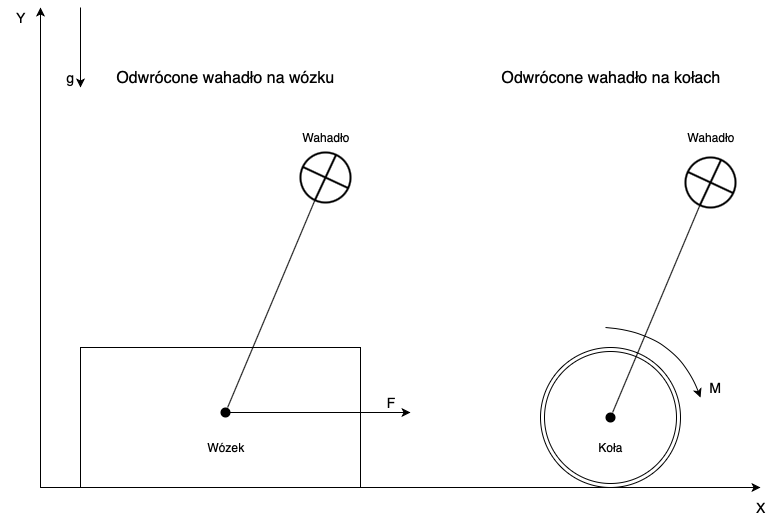
\includegraphics[width=0.75\textwidth]{Rysunki/Rozdzial02/Schemat_wozek_kola.png}
	    \caption{Modele odwróconego wahadła}
	    \label{Modele odwroconego wahadla}
	\end{figure}

\section{Model dynamiki robota balansującego}

W celu ułatwienia implementacji algorytmu sterującego na rzeczywistym robocie, wyprowadzone zostały jego równania dynamiki oraz równania stanu pozwalające na przetestowanie układu sterowania w środowisku \texttt{Matlab Simulink}. W modelu pominięto opory powietrza oraz tarcie pomiędzy wahadłem a kołami oraz kołami a podłożem. Prędkości oraz siły w układzie zostały przedstawione na schemacie \ref{Schemat modelu}

    \begin{figure}[h!]
	    \centering
	    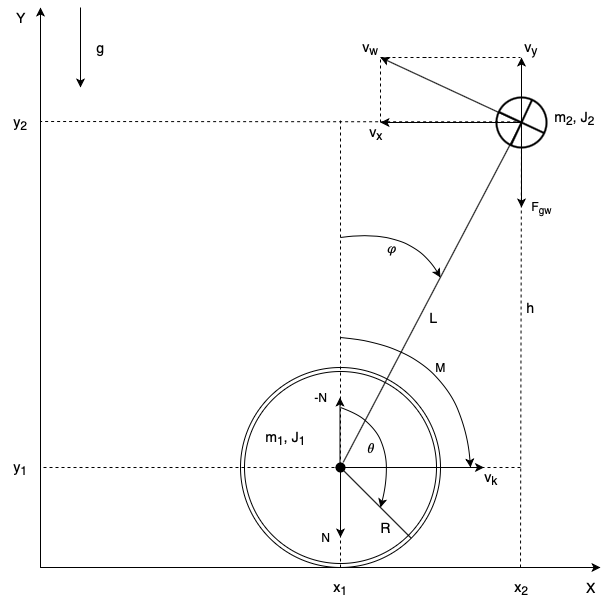
\includegraphics[width=0.75\textwidth]{Rysunki/Rozdzial02/Schemat_modelu_dynamiki.png}
	    \caption{Schemat modelu}
	    \label{Schemat modelu}
	\end{figure}
	
	\newpage
	
Oznaczenia występujące na schemacie modelu dynamiki, przedstawione są w tabeli:
    \begin{table}[h!]
        \centering
        \caption{Oznaczenia wykorzystywane w modelu}
        \label{Oznaczenia}
        \begin{tabular}{|c|l|}
              \hline
              Symbol & Opis\\
              \hline
              $\varphi$ & Kąt wychylenia wahadła od pionu \\
              \hline
              $\theta$ & Kąt obrotu koła względem pionu \\
              \hline
              $x_1, y_1$ & Współrzędne środka połączenia koła z wahadłem \\
              \hline
              $x_2, y_2$ & Współrzędne środka masy wahadła \\
              \hline
              $m_1$ & Masa koła \\
              \hline
              $m_2$ & Masa wahadła \\
              \hline
              $J_1$ & Moment bezwładności koła \\
              \hline
              $J_2$ & Moment bezwładności wahadła \\
              \hline
              $R$ & Promień koła \\
              \hline
              $M$ & Moment siły generowany przez napęd\\
              \hline
              $L$ & Odległość środka masy wahadła od osi obrotu \\
              \hline
              $h$ & Wysokość na jakiej znajduje się środek masy wahadła \\
              \hline
              $g$ & Wektor siły grawitacji \\
              \hline
              $F_{gw}$ & Wektor siły ciężkości oddziałującej na środek masy wahadła \\
              \hline
              $N$ & Wektor siły nacisku koła na podłoże \\
              \hline
              $v_w, v_x, v_x $ & Wektory prędkości środka masy wahadła \\
              \hline
              $v_k$ & Wektor prędkości koła \\
              \hline
        \end{tabular}
    \end{table}
    	
Parametry obiektu eksperymentalnego wykorzystane podczas symulacji i obliczeń:
    \begin{table}[h!]
        \centering
        \caption{Parametry modelu}
        \label{Parametry}
        \begin{tabular}{|c|c|c|}
              \hline
              Symbol & Wartość & Jednostka\\
              \hline
              $m_1$ & $0,02$ & $kg$\\
              \hline
              $m_2$ & $1,2$ & $kg$\\
              \hline
              $R$ & $0,04$ & $m$\\
              \hline
              $L$ & $0,05$ & $m$\\
              \hline
              $J_1$ & $\frac{1}{2}\cdot m_1 \cdot R^2 = 0,000026$ & $kg \cdot m^2$\\
              \hline
              $J_2$ & $\frac{1}{3}\cdot m_2 \cdot L^2 = 0,002$ & $kg \cdot m^2$\\
              \hline
              $g$ & $9,806$ & $\frac{m}{s^2}$\\
              \hline
        \end{tabular}
    \end{table}

Korzystając z funkcji trygonometrycznych i zależności pomiędzy odległością środka masy wahadła od jego początku oraz kątem zakreślonym przez wahadło, można wyznaczyć położenie środka masy wahadła w zależności od położenia środka koła. Dodatkowo wysokość na jakiej znajduje się środek koła, jest jednocześnie jego promieniem $y_2 = R$. Współrzędne środka masy wahadła:
$$
    \left\{
    \begin{array}{lr}
    \frac{x_2-x_1}{L} = sin\varphi \\
    \frac{y_2-y_1}{L} = cos\varphi
    \end{array}
    \right.
    \Rightarrow
    \left\{
    \begin{array}{lr}
    x_2 = x_1 + Lsin\varphi \\
    y_2 = y_1 + Lcos\varphi
    \end{array}
    \right.
    \Rightarrow
    \left\{
    \begin{array}{lr}
    x_2 = x_1 + Lsin\varphi \\
    y_2 = R + Lcos\varphi
    \end{array}
    \right.
$$

Korzystając z twierdzenia odwrotnego do twierdznia Pitagorasa, oraz rachunku różniczkowego (prędkość jako pochodna po czasie z przebytej drogi) można wyznaczyć prędkość środka masy wahadła na podstawie jej składowych w osi x oraz y. Składowe prędkości jako pochodne z przemieszczenia w osi x oraz y
$$
    \left\{
    \begin{array}{c}
    \dot{x}_2 = \dot{x}_1 + Lcos\varphi\dot{\varphi} \\
    \dot{y}_2 = -Lsin\varphi\dot{\varphi}
    \end{array}
    \right.
$$
oraz prędkość wypadkowa wahadła obliczona przy wykorzystaniu twierdzenia odwrotnego do twierdzenia Pitagorasa:
\begin{equation}
    \begin{array}{ll}
    v_w^2 = v_x^2 + v_y^2 \Rightarrow v_w = \sqrt{\dot{x}_2^2 + \dot{y}_2^2} \\ \\
    v_w = \sqrt{\dot{x}_1^2 + 2\dot{x}_1Lcos\varphi\dot{\varphi} + L^2cos^2\varphi\dot{\varphi}^2 + L^2sin^2\varphi\dot{\varphi}^2} = \sqrt{\dot{x}_1^2 + 2\dot{x}_1Lcos\varphi\dot{\varphi} + L^2\dot{\varphi}^2}
    \end{array}
\end{equation}

%---------------------------------------------------------------------------------------------
\subsection{Energia kinetyczna}
Znając prędkość wypadkową wahadła, wyznacza się jego energię kinetyczną, która jest sumą energii kinetycznej ruchu postępowego i energii kinetycznej ruchu obrotowego
$$
    \begin{array}{ll}
    K_w = \frac{1}{2}m_2v_w^2 + \frac{1}{2}J_2\dot{\varphi}^2 = \frac{1}{2}m_2(\dot{x}_1^2 + 2\dot{x}_1Lcos\varphi\dot{\varphi} + L^2\dot{\varphi}^2) + \frac{1}{2}J_2\dot{\varphi}^2
    \end{array}
$$
oraz w analogiczny sposób wyznacza się energię kinetyczną koła
$$
    \begin{array}{ll}
    K_k = \frac{1}{2}m_1\dot{x}_1^2 + \frac{1}{2}J_1\dot{\theta}^2
    \end{array}
$$

Energia kinetyczna układu jest sumą energii kinetycznej wahadła oraz dwóch kół:
\begin{equation}
    \begin{array}{ll}
    K = K_w + 2K_k = \frac{1}{2}m_2(\dot{x}_1^2 + 2\dot{x}_1Lcos\varphi\dot{\varphi} + L^2\dot{\varphi}^2) + \frac{1}{2}J_2\dot{\varphi}^2 + m_1\dot{x}_1^2 + J_1\dot{\theta}^2
    \end{array}
\end{equation}

%---------------------------------------------------------------------------------------------
\subsection{Energia potencjalna}

Środek masy wahadła znajduje się na wysokości $y_2 = m_2g(R + Lcos\varphi)$, a po wstawieniu jej do wzoru na energię potencjalną ciała o masie $m$ znajdującego się na wysokości $h$, otrzymujemy energię potencjalną środka masy wahadła:
$$
    \begin{array}{ll}
    V_w = mgh = m_2gy_2 = m_2g(R + Lcos\varphi)
    \end{array}
$$

Energia potencjalna koła:
$$
    \begin{array}{ll}
    V_k = m_1gR
    \end{array}
$$

Gdyby przyjęto układ współrzędnych, w którym środek koła znajdowałby się na wysokości $y_2 = 0$, to energia potencjalna koła wynosiłaby 0. \\

Energia potencjalna układu jest sumą energii potencjalnej w środku masy wahadła, oraz energii potencjalnej dwóch kół:
\begin{equation}
    \begin{array}{ll}
    V = V_w + 2V_k = m_2g(R + Lcos\varphi) + 2m_1gR
    \end{array}
\end{equation}

%---------------------------------------------------------------------------------------------
\subsection{Równania Eulera--Lagrange'a}

Znając energię kinetyczną oraz potencjalną układu przystąpić można do obliczenia Lagranżjanu \cite{ManipulatoryiRoboty}, który jest różnicą energii kinetycznej oraz potencjalnej układu
\begin{equation}
    \begin{array}{cl}
    \mathcal{L} = K - V \\ \\ 
    \mathcal{L} = \frac{1}{2}m_2(\dot{x}_1^2 + 2\dot{x}_1Lcos\varphi\dot{\varphi} + L^2\dot{\varphi}^2) + m_1\dot{x}_1^2 + J_1\dot{\theta}^2 - m_2g(R + Lcos\varphi) - 2m_1gR
    \label{Lagranżjan}
    \end{array}
\end{equation}
gdzie droga przebyta przez toczące się koło oraz prędkość ruchu postępowego wynosi $x_1 = R\theta$, a co za tym idzie prędkość koła w osi x to $\dot{x}_1 = R\dot{\theta}$, co po wstawieniu do wzoru (\ref{Lagranżjan}) daje ostateczną postać Lagrangianu:
\begin{equation}
    \begin{array}{ll}
    \mathcal{L} = \frac{1}{2}m_2(R^2\dot{\theta}^2 + 2R\dot{\theta}Lcos\varphi\dot{\varphi} + L^2\dot{\varphi}^2) + m_1R^2\dot{\theta}^2 + \\ \\
    + J_1\dot{\theta}^2 - m_2g(R + Lcos\varphi) - 2m_1gR
    \end{array}
\end{equation}

Mając dany Lagranżjan, przystępujemy do wyznaczenie równań Eulera-Lagrange'a drugiego rodzaju, których ogólna postać wygląda następująco
$$
    \begin{array}{ll}
    \frac{d}{dt}\frac{\delta\mathcal{L}}{\delta\dot{q_i}} - \frac{\delta\mathcal{L}}{\delta q_i} = F_i
    \end{array}
$$
gdzie
\begin{itemize}
    \item $\frac{\delta\mathcal{L}}{\delta q_i}$ -- i-ta składowa siły uogólnionej
    \item $\frac{\delta\mathcal{L}}{\delta\dot{q_i}}$ -- i-ta składowa pędu uogólnionego
    \item $F_i$ -- i-ta składowa sił niepotencjalnych
\end{itemize}

W tym przypadku składowe dla zmiennych $\varphi$ oraz $\theta$ wynoszą odpowiednio
$$
    \varphi:
    \left\{
    \begin{array}{ll}
    \frac{\delta\mathcal{L}}{\delta\varphi} = -m_2R\dot{\theta}Lsin\varphi\dot{\varphi}
    \frac{\delta\mathcal{L}}{\delta\dot{\varphi}} = m_2R\dot{\theta}Lcos\varphi + m_2L^2\dot{\varphi} + J_2\dot{\varphi}
    \end{array}
    \right.
$$

$$
    \theta:
    \left\{
    \begin{array}{ll}
    \frac{\delta\mathcal{L}}{\delta\theta} = 0 \\ \\
    \frac{\delta\mathcal{L}}{\delta\dot{\theta}} = m_2R^2\dot{\theta} + m_2RLcos\varphi\dot{\varphi} + 2m_1R^2\dot{\theta} + 2J_1\dot{\theta} 
    \end{array}
    \right.
$$

Mając wszystkie składowe oblicza się jeszcze pochodne po czasie składowych sił uogólnionych i otrzymujemy ostatecznie równania Eulera-Lagrange'a:
\begin{equation}
    \begin{array}{ll}
    \frac{d}{dt}\frac{\delta\mathcal{L}}{\delta\dot{\varphi}} - \frac{\delta\mathcal{L}}{\delta\varphi} = m_2R\Ddot{\theta}Lcos\varphi - m_2R\dot{\theta}sin\varphi\dot{\varphi} + m_2L^2\Ddot{\varphi} + J_2\Ddot{\varphi} + m_2R\dot{\theta}Lsin\varphi\dot{\varphi} + \\ \\
    - m_2gLsin\varphi = m_2R\Ddot{\theta}Lcos\varphi + m_2L^2\Ddot{\varphi} + J_2\Ddot{\varphi} - m_2gLsin\varphi = -M
    \\ \\
    \frac{d}{dt}\frac{\delta\mathcal{L}}{\delta\dot{\theta}} - \frac{\delta\mathcal{L}}{\delta\theta} = m_2R^2\Ddot{\theta} - m_2RLsin\varphi\dot{\varphi}^2 + m_2RLcos\varphi\Ddot{\varphi} + 2m_1R^2\Ddot{\theta} + 2J_1\Ddot{\theta} = M
    \end{array}
\end{equation}
%
gdzie $M$ to moment siły generowany przez napęd. Dla zmiennej $\theta$ ze znakiem dodatnim, ponieważ kierunek obrotu kół jest zgodny z kierunkiem generowanego momentu. Dla zmiennej $\varphi$ z ujemnym znakiem, ponieważ kierunek obrotu wahadła jest przeciwny do działającego momentu siły. 

Równania dynamiki można przedstawić w postaci macierzowej, która jest bardziej czytelna
$$
    \begin{array}{cc}
        \left[ \begin{array}{cc}
        m_2L^2 + J_2 & m_2RLcos\varphi \\
        m_2RLcos\varphi & m_2R^2 + 2m_1R^2 + 2J_1
        \end{array} \right]
        \left[ \begin{array}{c}
        \Ddot{\varphi} \\
        \Ddot{\theta}
        \end{array} \right]
        +
        \left[ \begin{array}{cc}
        0 & 0 \\
        -m_2RLsin\varphi\dot{\varphi} & 0
        \end{array} \right]
        \left[ \begin{array}{c}
        \dot{\varphi} \\
        \dot{\theta}
        \end{array} \right]
        + \\ \\ +
        \left[ \begin{array}{c}
        -m_2gLsin\varphi \\
        0
        \end{array} \right]
        = 
        \left[ \begin{array}{c}
        -M \\
        M
        \end{array} \right]
    \end{array}
$$

Taki model jest jednak nieliniowy i liniowy algorytm sterowania nie zadziałałby dla niego poprawnie, dlatego dokonuje się częściowej linearyzacji modelu w okolicach punktu równowagi, w przypadku w którym chcemy wykorzystać liniowy sterownik. Jednym z punktów równowagi odwróconego wahadła jest jego pionowa pozycja, punkt niestabilny. Drugi punkt równowagi to swobodne zwisanie wahadła, który jest stabilnym punktem równowagi, jednak zostaje on pominięty ze względu na jego brak w rozważanym modelu. Dla punktu równowagi $\varphi \approx 0$ możemy dokonać linearyzacji modelu dla którego
$$
    \left\{
    \begin{array}{c}
    sin\varphi \approx \varphi, \\
    cos\varphi \approx 1, \\
    \dot{\varphi}^2 \approx 0
    \end{array}
    \right.
$$

i zapisać w postaci 
$$
M(q)\Ddot{q} + C(q,\dot{q})\dot{q} + D(q) = u 
$$

gdzie:
\begin{itemize}
    \item $q$ -- wektor uogólnionych współrzędnych,
    \item $\dot{q}$ -- wektor uogólnionych prędkości,
    \item $M(q)$ -- symetryczna, dodatnio określona macierz inercji,
    \item $C(q,\dot{q})$ -- macierz sił Coriolisa i sił dośrodkowych,
    \item $D(q)$ -- wektor oddziaływań potencjalnych,
    \item $u$ -- wektor sterowań.
\end{itemize}

$$
\mathbf{M(q)} =
\left[ \begin{array}{cc}
m_2L^2 + J_2 & m_2RL \\
m_2RL & m_2R^2 + 2m_1R^2 + J_1
\end{array} \right]
$$
\\
$$
\mathbf{C(q,\dot{q})} = \emptyset
$$
\\
$$
\mathbf{D(q)} =
\left[ \begin{array}{c}
-m_2gL \\
0
\end{array} \right]
$$
\\
$$
\mathbf{q} =
\left[ \begin{array}{c}
\varphi \\
\theta \\
\end{array} \right]
,
\mathbf{u} =
\left[ \begin{array}{c}
-M \\
M \\
\end{array} \right]
$$

%---------------------------------------------------------------------------------------------
\subsection{Równania stanu}

W celu łatwiejszego wyznaczenia równań stanu zapisujemy równania dynamiki w następującej formie macierzowej  
$$
E\Ddot{q} + F\dot{q} + Gq = Hu 
$$
w której poszczególne elementy są równe
$$
\mathbf{E} = 
\left[ \begin{array}{cc}
m_2L^2 + J_2 & m_2RL \\
m_2RL & m_2R^2 + 2m_1R^2 + J_1
\end{array} \right]
$$
\\
$$
\mathbf{F} = \emptyset
$$
\\
$$
\mathbf{G} = 
\left[ \begin{array}{cc}
-m_2gL & 0 \\
0 & 0
\end{array} \right]
$$
\\
$$
\mathbf{H} = 
\left[ \begin{array}{c}
-1 \\
1
\end{array} \right]
$$

Mnożąc lewostronnie powyższe równanie przez macierz $\mathbf{E^{-1}}$ i wyznaczając pochodne pierwszego i drugiego rzędu, można przystąpić do sformułowania równań stanu. Przyjmują one postać dwóch równań
\begin{equation}
    \left\{
    \begin{array}{ll}
    \dot{x} = Ax + Bu \\
    y = Cx + Du
    \end{array}
    \right.
\end{equation}
w których:
\begin{itemize}
    \item x -- wektor stanu
    \item y -- wektor wyjścia
    \item u -- wymuszenie
\end{itemize}

$$
\mathbf{x} =
\left[ \begin{array}{c}
\varphi \\
\theta \\
\dot{\varphi} \\
\dot{\theta}
\end{array} \right]
\Rightarrow
\mathbf{\dot{x}} =
\left[ \begin{array}{c}
\dot{\varphi} \\
\dot{\theta} \\
\Ddot{\varphi} \\
\Ddot{\theta}
\end{array} \right]
$$
\\ \\
$$
\mathbf{A} =
\left[ \begin{array}{c|ccc}
\begin{array}{cc}
0 & 0 \\
0 & 0
\end{array}
& 
\begin{array}{cc}
1 & 0 \\
0 & 1
\end{array} \\
\hline
-E^{-1}G & -E^{-1}F
\end{array} \right] 
\quad
\mathbf{B} =
\left[ \begin{array}{c}
0 \\
0 \\
-E^{-1}H
\end{array} \right] 
$$
\\ \\
$$
\mathbf{C} =
\left[ \begin{array}{cccc}
1 & 0 & 0 & 0 \\
0 & 1 & 0 & 0 \\
0 & 0 & 1 & 0 \\
0 & 0 & 0 & 1 \\
\end{array} \right] 
\quad
\mathbf{D} = \emptyset
\quad
\mathbf{u} = M
$$

\newpage

%---------------------------------------------------------------------------------------------
\section{Sterowanie}
Jednym z najprostszych i najpopularniejszych algorytmów sterowania odwróconym wahadłem, jest wykorzystanie układu regulacji ze sprzężeniem zwrotnym oraz regulatora PID. Algorytm zaimplementowano i przetestowano w środowisku \texttt{Matlab Simulink}.

%---------------------------------------------------------------------------------------------
\subsection{Pojedynczy regulator PID}
Zadaniem algorytmu jest utrzymanie wychylenia wahadła w okolicy punktu równowagi, dlatego w takim przypadku jest to układ dosterowany (jedna wielkość regulowana i jedno wymuszenie) i w zupełności wystarczy układ regulacji z pojedynczym regulatorem PID.
\begin{figure}[h!]
    \centering
	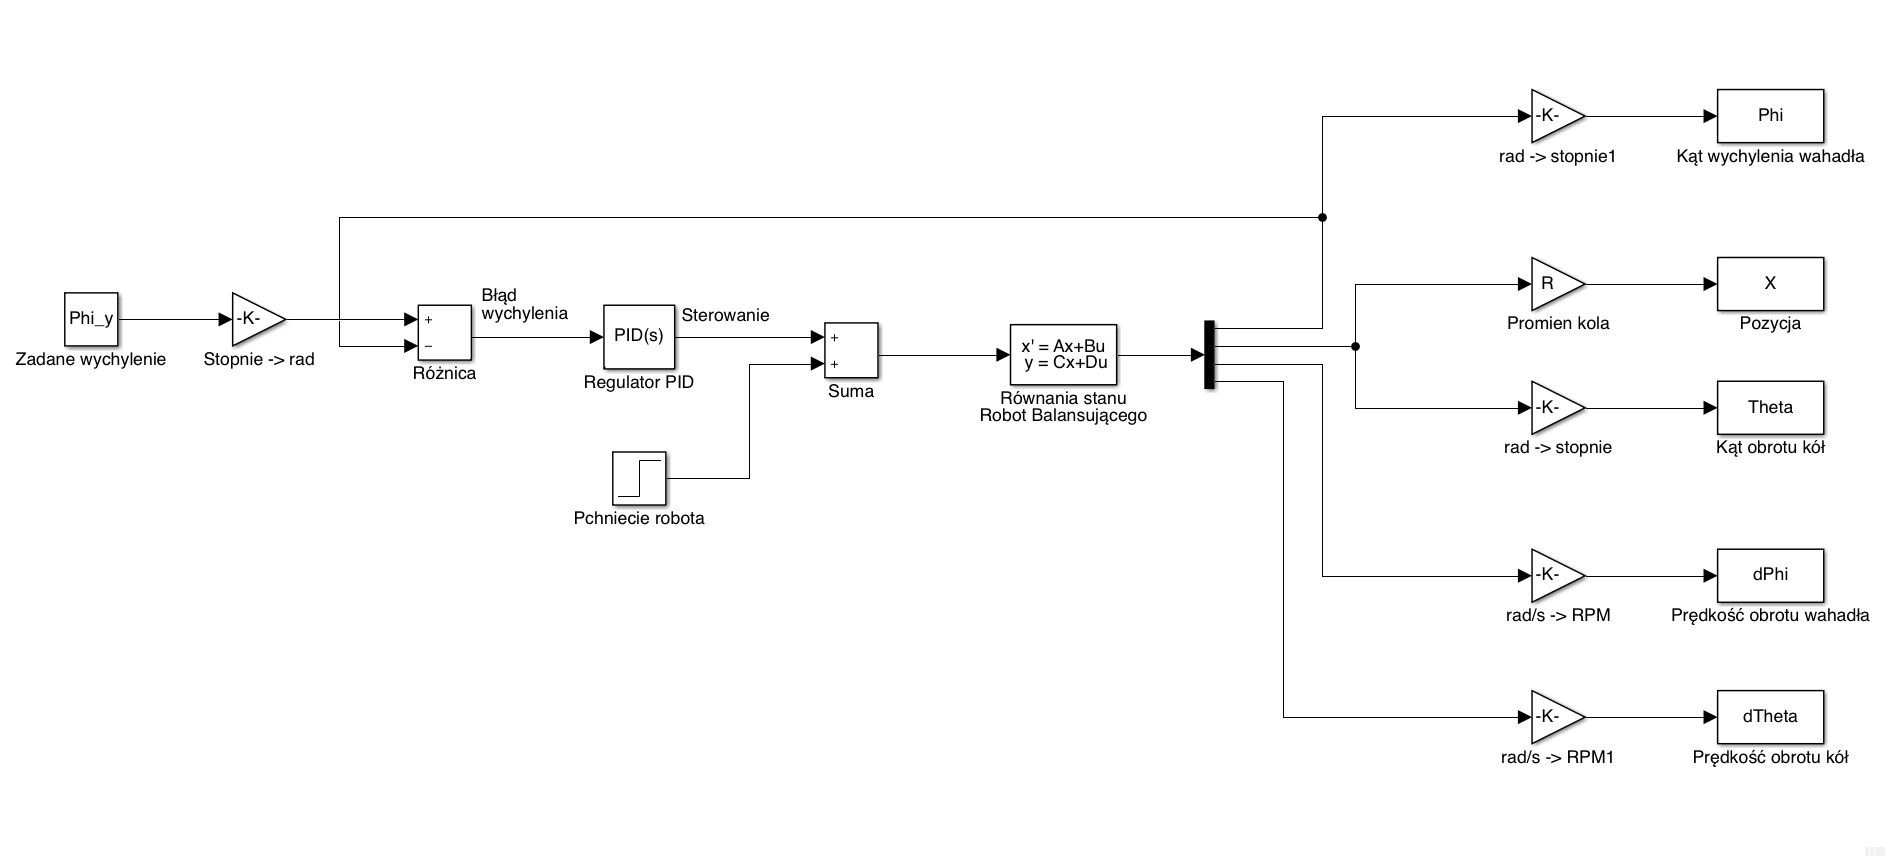
\includegraphics[width=0.9\textwidth]{Rysunki/Rozdzial02/Pojedynczy_PID.png}
	\caption{Schemat sterowania z wykorzystaniem jednego regulatora PID}
\end{figure}

W symulacji bloczki \texttt{gain} służą do przeliczenia radianów na stopnie oraz radiany na sekundę na liczbę obrotów na minutę. Są to jednostki bardziej przystępne i łatwiej sobie wyobrazić z jaką wartością mamy do czynienia.

Parametry regulatora wyznaczone zostały eksperymentalnie i prezentują się następująco
\begin{table}[h!]
    \centering
    \begin{tabular}{|c|c|}
        \hline
        $K_p$ & 10 \\
        \hline
        $K_i$ & 100 \\
        \hline
        $K_d$ & 0.1 \\
        \hline
        Wejście & Zadana prędkość kół \\
        \hline
        Wyjście & Zadany kąt wychylenia \\
        \hline
    \end{tabular}
        
    \caption{Parametry regulatora PID}
    \label{Parametry PID}
\end{table}

\begin{figure}
    Wizualizację tego jak zachowuje się wahadło podczas implementacji algorytmu i strojenia regulatora, daje prosta animacja pozycji kół oraz wychylenia wahadła. Na obrazku widzimy, że pomimo utrzymanego wychylenia wahadła w zadanej pozycji, położenie obiektu dryfuje w nieskończoność przy nieskończonym czasie symulacji.
    \\ 
    \begin{center}
        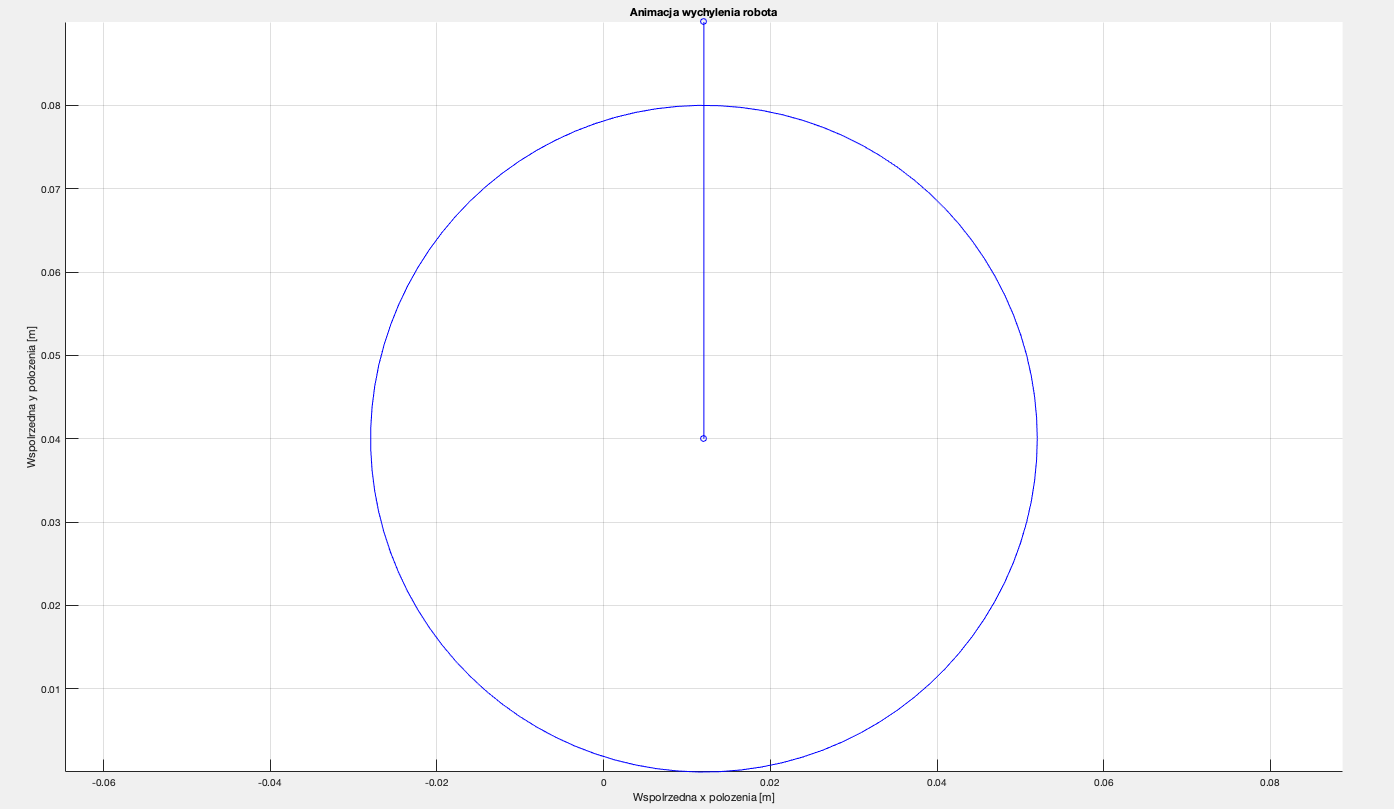
\includegraphics[width=0.9\textwidth]{Rysunki/Rozdzial02/Pojedynczy_PID_animacja.png}
	    \caption{Pozycja wahadła po 2 sekundach symulacji w płaszczyźnie XY}
    \end{center}
	\label{PID animacja}
\end{figure}

\begin{figure}
    Na początku symulacji wahadło znajduje się w punkcie równowagi, po czym w 1 sekundzie następuje skok jednostkowy, który symuluje pchnięcie robota generujące moment obrotowy o wartości 1 Nm. Takie wymuszenie wychyla wahadło w szczytowym momencie do wartości około 1.6 stopnia, oraz zmusza napęd do wygenerowania prędkości obrotowej kół na poziomie około 20 RPM. Jak widać na wykresie, czas stabilizacji wynosi około 0.4 s, przy czym pozycja robota zbiega do nieskończoności.
    \\
    \begin{center}
        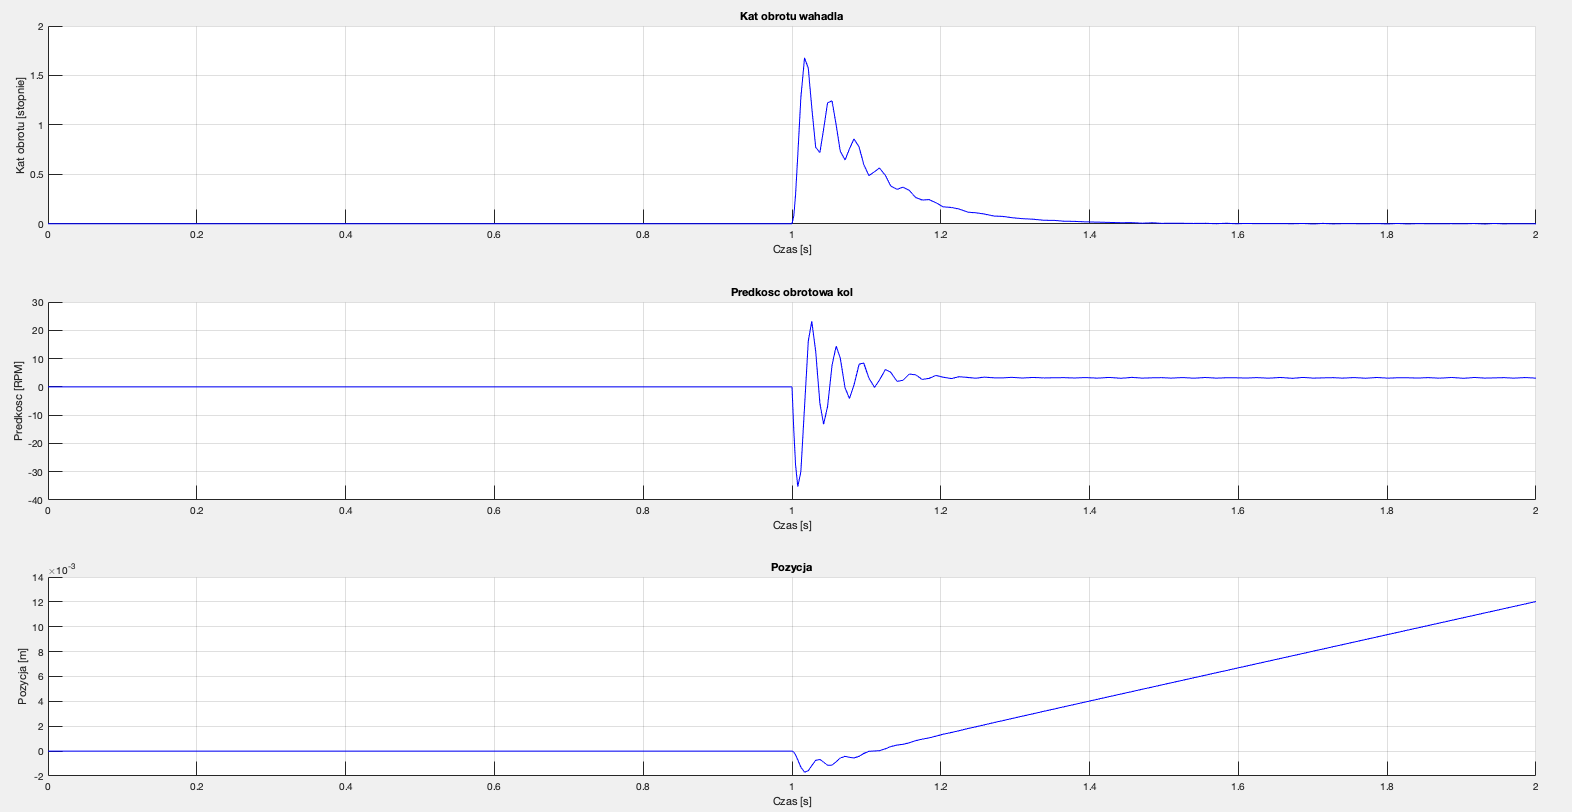
\includegraphics[width=0.9\textwidth]{Rysunki/Rozdzial02/Pojedynczy_PID_wykresy.png}
	    \caption{Wykres dla układu z jednym regulatorem: nr.1 -- wychylenie wahadła, nr.2 -- prędkość obrotu kół, nr.3 -- pozycja kół}
    \end{center}
	\label{Wykresy PID1}
\end{figure}

\newpage

\subsection{Podwójny regulator PID}
W przypadku, w którym zadaniem algorytmu jest nie tylko utrzymanie wychylenia wahadła, ale również utrzymanie zadanej pozycji czy prędkości kół, to pojawia się problem, ponieważ układ jest niedosterowany (dwie wielkości regulowane i jedno wymuszenie), który rozwiązuje zastosowanie dwóch regulatorów PID połączonych kaskadowo. Pierwszy regulator odpowiedzialny jest za utrzymanie zadanej prędkości kół lub pozycji, a drugi za utrzymanie prawidłowego kąta wychylenia wahadła. 

\begin{figure}[h!]
    \centering
	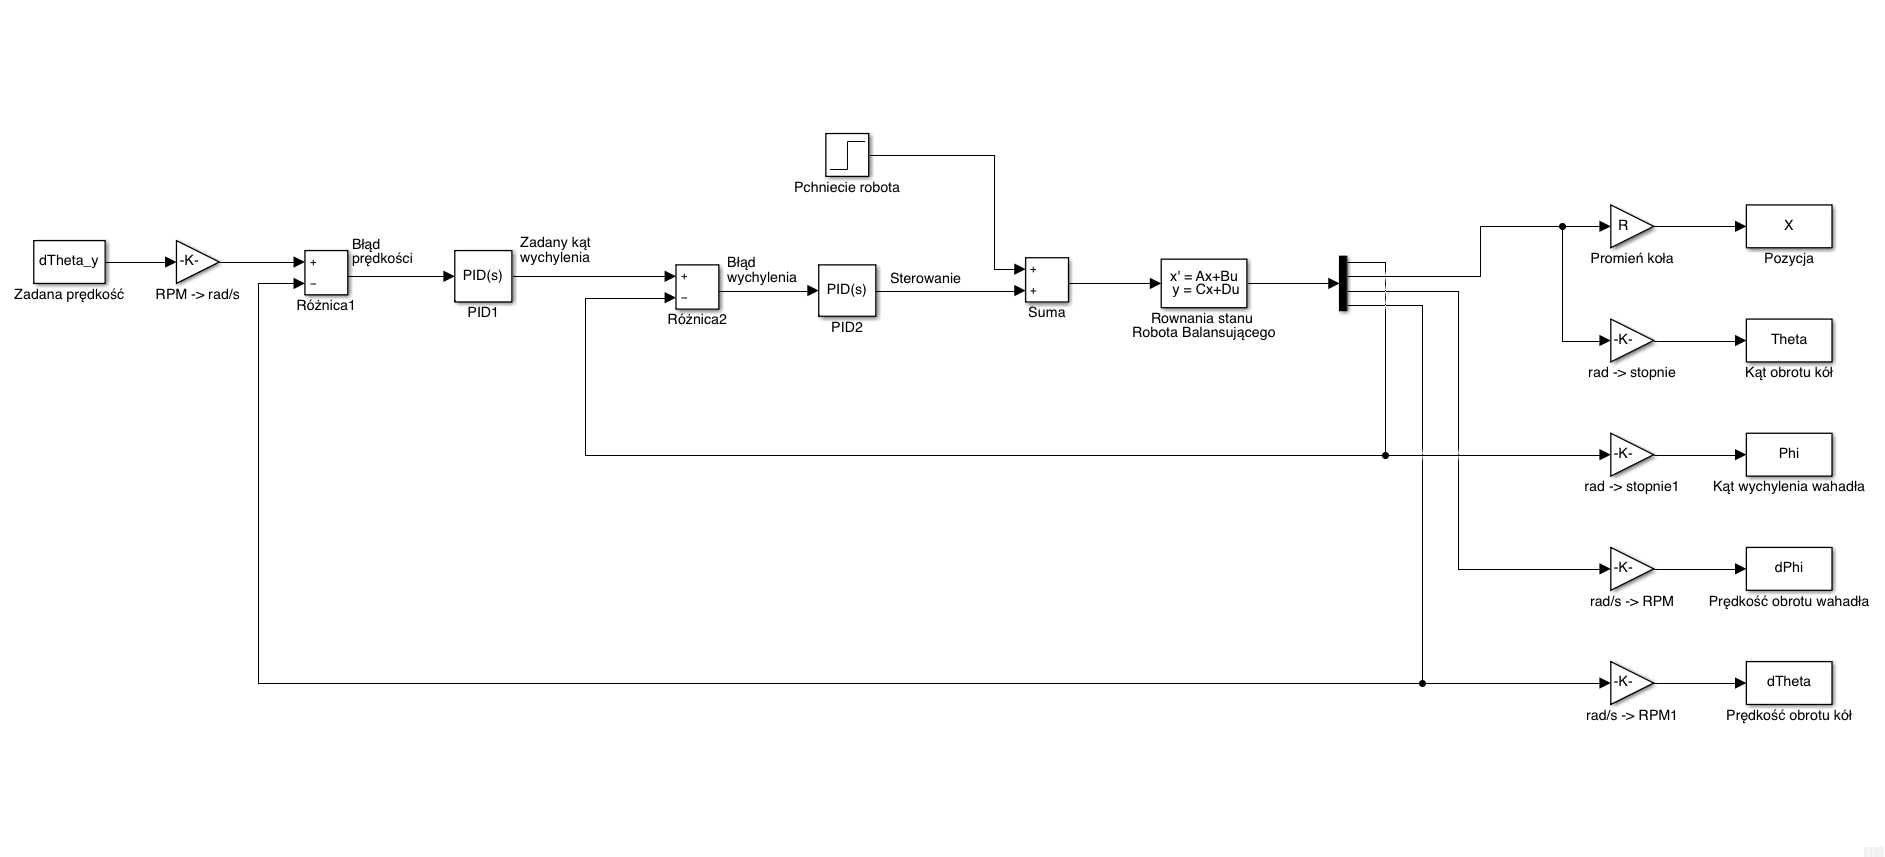
\includegraphics[width=0.9\textwidth]{Rysunki/Rozdzial02/Podwojny_PID.png}
	\caption{Schemat sterowania z wykorzystaniem dwóch regulatorów PID połączonych kaskadowo}
\end{figure}

Dla kaskadowego połączenia regulatorów, nastawy również zostały dobrane eksperymentalnie. Nastawy regulatora odpowiedzialnego za utrzymanie kąta wychylenia wahadła pozostały identyczne, jak w przypadku układu z pojedynczym regulatorem.
\begin{table}[h!]
    \centering
    \begin{tabular}{|c|c|}
        \hline
        $K_p$ & 20 \\
        \hline
        $K_i$ & 25 \\
        \hline
        $K_d$ & 0.02 \\
        \hline
        Wejście & Zadana prędkość kół \\
        \hline
        Wyjście & Zadany kąt wychylenia \\
        \hline
    \end{tabular}
        
    \caption{Parametry regulatora PID1}
    \label{Parametry PID1}
\end{table}

\begin{table}[h!]
    \centering
    \begin{tabular}{|c|c|}
        \hline
        $K_p$ & 10 \\
        \hline
        $K_i$ & 100 \\
        \hline
        $K_d$ & 0.1 \\
        \hline
        Wejście & Zadany kąt wychylenia \\
        \hline
        Wyjście & Sterowanie \\
        \hline
    \end{tabular}
        
    \caption{Parametry regulatora PID2}
    \label{Parametry PID2}
\end{table}

\begin{figure}[h!]
    Zadana prędkość kątowa kół równa zeru, sprawia że wahadło utrzymuje się w punkcie równowagi oraz wyeliminowano efekt dryfowania pozycji.
    \\ \\
    \begin{center}
        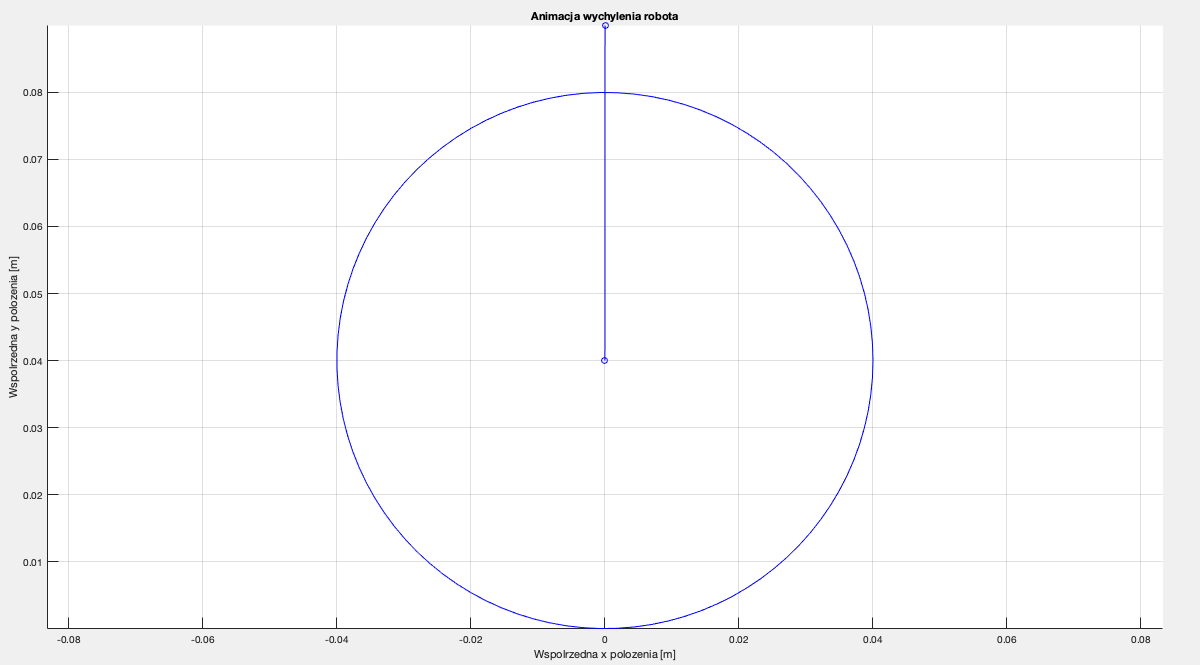
\includegraphics[width=0.9\textwidth]{Rysunki/Rozdzial02/Podwojny_PID_animacja.png}
	    \caption{Pozycja wahadła po 5 sekundach symulacji w płaszczyźnie XY}
    \end{center}
\end{figure}

\begin{figure}[h!]
    Jednym z efektów ubocznych zastosowania bardziej skomplikowanego układu regulacji jest wydłużenie samego czasu stabilizacji kąta wychylenia wahadła, co jest widoczne na wykresie.
    \\ \\ 
    \begin{center}
        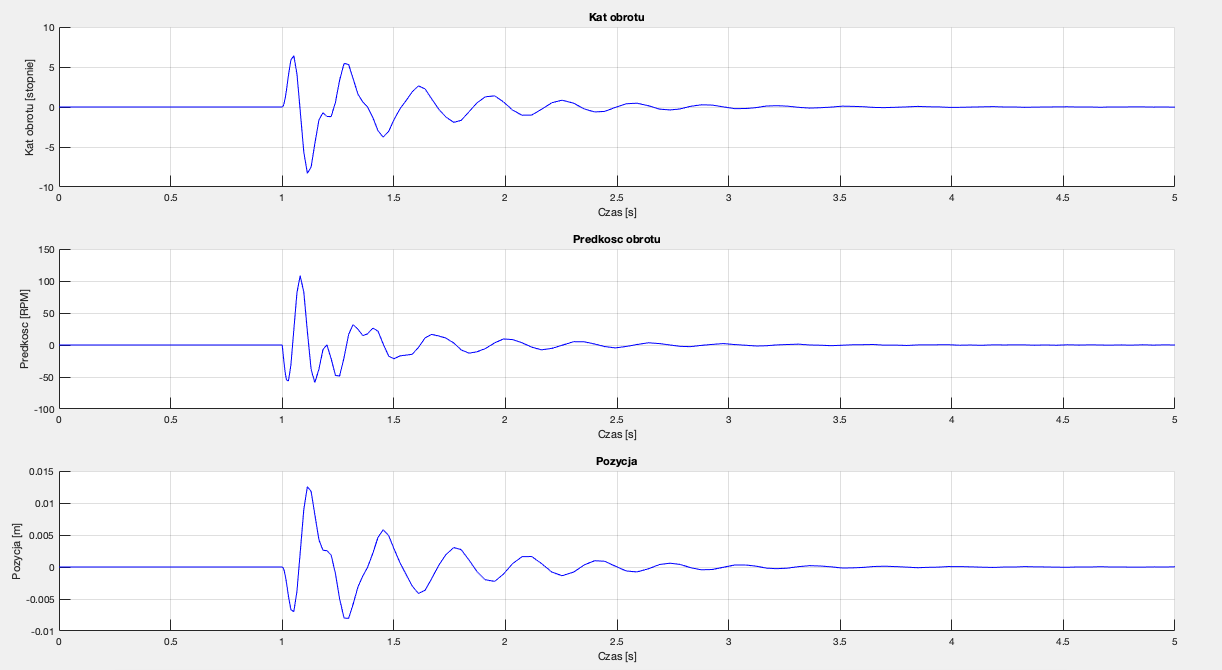
\includegraphics[width=0.9\textwidth]{Rysunki/Rozdzial02/Podwojny_PID_wykresy.png}
	    \caption{Wykres dla układu z dwoma regulatorami: nr.1 -- wychylenie wahadła, nr.2 -- prędkość obrotu kół, nr.3 -- pozycja kół}
    \end{center}
	\label{Wykresy PID2}
\end{figure}
\chapter{Akwizycja i wykorzystanie danych z czujników ruchu}

Wprowadzone oznaczenia, w celu zwiększenia czytelności macierzy rotacji
$$
    \begin{array}{ccc}
        s_{\varphi} = sin\varphi, & s_{\theta} = sin\theta, & s_{\psi} = sin\psi \\
        c_{\varphi} = cos\varphi, & c_{\theta} = cos\theta, & c_{\psi} = cos\psi
    \end{array}
$$

Macierze rotacji
$$
    \mathbf{R_x(\varphi)} =
    \left[
        \begin{array}{ccc}
            1 & 0 & 0 \\
            0 & c_{\varphi} & s_{\varphi} \\
            0 & -s_{\varphi} & c_{\varphi}
        \end{array}
    \right]
    %
    \mathbf{R_y(\theta)} =
    \left[
        \begin{array}{ccc}
            c_{\theta} & 0 & -s_{\theta} \\
            0 & 1 & 0 \\
            s_{\theta} & 0 & c_{\theta}
        \end{array}
    \right]
    %
    \mathbf{R_z(\psi)} =
    \left[
        \begin{array}{ccc}
            c_{\psi} & s_{\psi} & 0 \\
            -s_{\psi} & c_{\psi} & 0 \\
            0 & 0 & 1
        \end{array}
    \right]
$$
%
$$
    \mathbf{R} =
    \mathbf{R_x(\varphi)R_y(\theta)R_z(\psi)} =
    \left[
        \begin{array}{ccc}
            c_{\theta}c_{\psi} & c_{\theta}s_{\psi} & s_{\theta} \\
            c_{\psi}s_{\theta}s_{\varphi} - s_{\varphi}s_{\psi} & c_{\varphi}c_{\psi} + s_{\theta}s_{\varphi}s_{\psi} & c_{\theta}s_{\varphi} \\
            c_{\varphi}c_{\psi}s_{\theta} + s_{\varphi}s_{\psi} & c_{\varphi}s_{\theta}s_{\psi} - c_{\psi}s_{\varphi} & c_{\theta}c_{\varphi}
        \end{array}
    \right]
$$
%----------------------------------------------------------------------------------------------------------------
\section{Żyroskop}

\begin{figure}[!htb]
    \centering
    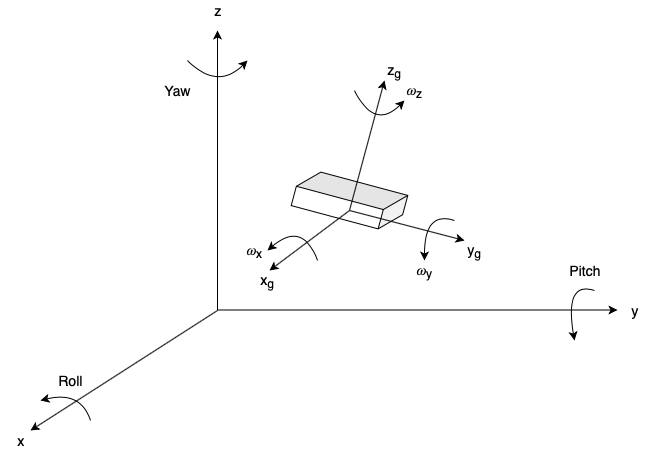
\includegraphics[width=0.6\textwidth]{Rysunki/Rozdzial03/Zyroskop.png}
    \caption{Wizualizacja odczytów żyroskopu}
\end{figure}

Wektor prędkości kątowych
$$
    \mathbf{\omega} = 
    \left[
    \begin{array}{c}
        \omega_x \\
        \omega_y \\
        \omega_z
    \end{array}
    \right]
$$

W przypadku, w którym interesuje nas jednowymiarowe określenie orientacji, możemy go wyznaczyć poprzez scałkowanie prędkości kątowej w danej osi \cite{Akwizycja}
$$
    \alpha_t = \int_{0}^{t} \omega \Delta t = \alpha_{t-1} + \omega_t \Delta t
$$

Problem pojawia się w momencie, w którym chcemy znać orientację czujnika w przestrzeni trójwymiarowej. Żyroskop mierzy prędkości kątowe w osiach swojego lokalnego układu współrzędnych i jeśli dokona się zmiany orientacji czujnika względem układu, w którym wyznaczamy orientację, to wyniki będą niepoprawne. W takim przypadku, należy skorzystać ze wzoru na prędkość kątową w przestrzeni, korzystając z własności $R^T=R^{-1}$, która wynika z tego, że macierz R jest ortogonalna.
\begin{equation}
    \left[\omega\right] = \dot{R}R^T \Rightarrow \dot{R} = R \left[\omega\right]
    \label{Predkosc obrotowa}
\end{equation}
gdzie
$$
    \mathbf{\left[\omega\right]} = 
    \left[
    \begin{array}{ccc}
        0 & -\omega_z & \omega_y \\
        \omega_z & 0 & -\omega_x \\
        -\omega_y & \omega_x & 0
    \end{array}
    \right]
$$
Elementami równania (\ref{Predkosc obrotowa}), które chcemy wyznaczyć są elementy macierzy \textbf{R}. Dokonuje się tego poprzez zapisanie równania w postaci równania różniczkowego
$$
\dot{R} = R\left[\omega\right]
$$
którego rozwiązaniem jest
$$
    R_t \approx R_{t-1}(I_{3x3}+\left[\omega\right] \Delta t)
$$

$$
    \left[
    \begin{array}{ccc}
        r_{11} & r_{12} & r_{13} \\
        r_{21} & r_{22} & r_{23} \\
        r_{31} & r_{32} & r_{33} \\
    \end{array}
    \right]_t
    =
    \left[
    \begin{array}{ccc}
        r_{11} & r_{12} & r_{13} \\
        r_{21} & r_{22} & r_{23} \\
        r_{31} & r_{32} & r_{33} \\
    \end{array}
    \right]_{t-1}
    %
    \left[
    \begin{array}{ccc}
        1 & -\omega_z\Delta t & \omega_y\Delta t \\
        \omega_z\Delta t & 1 & -\omega_x\Delta t \\
        -\omega_y\Delta t & \omega_x\Delta t & 1 \\
    \end{array}
    \right]
$$
gdzie macierz \textbf{R} w chwili $t=0$ dla zerowych wartości kątów, wynosi
$$
    \mathbf{R_{0}} =
    \left[
    \begin{array}{ccc}
        1 & 0 & 0 \\
        0 & 1 & 0 \\
        0 & 0 & 1
    \end{array}
    \right]
$$

Mając rozwiązanie równania różniczkowego, możemy obliczyć elementy macierzy $R_t$ oraz kąty Eulera na podstawie odpowiednich elementów tej macierzy
\begin{equation}
    \begin{array}{c}
        Roll(\varphi) = arctan(\frac{r_{32}}{r_{33}}) \\ \\
        Pitch(\theta) = arcsin(-r_{31}) \\ \\
        Yaw(\psi) = arctan(\frac{r_{21}}{r_{11}})
    \end{array}
\end{equation}

%----------------------------------------------------------------------------------------------------------------
\clearpage
\section{Akcelerometr}

\begin{figure}[!htb]
    \centering
    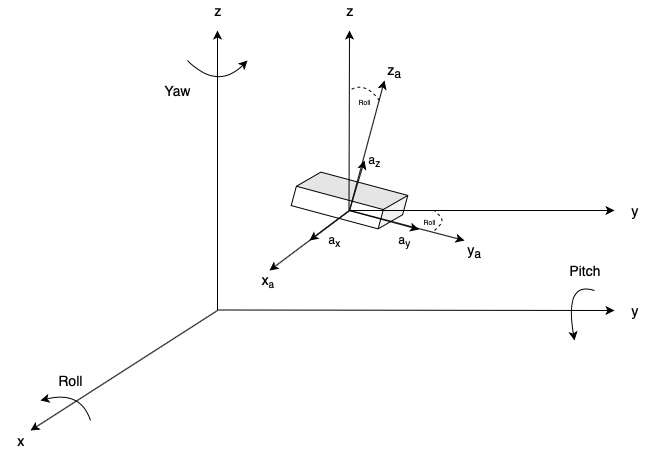
\includegraphics[width=0.6\textwidth]{Rysunki/Rozdzial03/Akcelerometr.png}
    \caption{Wizualizacja odczytów akcelerometru}
\end{figure}

Wektor przyspieszeń w osiach akcelerometru
$$
    \mathbf{a} = 
    \left[
    \begin{array}{cc}
        a_x \\
        a_y \\
        a_z
    \end{array}
    \right]
$$

Znormalizowany wektor równoległy do osi Z
$$
    \mathbf{(g_z)} =
    \left[
        \begin{array}{c}
            0 \\
            0 \\
            1
        \end{array}
    \right]
$$

Orientacja w przestrzeni RPY znormalizowanego wektora grawitacji
$$
R g_z = 
\left[
    \begin{array}{ccc}
        c_{\theta}c_{\psi} & c_{\theta}s_{\psi} & s_{\theta} \\
        c_{\psi}s_{\theta}s_{\varphi} - s_{\varphi}s_{\psi} & c_{\varphi}c_{\psi} + s_{\theta}s_{\varphi}s_{\psi} & c_{\theta}s_{\varphi} \\
        c_{\varphi}c_{\psi}s_{\theta} + s_{\varphi}s_{\psi} & c_{\varphi}s_{\theta}s_{\psi} - c_{\psi}s_{\varphi} & c_{\theta}c_{\varpi}
    \end{array}
\right]
\left[
    \begin{array}{c}
        0 \\
        0 \\
        1
    \end{array}
\right]
= 
\left[
    \begin{array}{c}
        -s_{\theta} \\
        c_{\theta}s_{\varphi} \\
        c_{\theta}c_{\varphi}
    \end{array}
\right]
$$

Orientację akcelerometru mierzy się względem wektora grawitacji, dzięki czemu można zapisać, że
\begin{equation}
    \mathbf{a} =
    \left[
        \begin{array}{c}
            -s_{\theta} \\
            c_{\theta}s_{\varphi} \\
            c_{\theta}c_{\varphi}
        \end{array}
    \right]
    \Rightarrow
    n
    \left[
        \begin{array}{c}
            a_x \\
            a_y \\
            a_z
        \end{array}
    \right]
    =
    \left[
        \begin{array}{c}
            -s_{\theta} \\
            c_{\theta}s_{\varphi} \\
            c_{\theta}c_{\varphi}
        \end{array}
    \right]
    \label{Orientacja akcelerometru}
\end{equation}
\\
gdzie
\begin{itemize}
    \item $a_x$ -- odczyt akcelerometru w osi x
    \item $a_y$ -- odczyt akcelerometru w osi y
    \item $a_z$ -- odczyt akcelerometru w osi z
    \item $n = \frac{1}{\sqrt{a_x^2 + a_y^2 + a_z^2}}$ 
\end{itemize}

Korzystając ze wzoru (\ref{Orientacja akcelerometru}) zapisujemy go w postaci układu równań
$$
    \left\{
        \begin{array}{l}
            na_x = -sin\theta\\
            na_y = cos\theta sin\varphi\\
            na_z = cos\theta cos\varphi
        \end{array}
    \right.
    \Rightarrow
    \left\{
        \begin{array}{l}
            sin\theta = -na_x \\
            cos\theta = n\sqrt{a_y^2 + a_z^2} \\
            sin\varphi = \frac{na_y}{cos\theta} \\
            cos\varphi = \frac{na_z}{cos\theta}
        \end{array}
    \right.
$$
i wyliczamy zależności trygonometryczne, z których otrzymujemy rotacje akcelerometru względem osi x oraz y
\begin{equation}
    \begin{array}{l}
        tg\varphi = \frac{sin\varphi}{cos\varphi} = \frac{a_y}{a_z} \Rightarrow Roll(\varphi) = arctg(\frac{a_y}{a_z}) \\ \\
        tg\theta = \frac{sin\theta}{cos\theta} = \frac{-a_x}{\sqrt{a_y^2+a_z^2}} \Rightarrow Pitch(\theta) = arctg\left(\frac{-a_x}{\sqrt{a_y^2+a_z^2}}\right)
    \end{array}
\end{equation}

Niestety, ale z racji tego, że orientację akcelerometru wyliczamy względem wektora grawitacji nie ma możliwości obliczenia rotacji względem osi Z, czyli kąta Yaw($\psi$).

%----------------------------------------------------------------------------------------------------------------
\section{Magnetometr}

\begin{figure}[h!]
    \centering
    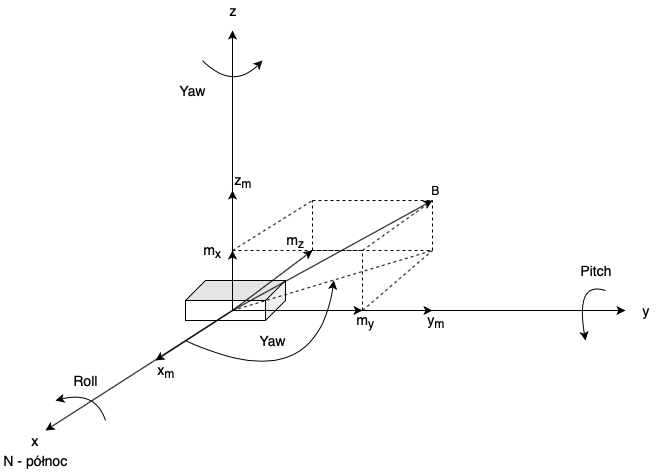
\includegraphics[width=0.6\textwidth]{Rysunki/Rozdzial03/Magnetometr.png}
    \caption{Wizualizacja odczytów magnetometru}
    \label{Rotacja magnetometru}
\end{figure}

\begin{figure}[h!]
    \centering
    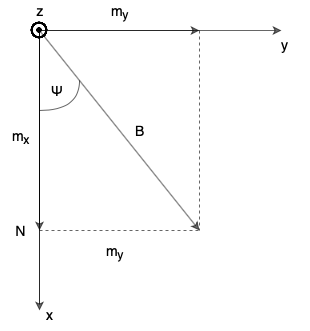
\includegraphics[width=0.3\textwidth]{Rysunki/Rozdzial03/Magnetometr_odchylenie.png}
    \caption{Odchylenie magnetometru od wektora północy magnetycznej}
    \label{Rotacja magnetometru}
\end{figure}

Wektor pola magnetycznego (odczyty magnetometru)
$$
    \mathbf{B} = 
    \left[
    \begin{array}{c}
        m_x \\
        m_y \\
        m_z
    \end{array}
    \right]
$$

Rotacja magnetometru wokół osi Z (odchylenie od wektora pola magnetycznego), przy założeniu, że wartości kątów Roll i Pitch są zerowe (brak odchylenia magnetometru od płaszczyzny XY)
\begin{equation}
    tg\psi = \frac{sin\psi}{cos\psi} = \frac{m_y}{m_x} \Rightarrow Yaw(\delta) = arctg\left(\frac{m_y}{m_x}\right)
    \label{Odchylenie magnetometru}
\end{equation}

Niestety w przypadku, w którym odchylimy magnetometr względem osi x lub y, obliczona według wzoru (\ref{Odchylenie magnetometru}) wartość obrotu wokół osi Z będzie nieprawidłowa, ponieważ zmieni się odczyt magnetometru w osiach x i y oraz z. W celu zniwelowania tego efektu dokonuje się kompensacji kąta wychylenia magnetometru.

%----------------------------------------------------------------------------------------------------------------
\subsection{Kompensacja kąta wychylenia}
Kompensacja kąta wychylenia magnetometru, to nic innego jak uwzględnienie w obliczeniach rotacji wokół osi x i y, wyznaczonych, np. za pomocą akcelerometru.

Wektor pola magnetycznego po kompensacji kąta wychylenia
\begin{equation}
    \begin{array}{c}
        \mathbf{B^{k}} = R_x(\varphi)R_y(\theta)B 
        \\ \\
        \left[
            \begin{array}{c}
                b^k_x \\
                b^k_y \\
                b^k_z
            \end{array}
        \right]
        =
        \left[
            \begin{array}{ccc}
                c_{\theta} & 0 & -s_{\theta} \\
                s_{\varphi}s_{\theta} & c_{\varphi} & s_{\varphi}c_{\theta} \\
                c_{\varphi}s_{\theta} & -s_{\varphi} & c_{\varphi}c_{\theta}
            \end{array}
        \right]
        \left[
            \begin{array}{c}
                m_x \\
                m_y \\
                m_z
            \end{array}
        \right]
        =
        \left[
            \begin{array}{c}
                c_{\theta}m_x - s_{\theta}m_z \\
                s_{\varphi}s_{\theta}m_x + c_{\varphi}m_y + s_{\varphi}c_{\theta}m_z \\
                c_{\varphi}s_{\theta}m_x - s_{\varphi}m_y + c_{\varphi}c_{\theta}m_z
            \end{array}
        \right]
    \end{array}
\end{equation}

Rotacja magnetometru wokół osi Z (odchylenie od wektora pola magnetycznego), po kompensacji kąta wychylenia magnetometru
\begin{equation}
    Yaw(\psi) = arctg\left(\frac{b^k_y}{b^k_x}\right) = arctg\left(\frac{s_{\varphi}s_{\theta}m_x + c_{\varphi}m_y + s_{\varphi}c_{\theta}m_z}{c_{\theta}m_x - s_{\theta}m_z}\right)
    \label{Odchylenie po kompensacji}
\end{equation}

%----------------------------------------------------------------------------------------------------------------
\subsection{Deklinacja magnetyczna}
W celu uzyskania dokładniejszego pomiaru uzależnionego od aktualnej pozycji na Ziemi uwzględnia się deklinację magnetyczną, która dla Wrocławia wynosi
$$
    \delta = 4^{o}E8'E \approx 4,13^{o}E
$$
co daje ostateczną postać wzoru na wskazanie magnetometru, przy założeniu, że kąt Yaw obliczony jest w stopniach, a nie w radianach
$$
   Yaw(\psi) = Yaw(\psi) + \delta = Yaw(\psi) + 4,13^o 
$$

%----------------------------------------------------------------------------------------------------------------
\subsection{Kompensacja efektu ,,Hard Iron'' oraz ,,Soft Iron''}

Nieskalibrowane odczyty magnetometru zostały przedstawione na rysunku \ref{Magnetometr nieskalibrowany}. Na wykresach widoczne są elipsy przesunięte względem punktu (0,0) na wykresie. Odczyty dla skalibrowanego magnetometru na płaszczyznach XY, XZ oraz YZ powinny mieć swój środek w punkcie (0,0), czyli kulą o środku w punkcie (0,0,0) w przestrzeni XYZ.

\begin{figure}[h!]
    \centering
    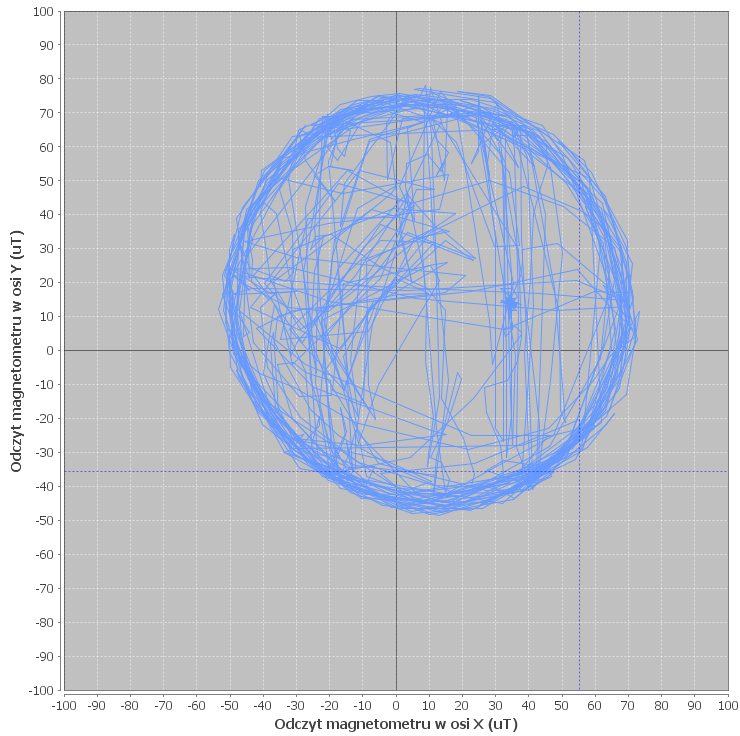
\includegraphics[width=0.5\textwidth]{Rysunki/Rozdzial03/Magnetometr_nieskalibrowany_XY.png}
    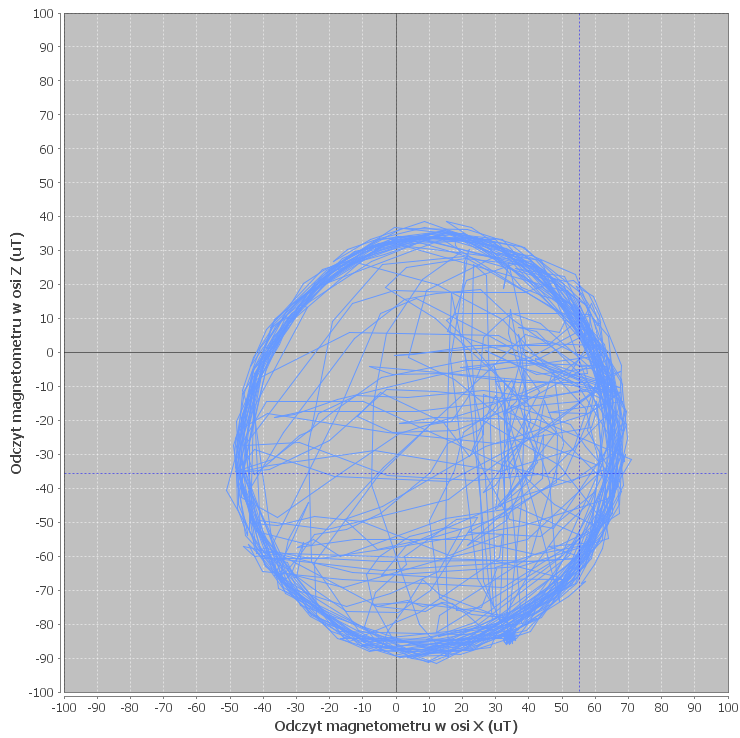
\includegraphics[width=0.5\textwidth]{Rysunki/Rozdzial03/Magnetometr_nieskalibrowany_XZ.png}
    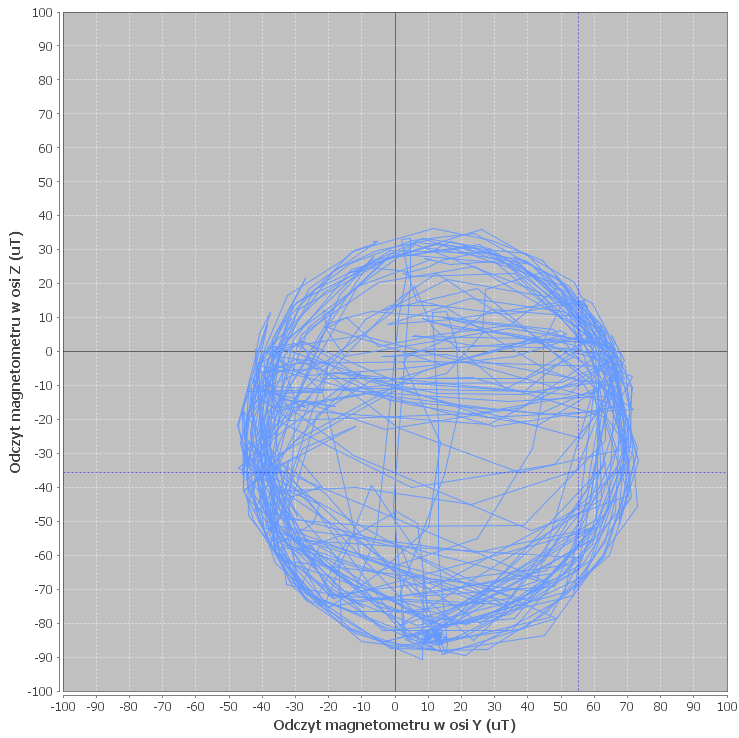
\includegraphics[width=0.5\textwidth]{Rysunki/Rozdzial03/Magnetometr_nieskalibrowany_YZ.png}
    \caption{Odczyty dla nieskalibrowanego magnetometru}
    \label{Magnetometr nieskalibrowany}
\end{figure}

Efekt ,,Hard Iron'' (wpływ ferromagnetyków twardych) kompensuje się poprzez przesunięcie odczytów na środek układu współrzędnych o wyznaczony offset. Przesunięcie wyznacza się na podstawie maksymalnej oraz minimalnej wartości odczytu w danej osi, według następujących wzorów
$$
    \begin{array}{c}
        offset(m_x) = \frac{max(m_x) + min(m_x)}{2} \\ \\
        offset(m_y) = \frac{max(m_y) + min(m_y)}{2} \\ \\
        offset(m_z) = \frac{max(m_z) + min(m_z)}{2}
    \end{array}
$$

Efekt ,,Soft Iron'' (wpływ ferromagnetyków miękkich), który objawia się zniekształceniem odczytów, które powinny tworzyć idealny okrąg na płaszczyźnie, należy skompensować przeskalowując odczyty o wartości wyliczane według następujących wzorów
$$
    \begin{array}{c}
        a(m_x) = \frac{max(m_x) - min(m_x)}{2}, a(m_y) = \frac{max(m_y) - min(m_y)}{2}, a(m_z) = \frac{max(m_z) - min(m_z)}{2} \\ \\
        b = \frac{a(m_x) + a(m_y) + a(m_z)}{3} \\ \\
        scale(m_x) = \frac{b}{a(m_x)}, scale(m_y) = \frac{b}{a(m_y)}, scale(m_z) = \frac{b}{a(m_z)} 
    \end{array}
$$

Na rysunku \ref{Magnetometr skalibrowany} widać, że odczyty dla magnetometru zostały skalibrowane. Przesunięcia odczytów we wszystkich osiach oraz delikatne zniekształcenie dla odczytu XZ zostały skompensowane. Ostateczną postać wektora odczytów magnetometru oblicza się według wzoru (\ref{Ostateczny wektor magnetometr})
\begin{equation}
    \begin{array}{c}
        \left[
            \begin{array}{c}
                m_x \\
                m_y \\
                m_z
            \end{array}
        \right]
        =
        \left[
            \begin{array}{c}
                m_x - offset(m_x) \\
                m_y - offset(m_y) \\
                m_z - offset(m_z)
            \end{array}
        \right]
        \left[
            \begin{array}{c}
                scale(m_x) \\
                scale(m_y) \\
                scale(m_z)
            \end{array}
        \right]
    \end{array}
    \label{Ostateczny wektor magnetometr}
\end{equation}

\begin{figure}[h!]
    \centering
    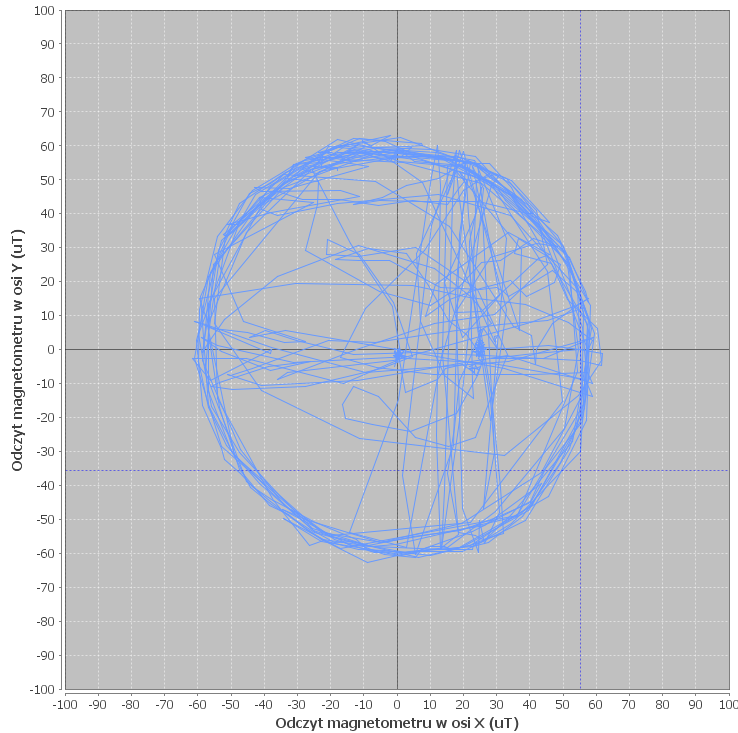
\includegraphics[width=0.5\textwidth]{Rysunki/Rozdzial03/Magnetometr_skalibrowany_hardiron_XY.png}
    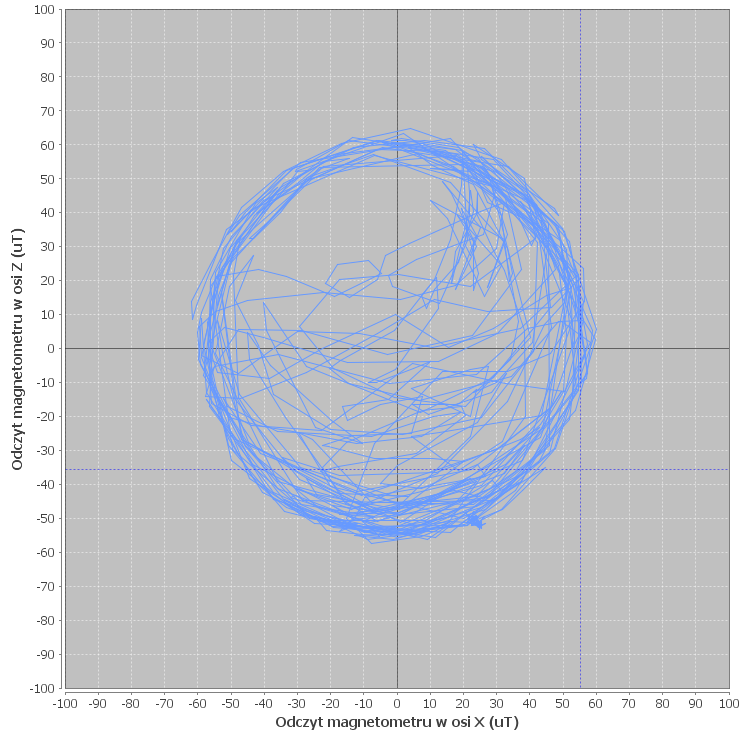
\includegraphics[width=0.5\textwidth]{Rysunki/Rozdzial03/Magnetometr_skalibrowany_hardiron_XZ.png}
    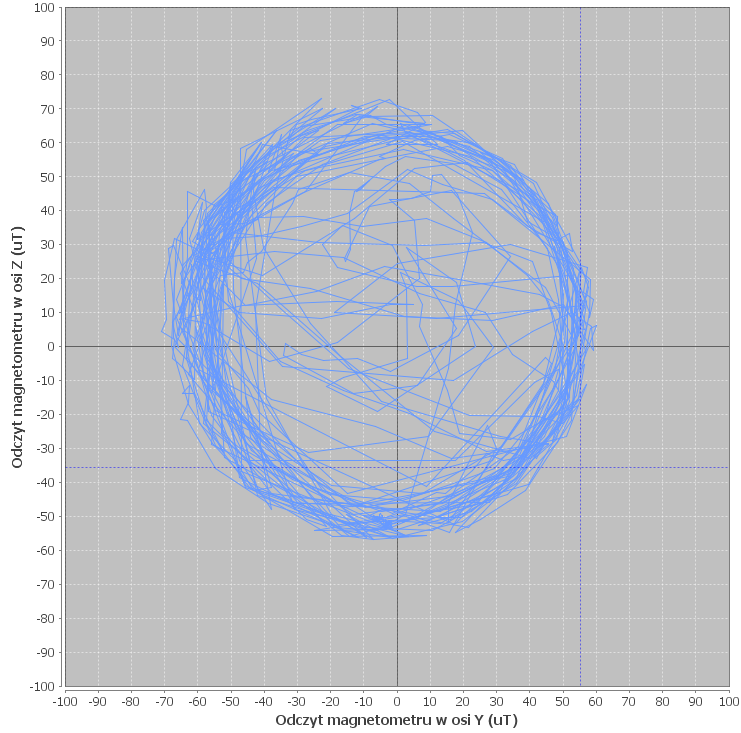
\includegraphics[width=0.5\textwidth]{Rysunki/Rozdzial03/Magnetometr_skalibrowany_hardiron_YZ.png}
    \caption{Odczyty dla skalibrowanego magnetometru}
    \label{Magnetometr skalibrowany}
\end{figure}

%----------------------------------------------------------------------------------------------------------------
\chapter{Wybrane metody fuzji sygnałów}
\label{chap:wybrane}

Z racji tego, że każdy z omówionych czujników ruchu posiada swoje niedoskonałości, takie jak dryf kątów obrotu obliczonych na podstawie odczytów z żyroskopu, brak odporności na szybkozmienne zakłócenia akcelerometru oraz wpływ ferromagnetyków na odczyty magnetometru, konieczna jest fuzja pochodzących z czujników sygnałów, za pomocą dostępnych algorytmów, w celu osiągnięcia zadowalającego rezultatu obliczonych rotacji wokół osi. Za zadowalający rezultat, uznaje się brak dryfu, brak zakłóceń szybkozmiennych oraz skompensowane stałe zakłócenia pochodzące z ferromagnetyków w pobliżu czujnika. W tym celu zaimplementowano i przetestowano trzy znane algorytmy wykorzystywane w zakresie fuzji sygnałów:
\begin{itemize}
    \item Filtr komplementarny
    \item Filtr Kalmana
    \item Filtr Madgwicka
\end{itemize}

%----------------------------------------------------------------------------------------------------------------
\section{Filtr komplementarny}

Jednym z łatwiejszych w implementacji filtrów używanych do fuzji dwóch lub większej ilości sygnałów, jest filtr komplementarny. Zasada działania tego filtra opiera się o filtr dolno i górno przepustowy, za pomocą których eliminujemy zakłócenia wolno i szybko zmienne. Przedstawiony poniżej algorytm filtra komplementarnego opracowano w oparciu o artykuł \cite{Komplementarny2}. Schemat filtra znajduje się na rysunku \ref{filtr komplementarny}.

\begin{figure}[h!]
    \centering
    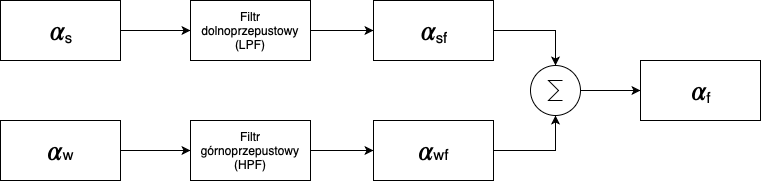
\includegraphics[width=0.75\textwidth]{Rysunki/Rozdzial04/Filtr_komplementarny.png}
    \caption{Schemat blokowy filtra komplementarnego}
    \label{filtr komplementarny}
\end{figure}

Przyjęto oznaczenia:

$\alpha_s$ -- pomiar kąta obarczony szybko-zmiennymi zakłóceniami

$\alpha_{sf}$ -- pomiar kąta pozbawiony szybko-zmiennych zakłóceń

$\alpha_w$ -- pomiar kąta obarczony wolno-zmiennymi zakłóceniami

$\alpha_{wf}$ -- pomiar kąta pozbawiony wolno-zmiennych zakłóceń

$\alpha_f$ -- kąt po odfiltrowaniu zakłóceń

%----------------------------------------------------------------------------------------------------------------
\subsection{Filtr dolnoprzepustowy}

Za pomocą filtra dolnoprzepustowego eliminujemy zakłócenia szybko zmienne (charakterystyczne, np. dla akcelerometru lub magnetometru) powyżej częstotliwości granicznej, która powiązana jest ze stałą czasową w następujący sposób
$$
    f_{gr} = \frac{1}{2\pi RC} = \frac{1}{2\pi\tau}
$$

Dyskretny wzór na sygnał wyjściowy z filtra dolnoprzepustowego, można wyprowadzić w oparciu o model obwodu RC, w którym iloczyn wartości R i C stanowi wartość stałej czasowej filtra $\tau$.

\begin{figure}[htb!]
    \centering
    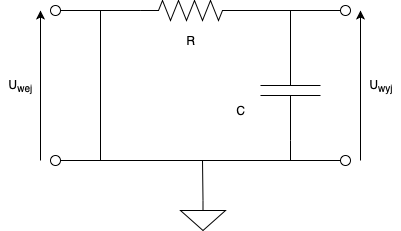
\includegraphics[width=0.5\textwidth]{Rysunki/Rozdzial04/FIltr_dolnoprzepustowy.png}
    \caption{Filtr dolnoprzepustowy RC}
    \label{filtr dp}
\end{figure}

Transmitancja filtra dolnoprzepustowego
$$
    \frac{U_{wyj}}{U_{wej}} = \frac{1}{RCs + 1} = \frac{1}{\tau s + 1}
$$
Na podstawie transmitancji otrzymujemy wzór na wartość napięcia wejściowego filtra
$$
     U_{wej} = RC\Dot{U}_{wyj} + U_{wyj} = \tau \Dot{U}_{wyj} + U_{wyj}
$$
Następnie wprowadzając oznaczenia $x = U_{wej}$ oraz $y = U_{wyj}$ i przekształcając wzór względem wartości wyjściowej $y$ otrzymujemy wzór na dyskretną wartość na wyjściu filtra 
\begin{equation}
    y(t) = x(t)\frac{\Delta t}{\tau + \Delta t} + y(t-1)\frac{\tau}{\tau + \Delta t} = \gamma x(t) + (1 - \gamma)y(t-1)
    \label{wyjscie dp}
\end{equation}
dla którego
$$
    0 \leq \gamma \leq 1,
    \quad
    \tau = \Delta t\left(\frac{1 - \gamma}{\gamma}\right)
$$

%----------------------------------------------------------------------------------------------------------------
\subsection{Filtr górnoprzepustowy}

Jeśli mamy do czynienia z zakłóceniami wolno zmiennymi (np. w przypadku żyroskopu) korzysta się z filtra górnoprzepustowego, odcinającego zakłócenia poniżej częstotliwości granicznej, która związana jest ze stałą czasową w taki sam sposób, jak w przypadku filtra dolnoprzepustowego.
$$
$$

\begin{figure}[htb!]
    \centering
    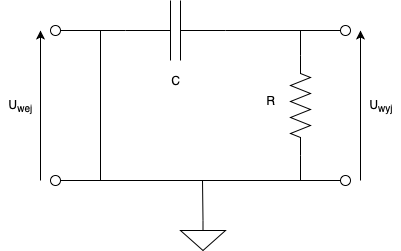
\includegraphics[width=0.5\textwidth]{Rysunki/Rozdzial04/FIltr_gornoprzepustowy.png}
    \caption{Filtr górnoprzepustowy CR}
    \label{filtr gp}
\end{figure}

Transmitancja filtra górnoprzepustowego
$$
    \frac{U_{wyj}}{U_{wej}} = \frac{RCs}{RCs + 1} = \frac{\tau s}{\tau s + 1}
$$
Postępując analogicznie jak w przypadku filtra dolnoprzepustowego otrzymujemy zależności pomiędzy napięciem wejściowym, a wyjściowym
$$
   RC\Dot{U}_{wyj} + U_{wyj} = RC\Dot{U}_{wej} \Rightarrow \tau\Dot{U}_{wyj} + U_{wyj} = \tau\Dot{U}_{wej} 
$$
Wprowadzając oznaczenia, jak w przypadku filtra dolnoprzepustowego otrzymujemy wzór na dyskretną wartość wyjściową
\begin{equation}
    y(t) = \tau\frac{x(t) - x(t-1)}{\Delta t} - \frac{y(t) - y(t-1)}{\Delta t}  = \beta y(t-1) + \beta(x(t) - x(t-1))
    \label{wyjscie gp}
\end{equation}
dla której
$$
    0 \leq \beta \leq 1,
    \quad
    \tau = \Delta t\left(\frac{\beta}{1 - \beta}\right)
$$

%----------------------------------------------------------------------------------------------------------------
\subsection{Równanie filtra komplementarnego}
Parametry $\gamma$ oraz $\beta$ muszą spełniać zasadę komplementarności
$$
    \gamma + \beta = 1
$$
co wynika z natury samego filtra.

Podstawiając wartości wejściowe dla filtra do wzorów ogólnych (\ref{wyjscie dp}) oraz (\ref{wyjscie gp}) otrzymujemy dwa równania
$$
    \begin{array}{cc}
        \alpha_{sf}(t) = \alpha_{s}(t) + (1 - \gamma)\alpha_{sf}(t-1) \\ \\
        \alpha_{wf}(t) = \beta \alpha_{wf}(t-1) + \beta(\alpha_w(t) - \alpha_w(t-1))
    \end{array}
$$
które po zsumowaniu dają równanie filtra komplementarnego
$$
    \begin{array}{cc}
        \alpha_f(t) = \alpha_{sf}(t) + \alpha_{wf}(t) = \alpha_{s}(t) + (1 - \gamma)\alpha_{sf}(t-1) + \beta \alpha_{wf}(t-1) + \beta(\alpha_w(t) - \alpha_w(t-1))
    \end{array}
$$
Po podstawieniu $\gamma = 1 - \beta$ i uproszczeniu wzoru otrzymujemy ostateczną postać równania filtra komplementarnego
\begin{equation}
    \alpha_f(t) = \beta(\alpha_w(t) - \alpha_w(t-1) + \alpha_f(t-1)) + (1 - \beta)\alpha_s(t)
\end{equation}
gdzie
$\beta$ -- parametr dostrajający filtr wyznaczany eksperymentalnie

%----------------------------------------------------------------------------------------------------------------
\section{Filtr Kalmana}

Celem przedstawionej tutaj implementacji filtra Kalmana, jest uzyskanie odchylenia kątowego, w oparciu o wartości odchylenia kątowego obliczonego na podstawie pomiarów pochodzących z akcelerometru, oraz prędkości kątowej zmierzonej przez żyroskop. Wartość na wyjściu filtra powinna być pozbawiona zakłóceń szybko oraz wolno zmiennych, które wynikają z zasady działania oraz sposobu obliczeń dla akcelerometru i żyroskopu. Zmienne wejściowe oraz wyjściowe dla filtra Kalmana przedstawiono na rysunku \ref{Kalman idea}. Parametrami, które decydują o charakterystyce sygnału wyjściowego są: $q$ -- wariancja procesu, oraz $r$ -- wariancja pomiaru. Są to parametry wyznaczane eksperymentalnie. Dokładniejszy opis i zasadę działania algorytmu, można znaleźć w pracy \cite{Kalman} poświęconej w pełni filtrowi Kalmana, na podstawie której powstał poniższy opis algorytmu.

\begin{figure}[h!]
    \centering
    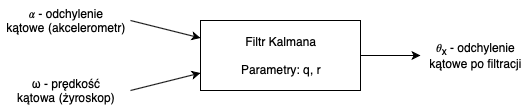
\includegraphics[width=0.75\textwidth]{Rysunki/Rozdzial04/Kalman_idea.png}
    \caption{Zmienne wejściowe oraz wyjściowe dla filtra Kalmana}
    \label{Kalman idea}
\end{figure}

Dane wejściowe podawane są w następujących jednostkach
\begin{itemize}
    \item $\alpha (^o)$
    \item $\omega (^0/s)$
\end{itemize}

Do działania filtru konieczne jest zamodelowanie obiektu w postaci równań stanu. W tym celu zaproponowano równanie opisujące system
$$
    \theta_x(t) = \theta_x(t-1) + (\omega_x(t-1) - \zeta_x)\Delta t
$$
co można rozpisać na następujące równania
\begin{equation}
    \begin{array}{l}
        \theta_x(t) = \theta_x(t-1) - \zeta_x(t-1)\Delta t + \omega\Delta t \\
        \omega_x(t) = \omega - \zeta_x(t-1) \\
        \zeta_x(t) = \zeta_x(t-1)
    \end{array}
    \label{Rownania obiektu}
\end{equation}
gdzie wartości na wyjściu systemu to odpowiednio
\begin{itemize}
    \item $\theta_x$ -- wartość odchylenia kątowego 
    \item $\omega_x$ -- wartość prędkości kątowej 
    \item $\zeta_x$ -- wartość błędu żyroskopu (dryf)
\end{itemize}

Mając równania systemu w takiej postaci, możemy zapisać je w postaci macierzowej, czyli sformułować równania stanu obiektu.
%----------------------------------------------------------------------------------------------------------------
\subsection{Równanie stanu obiektu}
Równanie stanu sformułowane na podstawie równań (\ref{Rownania obiektu})
$$
    x(t) = Ax(t-1) + Bu
$$
gdzie
$$
    \mathbf{A} =
    \left[
    \begin{array}{ccc}
        1 & 0 & -\Delta t \\
        0 & 0 & -1 \\
        0 & 0 & 1
    \end{array}
    \right]
    \quad
    \mathbf{B} = 
    \left[
    \begin{array}{c}
        \Delta t \\
        1 \\
        0
    \end{array}
    \right]
$$
%
Wektor stanu
$$
    \mathbf{x} = 
    \left[
    \begin{array}{c}
        \theta_x \\
        \omega_x \\
        \zeta_x
    \end{array}
    \right]
$$
%
W tym przypadku sterowaniem systemu jest prędkość kątowa odczytana z żyroskopu
$$
    \mathbf{u} = \omega
$$
%
Z racji tego, że na wyjściu systemu istotne dla nas jest aktualne odfiltrowane odchylenie kątowe $\theta_x$ przechowywane w wektorze stanu po aktualizacji, macierz wyjścia przyjmuje postać
$$
    \mathbf{C} = 
    \left[
    \begin{array}{ccc}
        1 & 0 & 0
    \end{array}
    \right]
$$
%
Macierz kowariancji pomiaru, w pierwszej iteracji algorytmu przyjmuje postać macierzy diagonalnej, mającej na swej diagonali wartości wariancji pomiaru
$$
    \mathbf{P} = 
    \left[
    \begin{array}{ccc}
        r & 0 & 0 \\
        0 & r & 0 \\
        0 & 0 & r
    \end{array}
    \right]
$$
%
Macierz kowariancji procesu, w pierwszej iteracji algorytmu przyjmuje postać macierzy diagonalnej, mającej na swej diagonali wartości wariancji procesu
$$
    \mathbf{Q} = 
    \left[
    \begin{array}{ccc}
        q & 0 & 0 \\
        0 & q & 0 \\
        0 & 0 & q
    \end{array}
    \right]
$$
%
Macierz szumu akcelerometru jest jedno wymiarowa i przyjmuje wartość wariancji pomiaru
$$
    \mathbf{R} = r
$$

%----------------------------------------------------------------------------------------------------------------
\subsection{Równania filtru Kalmana}

Faza predykcji
\begin{enumerate}
    \item prognoza stanu: $$x(t) = Ax(t-1) + B \omega$$
    \item prognoza błędu kowariancji: $$P(t) = AP(t-1)A^T+Q$$
\end{enumerate}
%
Faza korekcji
\begin{enumerate}
    \item wzmocnienie filtra Kalmana: $$K(t) = P(t)H^TH(HP(t)H^T+R)^{-1}$$
    \item aktualizacja estymacji w oparciu o rzeczywisty pomiar: $$x(t) = x(t) + K(t)(\alpha - Hx(t))$$
    \item aktualizacja błędu kowariancji: $$P(t) = (1 - K(t)H)P(t)$$
\end{enumerate}

W każdej iteracji działania algorytmu, aktualny kąt wychylenia $\theta_x$ znajduje się w zaktualizowanym wektorze stanu. Jest to wartość wyjściowa filtra pozbawiona zakłóceń.

%----------------------------------------------------------------------------------------------------------------
\section{Filtr Madgwicka}

W 2010 roku S.O Madgwick opublikował raport \cite{Madgwick2010AnEO} dotyczący opracowanego przez siebie algorytmu do uzyskiwania orientacji w przestrzeni czujników MARG. Przewagą jaką ma owy filtr nad innymi znanymi filtrami jest to, że nie wymaga on kalibracji magnetometru. Algorytm samodzielnie radzi sobie z odkształceniami ,,hard iron'' oraz ,,soft iron''. Drugą dużą zaletą jest odporność na tzw. efekt ,,gimbal lock'', który jest poważną wadą przy opisie orientacji za pomocą kątów RPY oraz Eulera. Objawia się on maksymalnym zakresem dla kąta Pitch wynoszącym $<-90^o, 90^o>$, co wynika z maksymalnej oraz minimalnej wartości jaką przyjmuje funkcja arcus sinus.

Inne zalety jakie w swoim raporcie wymienia autor to m.in niski koszt obliczeniowy, dzięki czemu algorytm z powodzeniem można implementować na słabszych mikroprocesorach oraz wysoka skuteczność przy niskich częstotliwościach próbkowania czujników, np. 10Hz.

\begin{figure}[h!]
    \centering
    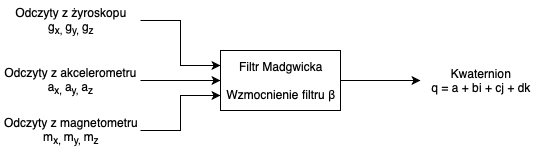
\includegraphics[width=0.75\textwidth]{Rysunki/Rozdzial04/Madgwick_idea.png}
    \caption{Zmienne wejściowe oraz wyjściowe dla filtra Madgwicka}
    \label{Madgwick idea}
\end{figure}

Dane wejściowe podawane są w następujących jednostkach
\begin{itemize}
    \item $g_x, g_y, g_z (rad/s)$
    \item $a_x, a_y, a_z (g)$
    \item $m_x, m_y, m_z (\mu T)$
\end{itemize}

Do matematycznego opisu orientacji w przestrzeni algorytm wykorzystuje kwaterniony, które z powodzeniem można przeliczyć na kąty RPY
$$
    \begin{array}{l}
        Roll = arctan\left(\frac{2(ab + cd)}{1 - 2(b^2 + c^2)}\right) \\ \\
        Pitch = -arcsin(2(ac + db)) \\ \\
        Yaw = arctan\left(\frac{2(ad + bc)}{1 - 2(c^2 + d^2)}\right) 
    \end{array}
$$

%----------------------------------------------------------------------------------------------------------------
\subsection{Poszczególne etapy działania algorytmu}

\begin{enumerate}
    \item Wyznaczenie szybkości zmiany orientacji kwaternionu na podstawie wektora prędkości kątowych
    $$
        _E^S \Dot{q}_{\omega,t} = \frac{1}{2} \ _E^S \hat{q}_{est,t-1} \tens \ \omega
    $$
    gdzie \\
    $ \tens \ $ -- iloczyn tensorowy \\
    $ _E^S \hat{q}_{est,t-1} $ -- znormalizowany kwaternion z poprzedniej iteracji\\
    $ \omega $ -- wektor prędkości kątowych
    \item Wyznaczenie kierunku referencyjnego pola magnetycznego oraz współczynnika korygującego zaburzenia pola magnetycznego
    $$
        \begin{array}{cc}
            ^E \hat{h_t} = _E^S \hat{q} \tens \ \hat{m_t} \tens \ \ _E^S \hat{q}^{*} = [0 \quad h_x \quad h_y \quad h_z] \\ \\
            ^E \hat{b_t} = [0 \quad \sqrt{h_x^2 + h_y^2} \quad 0 \quad h_z]
        \end{array}
    $$
    gdzie \\
    $ \hat{m_t} $ -- znormalizowany wektor pomiarów z magnetometru\\
    $ _E^S \hat{q}^{*} = _S^E \hat{q} $ -- sprzężenie kwaternionu orientacji
    \item Znalezienie minimum lokalnego funkcji celu
    $$
        f(_E^S \hat{q}, \hat{d}, \hat{s}) = _E^S \hat{q}^{*} \tens \ \hat{d} \tens \ \ _E^S \hat{q} - \hat{s}
    $$
    metodą gradientu prostego w wyniku, które otrzymujemy błąd zmiany orientacji w danym zakresie czasu
    $$
        _E^S \Dot{\hat{q}}_{s,t}
    $$
    który pozwala na wyznaczenie estymaty wartości szybkości zmiany orientacji kwaternionu
    $$
        _E^S \Dot{q}_{est,t} = _E^S \Dot{q}_{\omega,t} - \beta _E^S \Dot{\hat{q}}_{s,t}
    $$
    \item Całkując szybkość zmiany orientacji kwaternionu po czasie otrzymujemy aktualną orientację kwaternionu 
    $$
        _E^S q_{est,t} = _E^S q_{est,t-1} + _E^S \Dot{q}_{est,t} \Delta t
    $$
    którą możemy wykorzystać do obliczenia kątów RPY, lub pozostawić w postaci kwaternionu jeśli bazujemy na takiej metodzie określania orientacji w przestrzeni, jednak jest ona dosyć nieintuicyjna i mało czytelna na pierwszy rzut oka. 
    
\end{enumerate}

%----------------------------------------------------------------------------------------------------------------
\section{Testy symulacyjne}

Testy opisanych wcześniej trzech algorytmów przeprowadzone zostały w środowisku \texttt{Matlab Simulink}, z wykorzystaniem danych pochodzących z rzeczywistego modułu MARG MPU9250. Dane zostały wprowadzone w następujących jednostkach
\begin{itemize}
    \item Żyroskop -- prędkość kątowa ($^o/s$) 
    \item Akcelerometr -- przyspieszenie ($g$)
    \item Magnetometr -- indukcja pola magnetycznego ($\mu T$) 
\end{itemize}

Przed zapisaniem danych czujnik został skalibrowany, o czym więcej w kolejnym rozdziale \ref{chap:budowa} dotyczącym budowy robota balansującego. Wczytane dane zaprezentowane zostały na rysunku \ref{MARG sygnaly}
\begin{figure}[h!]
    \centering
    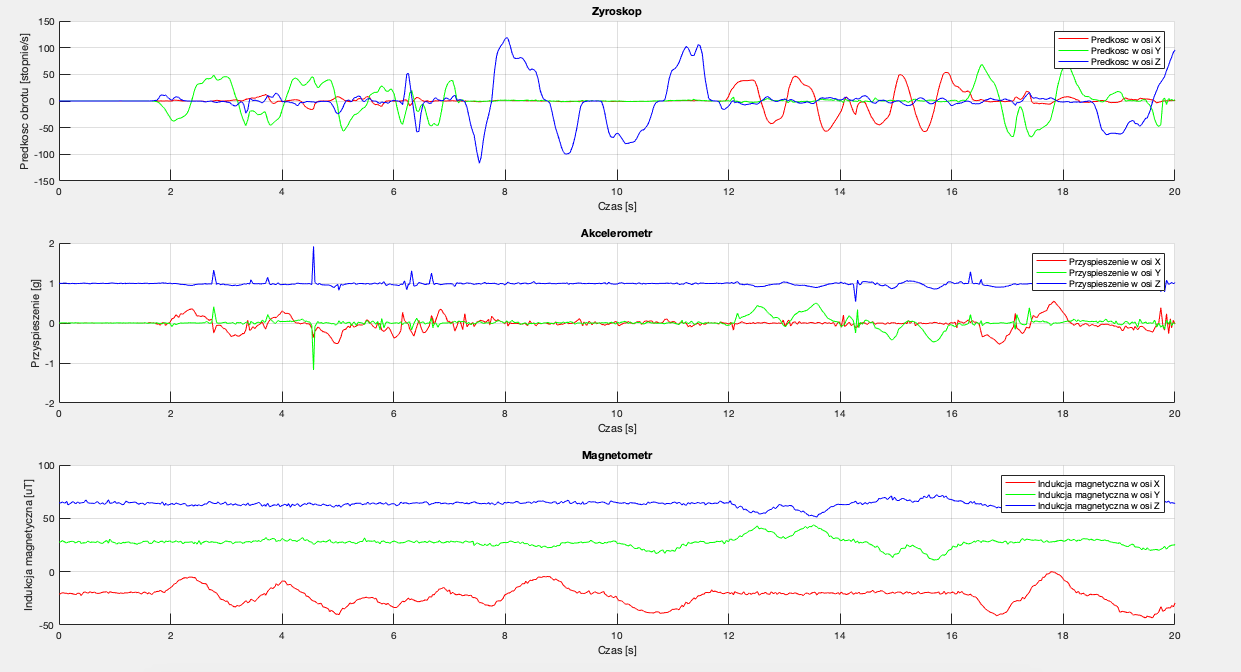
\includegraphics[width=1\textwidth]{Rysunki/Rozdzial04/MARG_sygnaly.png}
    \caption{Sygnały z modułu wykorzystane podczas symulacji}
    \label{MARG sygnaly}
\end{figure}

\newpage
%----------------------------------------------------------------------------------------------------------------
\subsection{Filtr komplementarny}

Do implementacji filtra komplementarnego, wykorzystano bloczki \texttt{Transfer Fcn}, do których zostały wprowadzone odpowiednie transmitancje, oraz stała czasowa wczytywana ze skryptu.
\begin{figure}[h!]
    \centering
    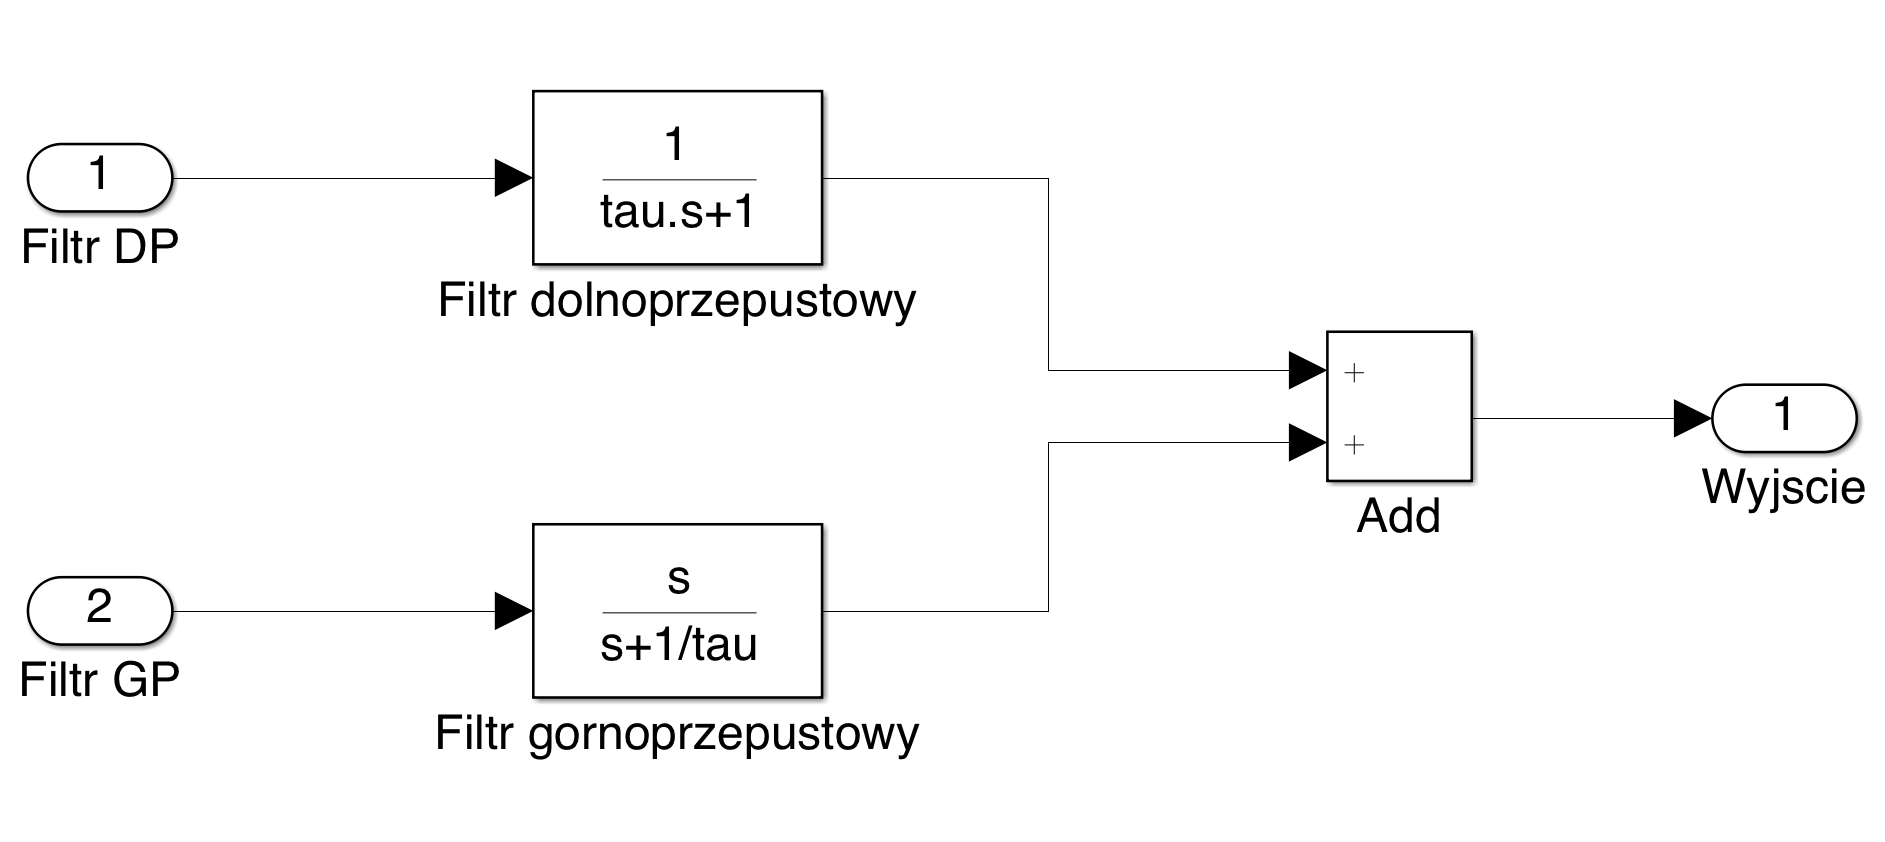
\includegraphics[width=0.75\textwidth]{Rysunki/Rozdzial04/Filtr_komplementarny_implementacja.png}
    \caption{Implementacja filtra komplementarnego}
    \label{Komplementarny implementacja}
\end{figure}

Filtr komplementarny wykorzystano do uzyskania rotacji w trzech osiach. Rotację w osiach X i Y uzyskano na podstawie pomiarów z akcelerometru i żyroskopu, a rotację w okół osi Z na podstawie pomiarów z magnetometru i żyroskopu

\newpage
\begin{figure}[h!]
    \centering
    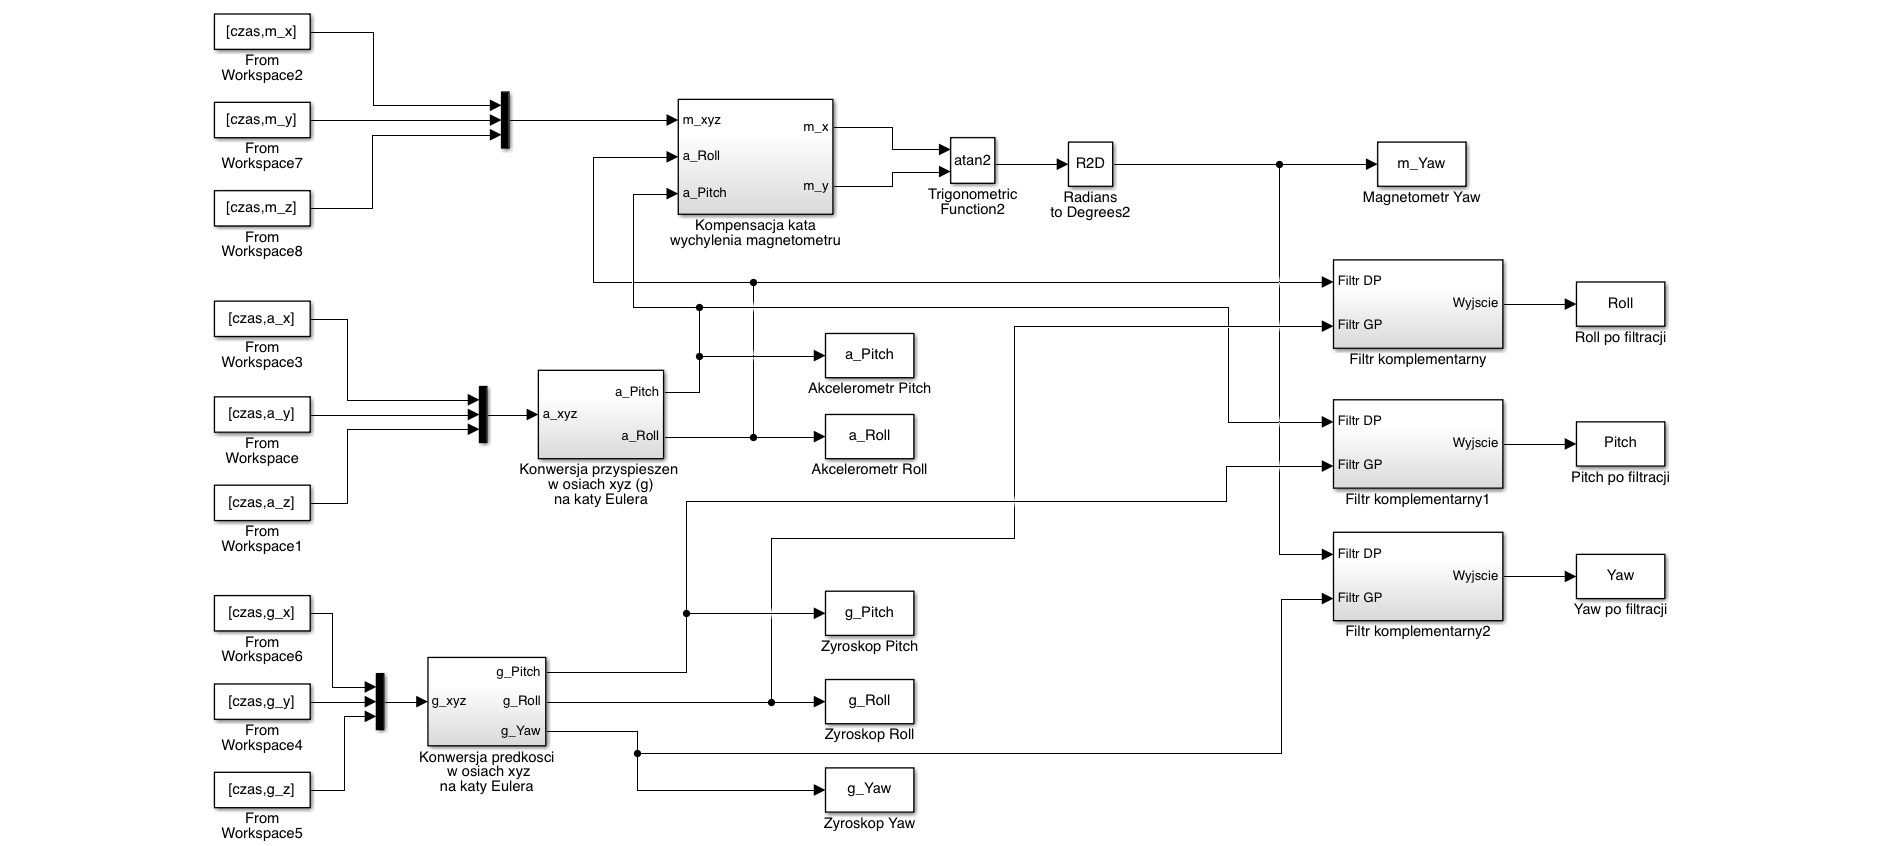
\includegraphics[width=1\textwidth]{Rysunki/Rozdzial04/Filtr_komplementarny_struktura_png.png}
    \caption{Wykorzystanie filtra komplementarnego dla sygnałów z akcelerometru, żyroskopu i magnetometru}
    \label{Komplementarny struktura}
\end{figure}

 Na rysunku \ref{Komplementarny przed} widać, że akcelerometr i magnetometr obarczony jest szybkozmiennymi zakłóceniami, a żyroskop wolnozmiennymi.
\begin{figure}[h!]
    \centering
    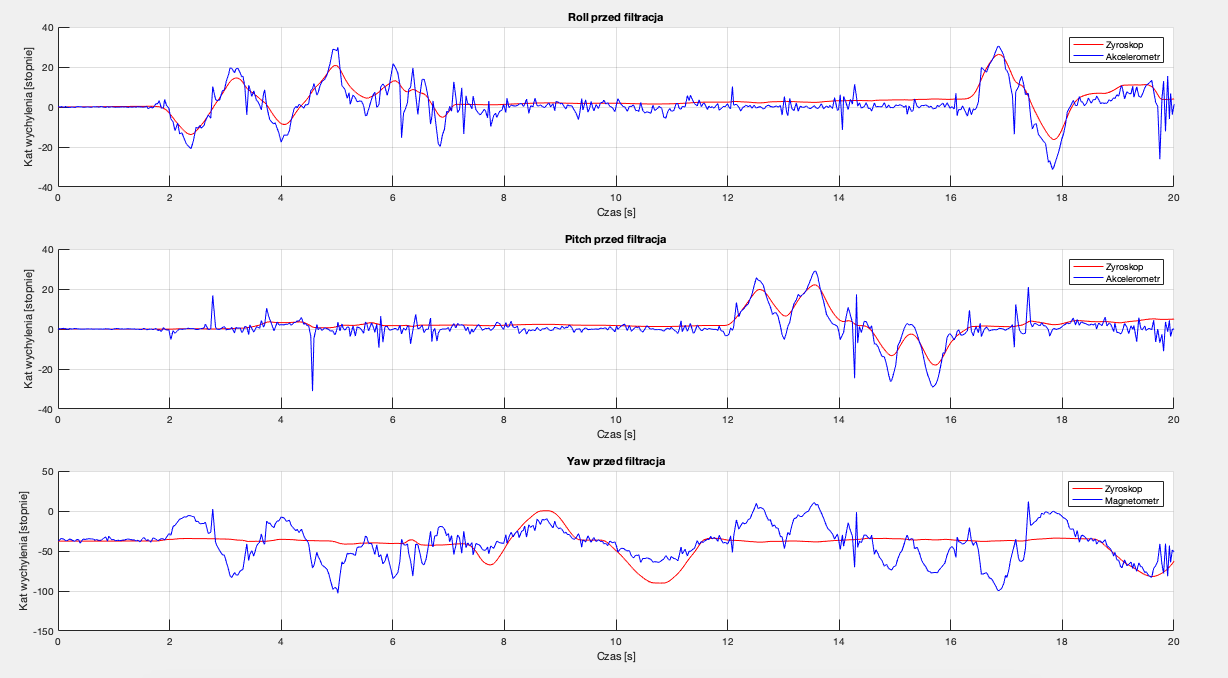
\includegraphics[width=1\textwidth]{Rysunki/Rozdzial04/Filtr_komplementarny_przed.png}
    \caption{Sygnały wejściowe dla filtra komplementarnego}
    \label{Komplementarny przed}
\end{figure}

W trakcie testowania algorytmu zdecydowano się dobrać trzy wartości stałej czasowej
$$
    \begin{array}{ccc}
        \tau_1 = 1 & \tau_2 = 0.01 & \tau_3 = 0.0001
    \end{array}
$$
które odpowiadają odpowiednio parametrowi filtra przy czasie próbkowania $\Delta t = 0.01s$
$$
    \begin{array}{ccc}
        \beta_1 \approx 0.99 & \beta_2 = 0.5 & \beta_3 \approx 0.009
    \end{array}
$$

\begin{figure}[h!]
    \centering
    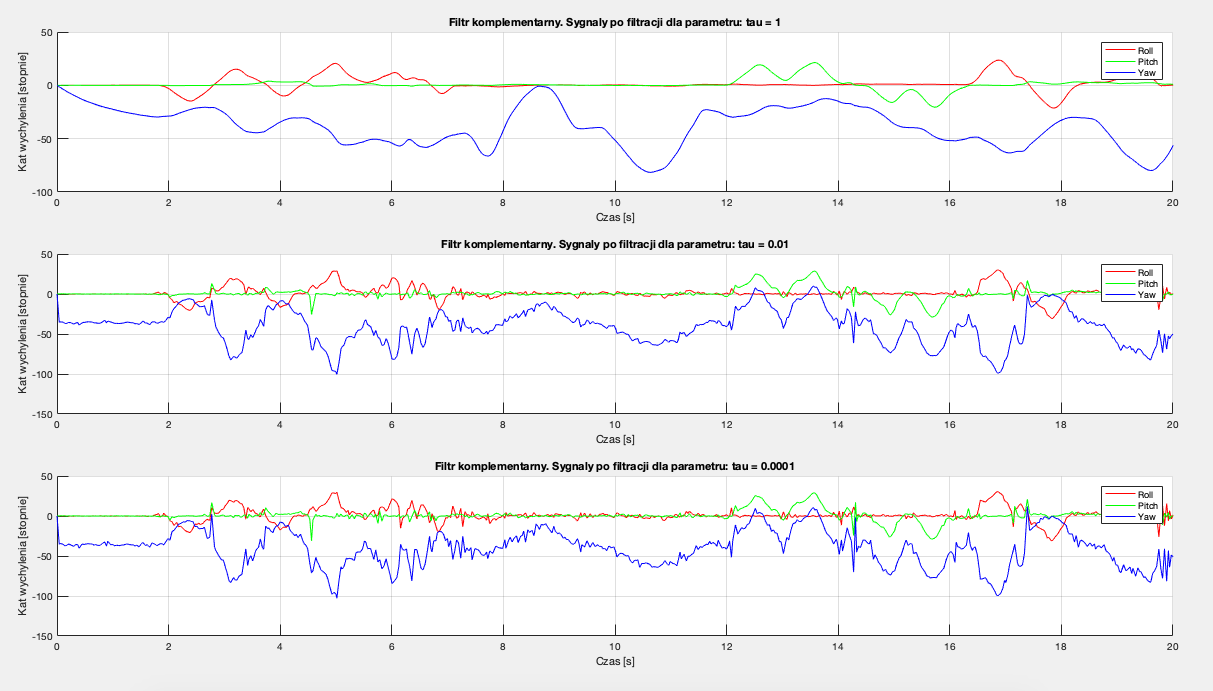
\includegraphics[width=1\textwidth]{Rysunki/Rozdzial04/Filtr_komplementarny_po.png}
    \caption{Sygnały wyjściowe dla filtra komplementarnego}
    \label{Komplementarny po}
\end{figure}

Stała czasowa decyduje o tym, jaką część z ostatecznej wartości na wyjściu filtra stanowi pomiar z akcelerometru lub magnetometru, a jaką pomiar z żyroskopu. Stąd wywnioskowano, że im większa stała czasowa tym większy udział w ostatecznym wyniku ma pomiar z żyroskopu (mniej widocznych zakłóceń szybkozmiennych).
%----------------------------------------------------------------------------------------------------------------
\subsection{Filtr Kalmana}

Sygnałami wejściowymi dla filtra Kalmana są obarczone zakłóceniami szybkozmiennymi kąty obliczone na podstawie odczytów z akcelerometru oraz prędkości kątowe odczytane za pomocą żyroskopu, rysunek \ref{Kalman przed}

\begin{figure}[h!]
    \centering
    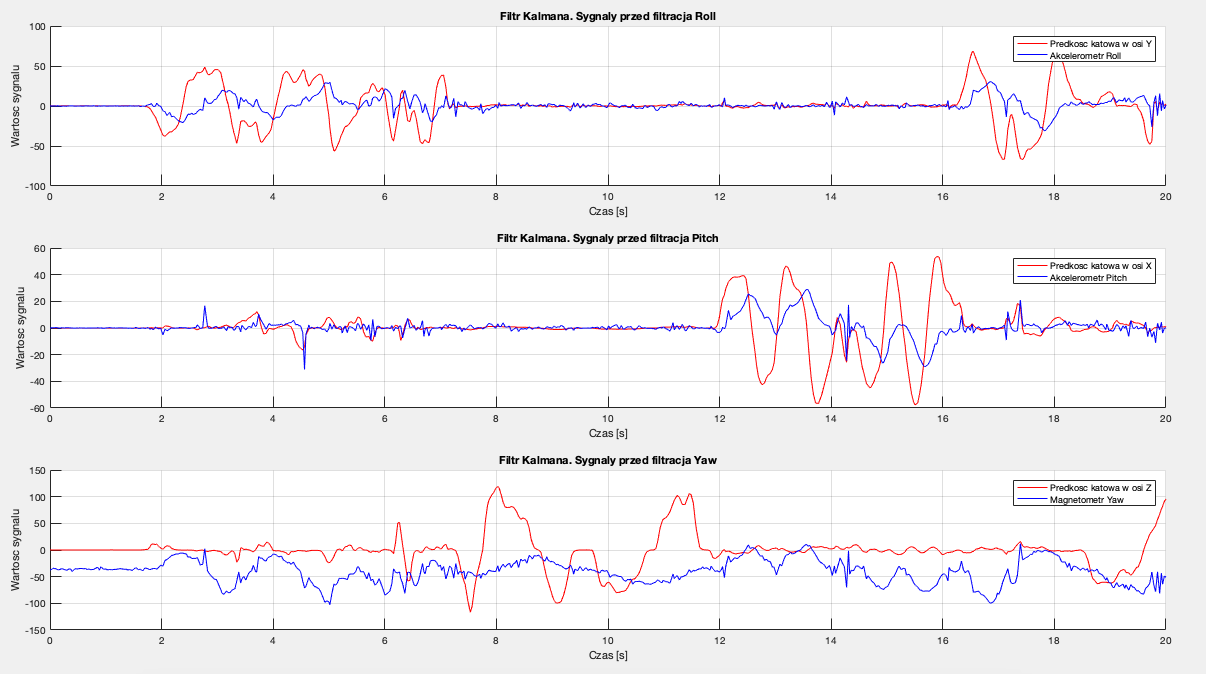
\includegraphics[width=1\textwidth]{Rysunki/Rozdzial04/Filtr_Kalmana_przed.png}
    \caption{Sygnały wejściowe dla filtra Kalmana}
    \label{Kalman przed}
\end{figure}

W celach eksperymentalnych spróbowano zastosować kąty obliczone na podstawie odczytów z magnetometru zamiast akcelerometru do wyznaczenia obrotu wokół osi Z. Z powodzeniem uzyskano wyniki zbliżone do filtra komplementarnego. Dodatkowo przetestowano algorytm dla trzech par parametrów
$$
    \begin{array}{ll}
        r_1 = 1000 & q_1 = 10000 \\
        r_2 = 1 & q_2 = 1 \\
        r_3 = 0.0001 & q_3 = 10 
    \end{array}
$$
\begin{figure}[h!]
    \centering
    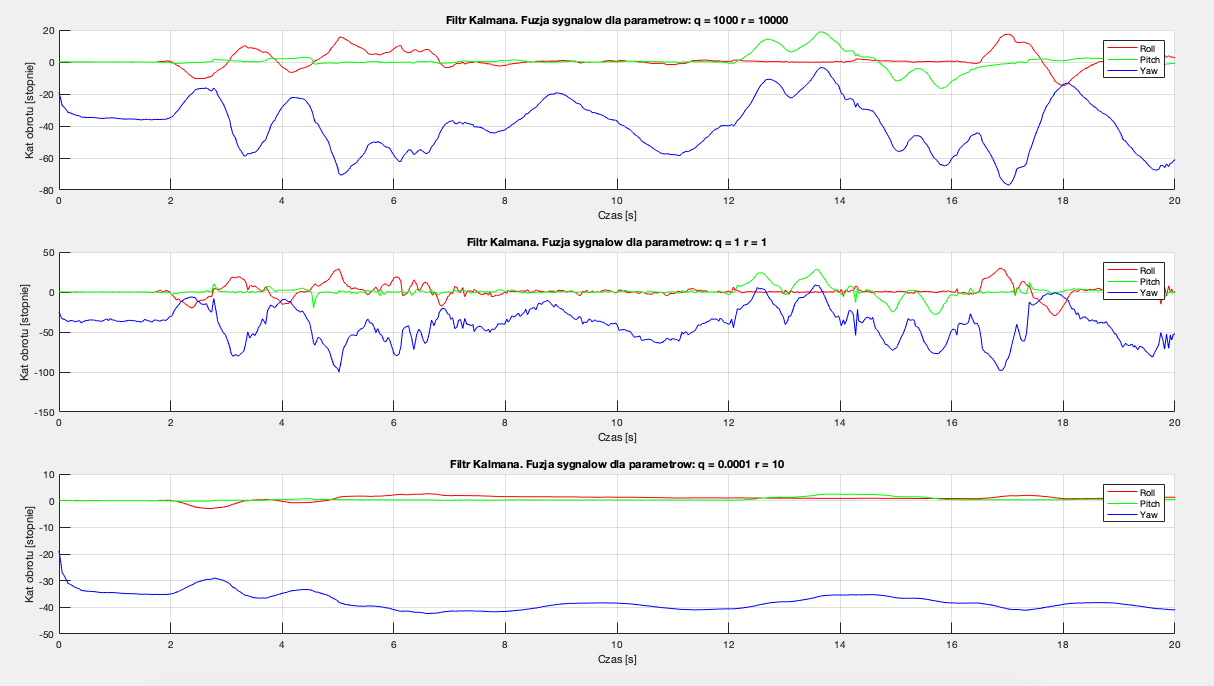
\includegraphics[width=1\textwidth]{Rysunki/Rozdzial04/Filtr_Kalmana_po.png}
    \caption{Sygnały wyjściowe dla filtra Kalmana}
    \label{Kalman po}
\end{figure}

%----------------------------------------------------------------------------------------------------------------
\subsection{Filtr Madgwicka}

\begin{figure}[h!]
    \centering
    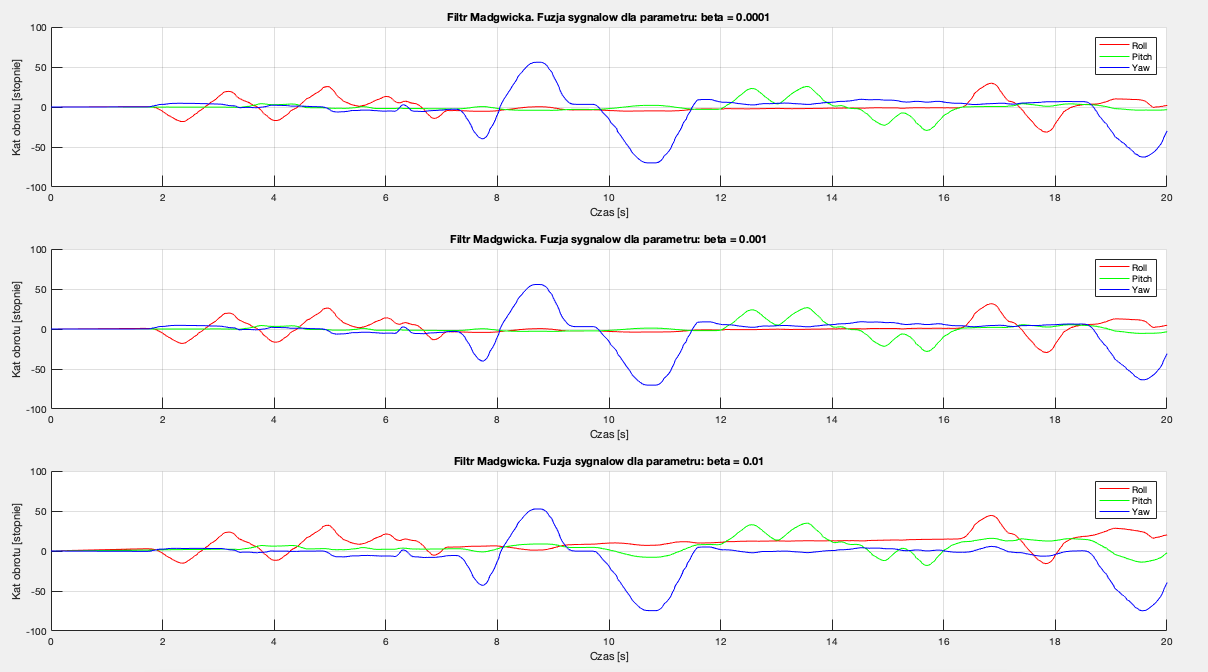
\includegraphics[width=1\textwidth]{Rysunki/Rozdzial04/Filtr_Madgwicka_po.png}
    \caption{Sygnały wyjściowe dla filtra Madgwicka}
    \label{Madgwick po}
\end{figure}

%----------------------------------------------------------------------------------------------------------------
\subsection{Porównanie filtrów}

W teście wykorzystano następujące parametry filtrów
\begin{table}[h!]
    \centering
    \begin{tabular}{|c|c|c|}
        \hline
        F.komplementarny & F.Kalmana & F.Madgwicka \\
        \hline
        $\tau = 0.1$ & $r = 10000$, $q = 1000$ & $\beta = 0.001$ \\
        \hline
    \end{tabular}
    
     \caption{Parametry filtrów przyjęte podczas porównania}
\end{table}

Dla kątów Roll oraz Pitch algorytmy działają podobnie, jednak dla kąta Yaw widać znaczną przewagę filtra Madgwicka, który zdecydowanie lepiej poradził sobie z zakłóceniami szybkozmiennymi pochodzącymi od magnetometru. Wyraźnie widoczne jest to między sekundą 0-7 oraz 12-17 na wykresie \ref{Porownanie}. Kiedy chciano poprawić działanie filtra komplementarnego i Kalmana dla kąta Yaw, tak aby osiągnąć wynik zbliżony do tego dla filtra Madgwicka, nie przyniosło to zadowalających rezultatów. Owszem zakłócenia zostały zniwelowane, ale sygnały zaczęły znacząco odbiegać od rzeczywistości. 

\begin{figure}[h!]
    \centering
    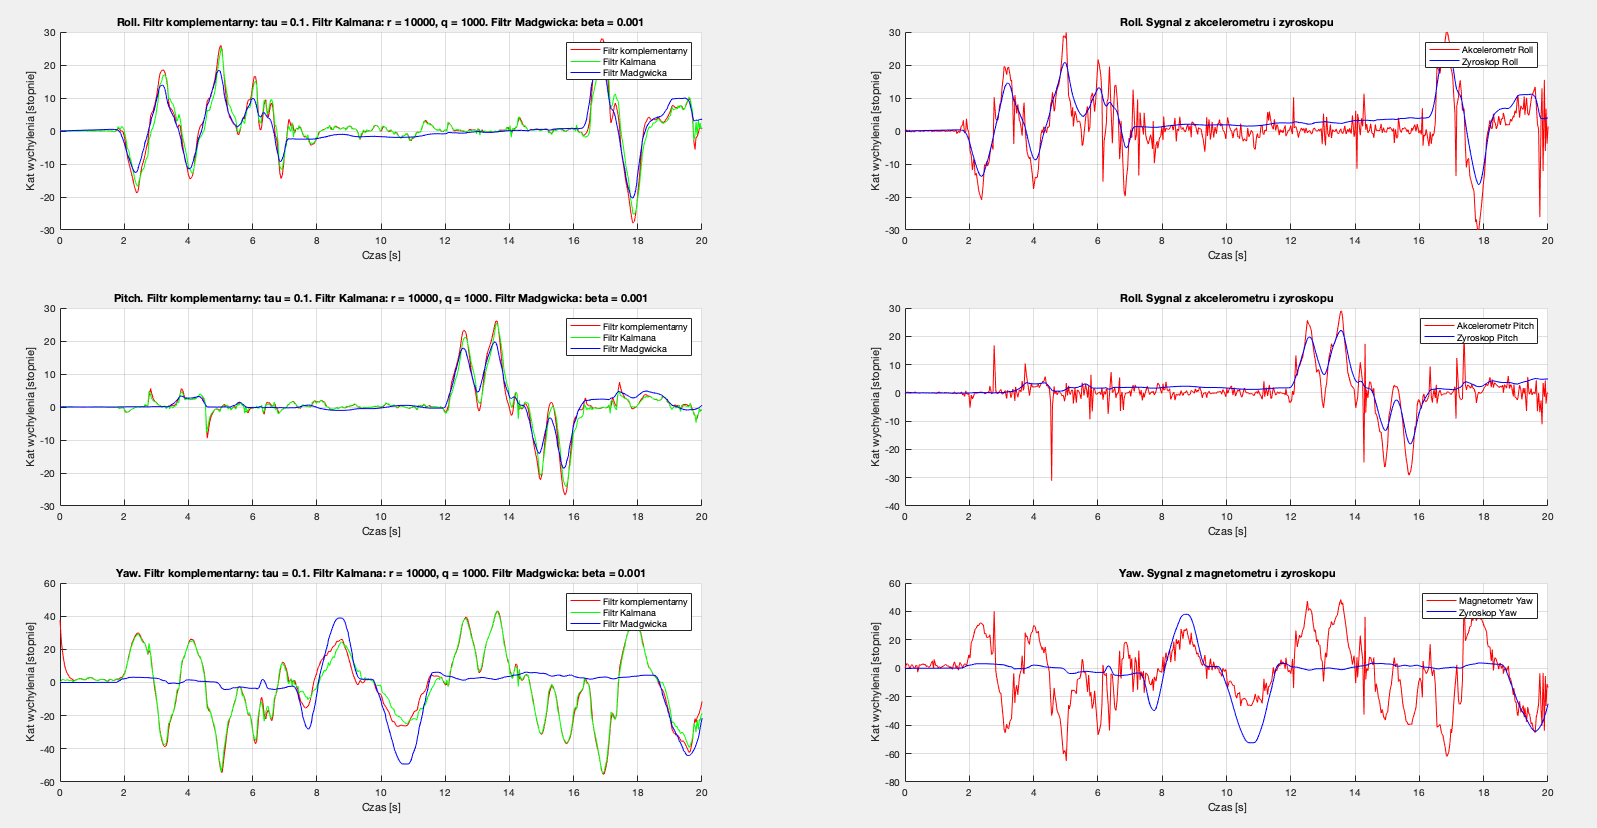
\includegraphics[width=1\textwidth]{Rysunki/Rozdzial04/Porownanie.png}
    \caption{Wykresy zbiorcze dla wszystkich filtrów}
    \label{Porownanie}
\end{figure}

Warto też dodać, że wartość początkowa kąta obliczanego na podstawie odczytów z żyroskopu wynosi 0. Tak aby porównanie działania filtrów było miarodajne, należy przesunąć kąt obliczany na podstawie odczytów z żyroskopu o pewną wartość względem pomiarów obliczanych na podstawie odczytów z magnetometru, tak aby w chwili $t = 0$ oba wykresy miały tą samą wartość.
\chapter{Budowa dwukołowego robota balansującego}
\label{chap:budowa}

W celu przetestowania zaimplementowanych metod fuzji sygnałów pochodzących z czujnika ruchu, oraz algorytmu sterowania opartego na dwóch regulatorach PID połączonych kaskadowo, powstał rzeczywisty model robota balansującego. Jednym z założeń realizacji projektu było wykorzystanie gotowych modułów elektronicznych, tak aby zaoszczędzić czas podczas wykonywania konstrukcji oraz umożliwić łatwą ich ewentualną wymianę, w celu naprawy lub wykorzystania w innych projektach. Do wykonania konstrukcji użyto:
\begin{itemize}
    \item zaprojektowany w SolidWorksi korpus wycinany laserowo z płyty pleksi
    \item dwustronna płytka PCB wykonana domową metodą termotransferu
    \item dwa koła o średnicy ok. 8 cm z mocowaniami wykonanymi własnoręcznie ze stalowych pięciokątnych słupków dystansowych
    \item dwa sterowniki Pololu A4988 RepRap 35V/2A
    \item bateria LiPo 11.1V / 1300mAh
    \item dwa silniki krokowe JK42HS48-1684 200 kroków/obr 2.8V / 1.68A / 0.43Nm
    \item płytka z mikrokontrolerem Nucleo F103RB
    \item moduł bluetooth HC-05
    \item dwie regulowane przetwornice impulsowe step-down LM2596 3.2V-35V / 3A
\end{itemize}

Do obsługi modułów, potrzebne były takie peryferia jak $I^2C$, UART oraz PWM. Idea obsługi najważniejszych modułów przez poszczególne peryferia mikrokontrolera przedstawiona została na rysunku \ref{Moduly}

\begin{figure}[h!]
    \centering
    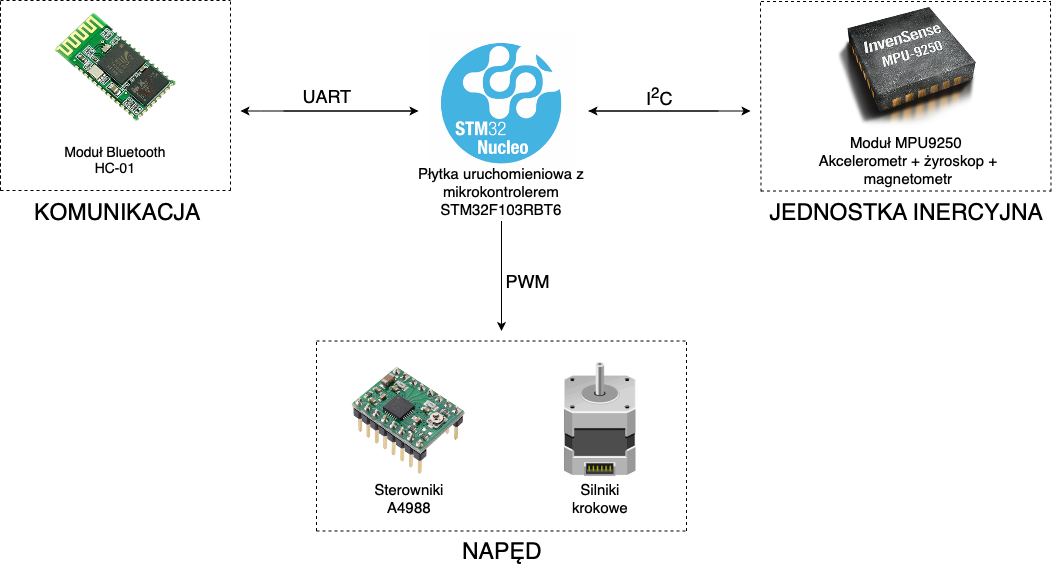
\includegraphics[width=1\textwidth]{Rysunki/Rozdzial05/Platforma_sprzetowa.png}
    \caption{Wykorzystane w budowie moduły}
    \label{Moduly}
\end{figure}

%----------------------------------------------------------------------------------------------------------------
\section{Konstrukcja mechaniczna}

Budowę robota, rozpoczęto od fazy koncepcyjnej, w której zaplanowano rozmieszczenie poszczególnych elementów, które można zobaczyć na rysunku \ref{Faza koncepcyjna}.

\begin{figure}[h!]
    \centering
    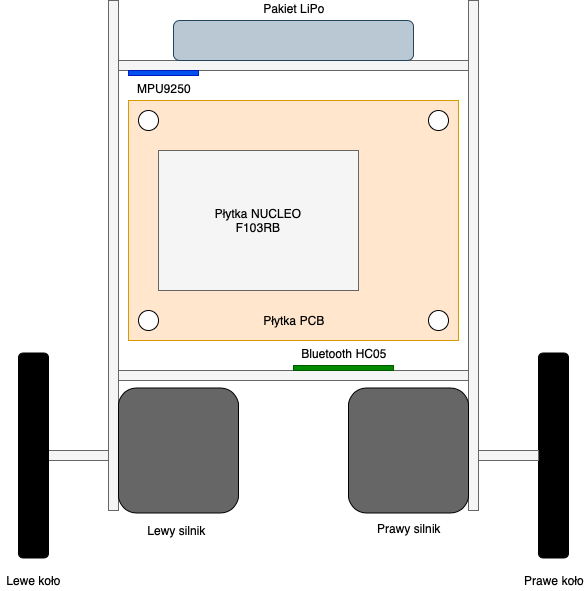
\includegraphics[width=0.5\textwidth]{Rysunki/Rozdzial05/Faza_koncepcyjna.png}
    \caption{Rozmieszczenie elementów}
    \label{Faza koncepcyjna}
\end{figure}

Kolejnym etapem, było zaprojektowanie korpusu, który zdecydowano się wykonać z poliwęglanu o grubości 5mm, ze względu na łatwą dostępność i stosunkowo niski koszt. Projekt został wykonany w programie \texttt{SolidWorks}, a rama została wykonana na zamówienie w firmie oferującej usługi laserowej obróbki poliwęglanu, na podstawie rysunków wykonawczych przedstawionych na schemacie \ref{rysunki wykonawcze}. Wyrenderowana rama robota została zaprezentowana na rysunku \ref{render}.

\begin{figure}[h!]
    \centering
    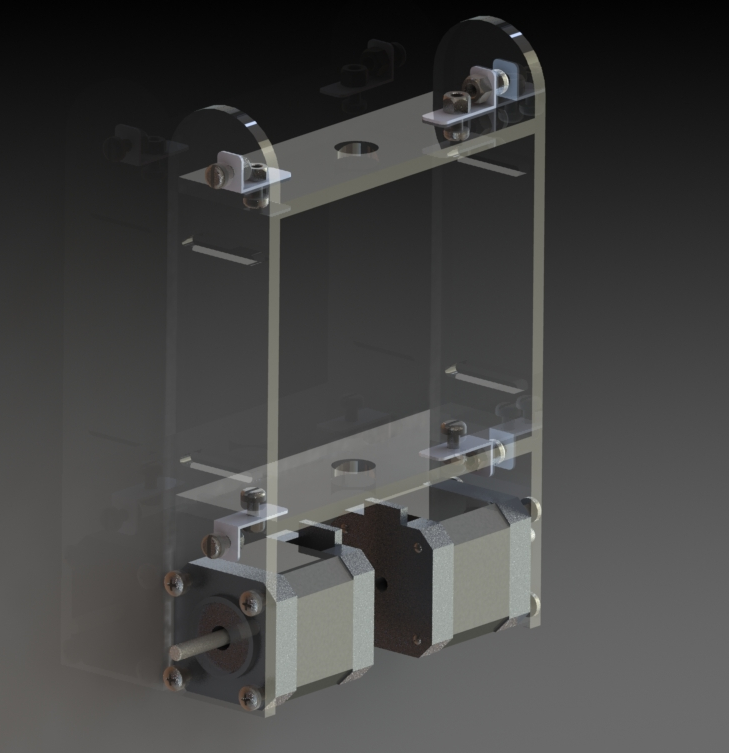
\includegraphics[width=0.5\textwidth]{Rysunki/Rozdzial05/rama.png}
    \caption{Wyrenderowany wygląd zaprojektowanego korpusu}
    \label{render}
\end{figure}

\begin{figure}[h!]
    \centering
    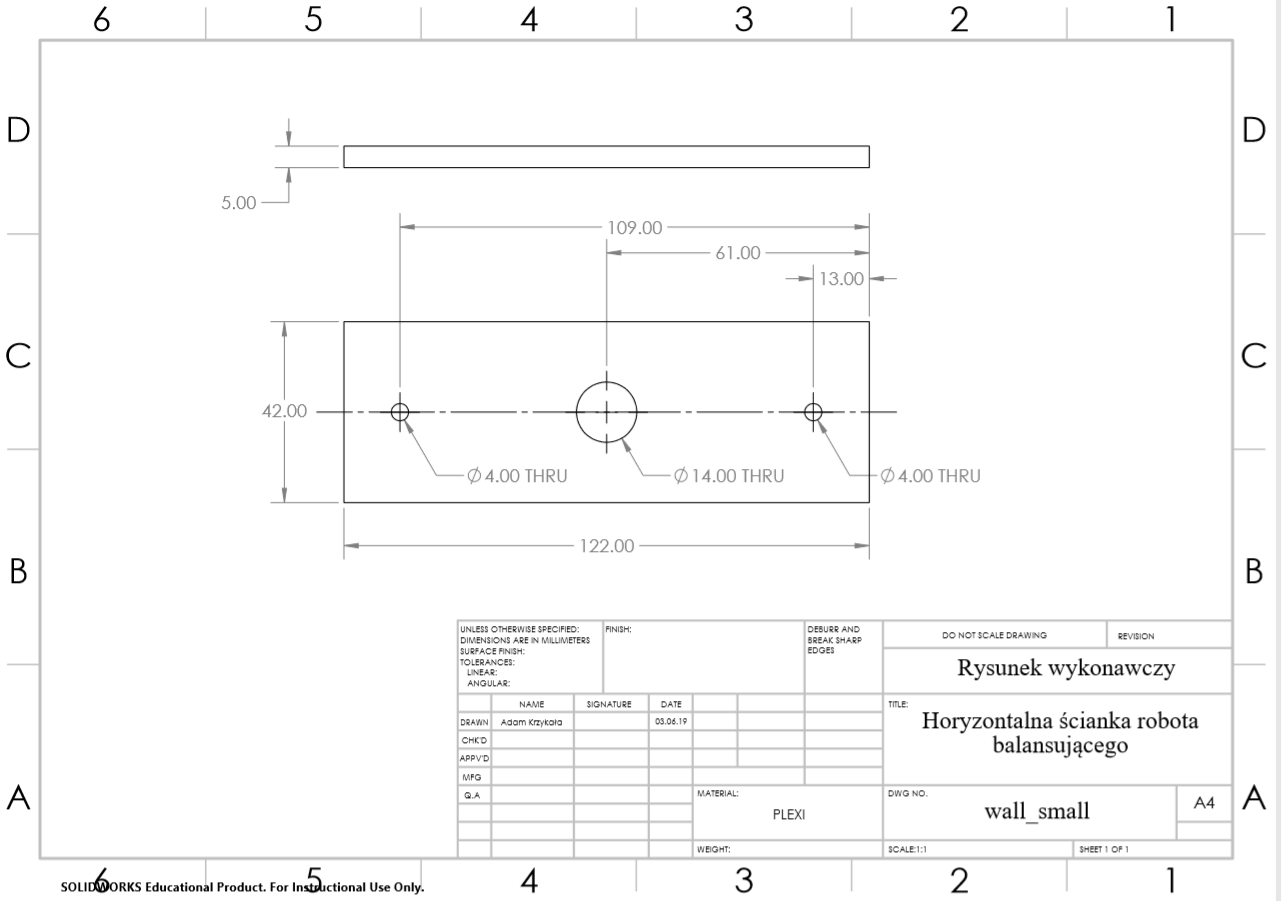
\includegraphics[width=0.5\textwidth]{Rysunki/Rozdzial05/smallWall.png}
    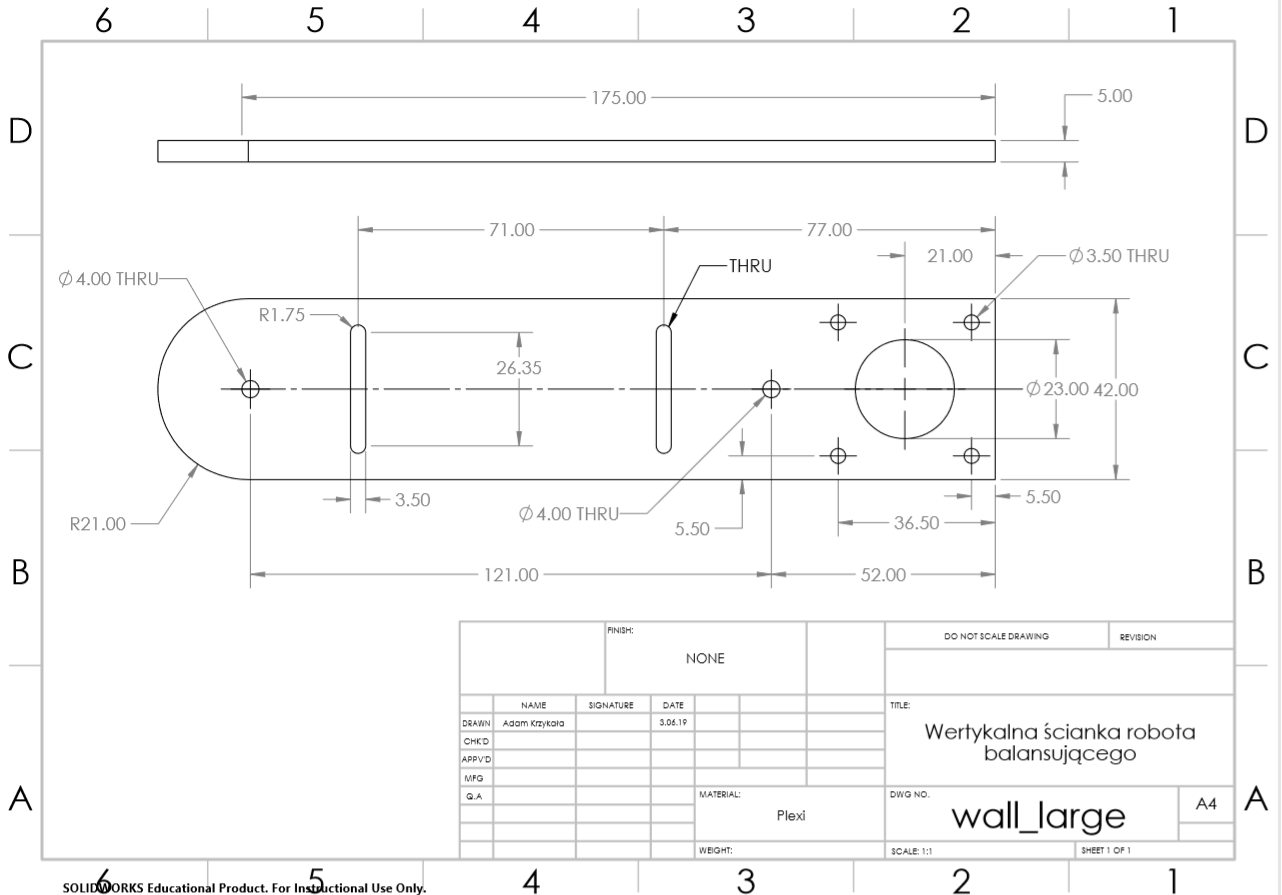
\includegraphics[width=0.5\textwidth]{Rysunki/Rozdzial05/bigWall.png}
    \caption{Rysunki wykonawcze elementów korpusu}
    \label{rysunki wykonawcze}
\end{figure}

%----------------------------------------------------------------------------------------------------------------
\section{Układ elektroniczny}

%----------------------------------------------------------------------------------------------------------------
\subsection{Zasilanie}

Silniki krokowe zasilane są bezpośrednio z pakietu LiPo. Płytka z mikrokontrolerem oraz moduł bluetooth zasilane są z przetwornicy o napięciu wyjściowym 5V. Moduł MPU9250, również jest zasilany z przetwornicy, ale o napięciu wyjściowym 3.3V. Zamiast przetwornic z powodzeniem można było użyć zwykłych stabilizatorów liniowych, jednak zdecydowano się na przetwornice ze względu na ich wbudowane zabezpieczenie nadprądowe oraz temperaturowe. Dodatkowym atutem jest możliwość wykorzystania w innych projektach, w których potrzebne jest inne napięcie wyjściowe takiej przetwornicy, ponieważ jest ono regulowane za pomocą potencjometru. Cały układ zabezpieczono dodatkowo szybkim bezpiecznikiem topikowym o maksymalnym prądzie przewodzenia 4A. Schemat układu zasilania, wraz z dzielnikiem napięcia umożliwiającym pomiar aktualnego stanu baterii za pomocą przetwornika ADC, widoczny jest na rysunku \ref{Zasilanie schemat}.

\begin{figure}[h!]
    \centering
    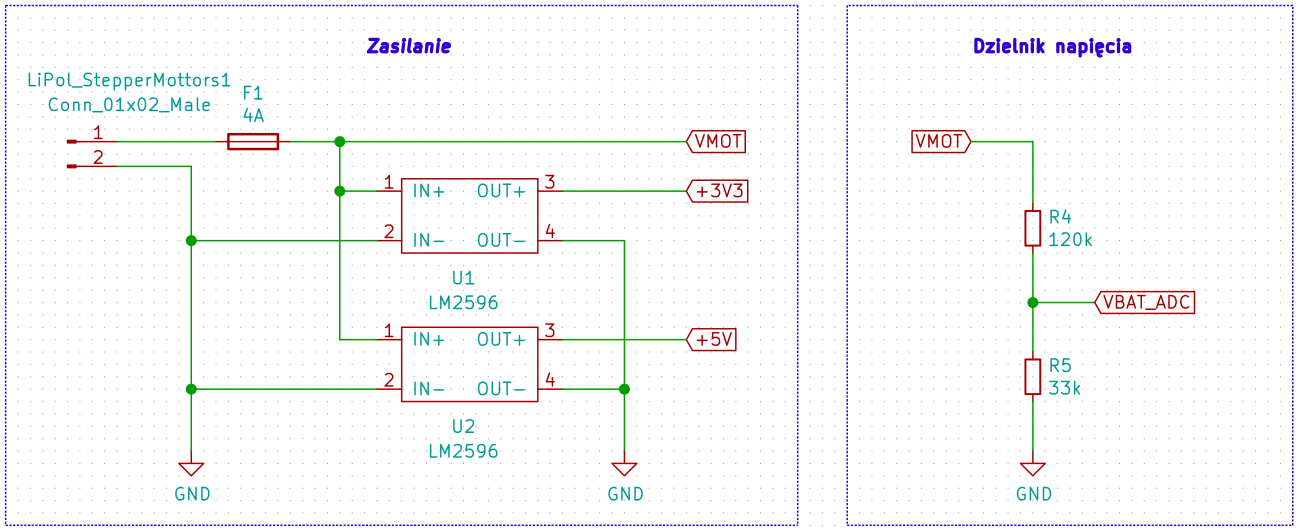
\includegraphics[width=0.75\textwidth]{Rysunki/Rozdzial05/Zasilanie_schemat.png}
    \caption{Schemat układu zasilania}
    \label{Zasilanie schemat}
\end{figure}

%----------------------------------------------------------------------------------------------------------------
\subsection{Jednostka inercyjna MPU9250}

Do zasilenia modułu MPU9250, wykorzystano napięcie 3.3V, pochodzące z przetwornicy. Do komunikacji z modułem wykorzystuje się interfejs $I^2C$. Sposób podłączenia modułu przedstawiony jest na rysunku \ref{MPU9250 schemat}. Moduł wpinany jest do płytki PCB za pomocą przewodów żeńsko-męskich oraz żeńskich goldpinów, znajdujących się na płytce.

\begin{figure}[h!]
    \centering
    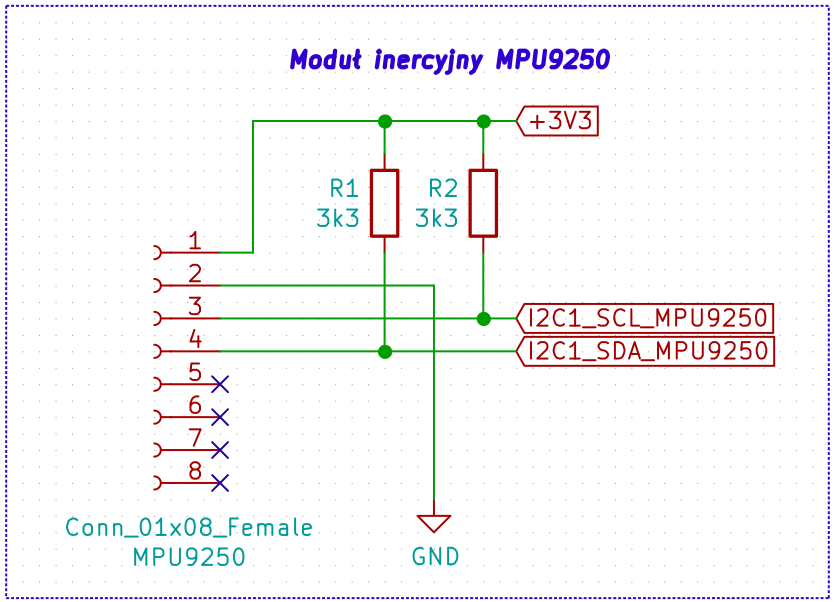
\includegraphics[width=0.5\textwidth]{Rysunki/Rozdzial05/MPU9250_schemat.png}
    \caption{Schemat układu MPU9250}
    \label{MPU9250 schemat}
\end{figure}

%----------------------------------------------------------------------------------------------------------------
\subsection{Moduł Bluetooth HC--05}

Moduł zasilić można napięciem z przedziału 3.6-6V, dlatego zdecydowano się podpiąć go do wyjścia przetwornicy o napięciu wyjściowym na poziomie 5V. Schemat podłączenia modułu przedstawia rysunek \ref{HC05 schemat}. Moduł również został wpięty do płytki PCB, za pomocą żeńskich goldpinów oraz przewodów żeńsko-męskich.

\begin{figure}[h!]
    \centering
    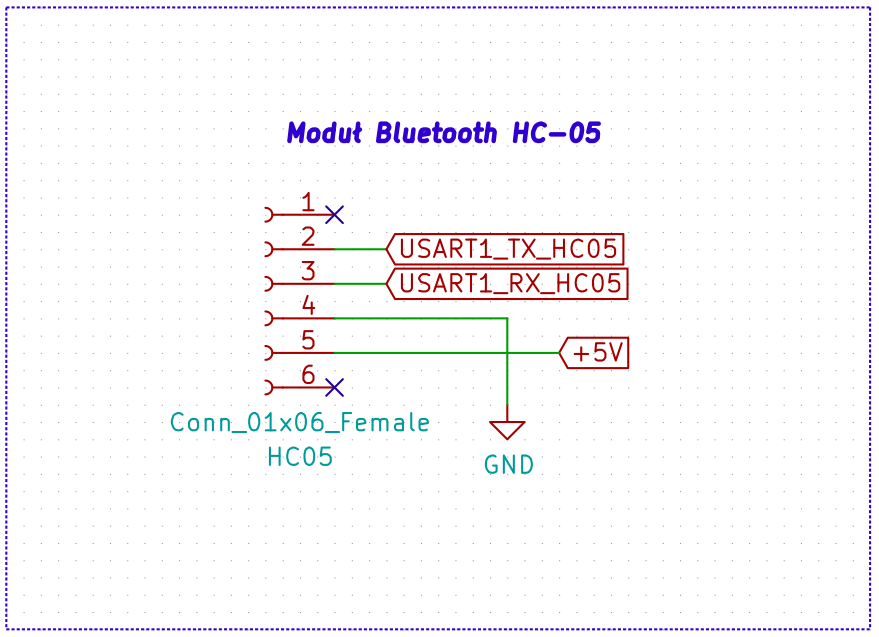
\includegraphics[width=0.5\textwidth]{Rysunki/Rozdzial05/HC05_schemat.png}
    \caption{Schemat układu HC05}
    \label{HC05 schemat}
\end{figure}

%----------------------------------------------------------------------------------------------------------------
\subsection{Silniki krokowe oraz sterowniki A4988}

Schemat połączenia sterowników przedstawia schemat \ref{A4988 schemat}. Piny MS1, MS2, MS3 zostały zmostkowane, ponieważ nie przewidywano zastosowania różnych rozdzielczości kroków dla dwóch osobnych silników. Same moduły wpięte zostały do PCB za pomocą podstawek wykonanych z żeńskich goldpinów.

\begin{figure}[h!]
    \centering
    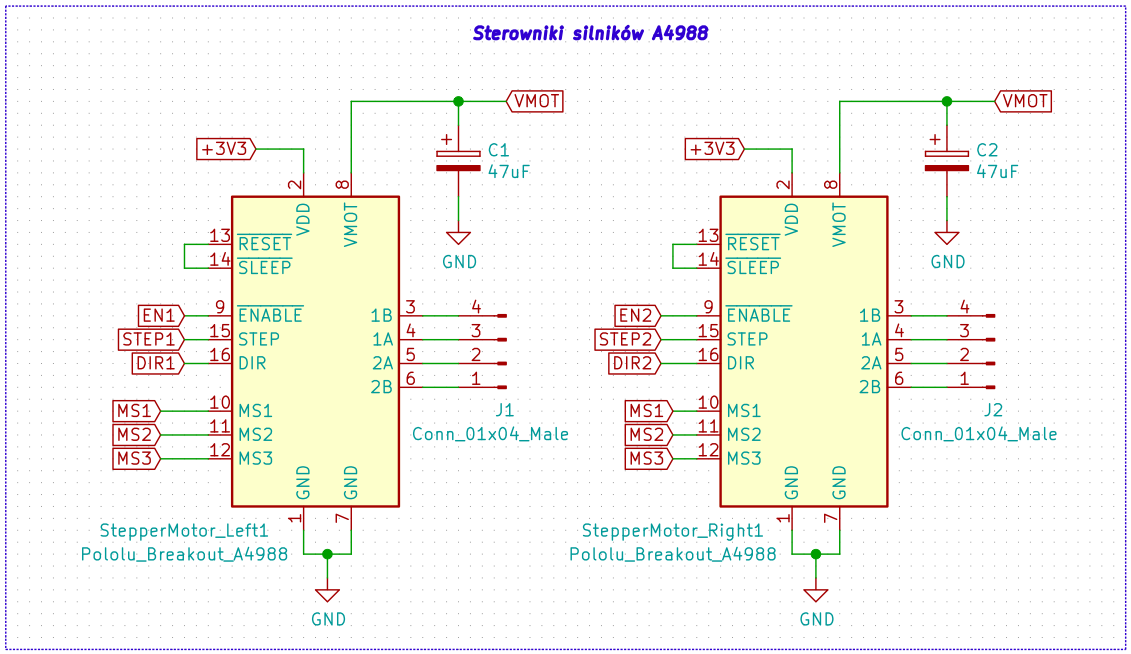
\includegraphics[width=0.75\textwidth]{Rysunki/Rozdzial05/A4988_schemat.png}
    \caption{Schemat układu A4988}
    \label{A4988 schemat}
\end{figure}

%----------------------------------------------------------------------------------------------------------------
\section{Konfiguracja mikrokontrolera i peryferiów}

Cała konfiguracja mikrokontrolera wykonana została w dedykowanym do tego programie \texttt{CubeMX w wersji 5.2.1}. Na rysunku \ref{Piny} widoczna jest konfiguracja wszystkich pinów dostępnych w mikrokontrolerze.

\begin{figure}[h!]
    \centering
    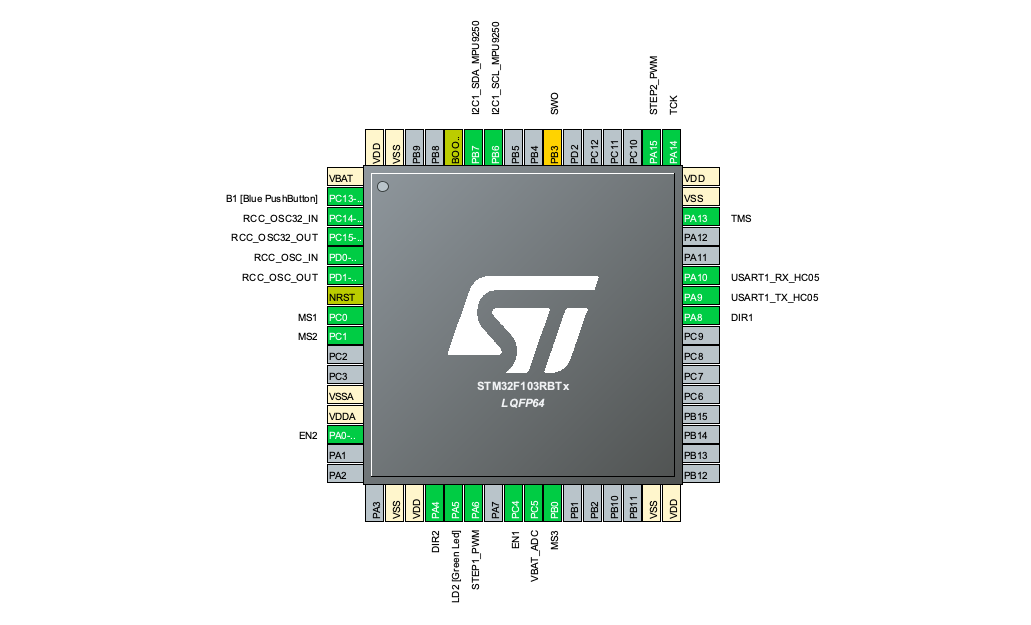
\includegraphics[width=1\textwidth]{Rysunki/Rozdzial05/Pinout.png}
    \caption{Konfiguracja pinów mikrokontrolera}
    \label{Piny}
\end{figure}

%----------------------------------------------------------------------------------------------------------------
\subsection{Zegary}

Częstotliwość taktowania głównego zegara mikrokontrolera ustawiona została na 64 MHz oraz częstotliwość magistrali timerów została ustawiona na 32 MHz. Cała konfiguracja widoczna jest na schemacie \ref{Zegary}.

\begin{figure}[h!]
    \centering
    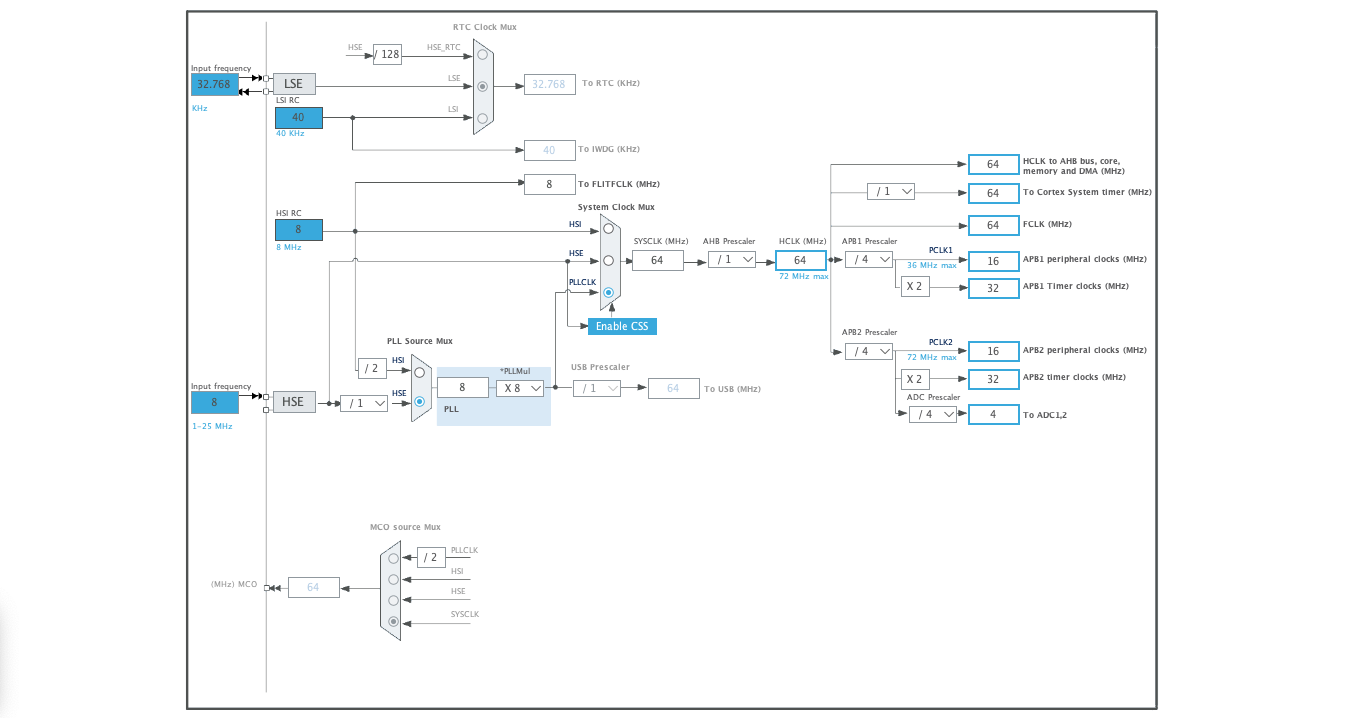
\includegraphics[width=1\textwidth]{Rysunki/Rozdzial05/Zegary.png}
    \caption{Konfiguracja zegarów mikrokontrolera}
    \label{Zegary}
\end{figure}

%----------------------------------------------------------------------------------------------------------------
\subsection{ADC}

Najważniejsze parametry ustawione dla przetwornika ADC, to pomiar na kanale 15 powiązanym z pinem PC5, do którego podpięto wyjście dzielnika napięcia dla zasilania oraz zwiększenie liczby cykli do 239.5, w trakcie których następuje pomiar. Większa ilość cykli zwiększa dokładność pomiaru. Inne parametry konfiguracyjne znajdują się w tabeli \ref{Konfiguracja przetwornika ADC}.

\begin{table}[h!]
    \centering
    \caption{Konfiguracja przetwornika ADC}
    \begin{tabular}{|c|c|}
        \hline
        Mode & Independent mode \\
        \hline
        Data Alignment & Right alignment \\
        \hline
        Scan Conversion Mode & Disabled \\
        \hline
        Continuous Conversion Mode & Disabled \\
        \hline
        Discontinuous Conversion Mode & Disabled \\
        \hline
        Enable Regular Conversions & Enable \\
        \hline
        Number Of Conversion &  1 \\
        \hline
        External Trigger Conversion Source & Regular Conversion launched by software \\
        \hline
        Rank & 1 \\
        \hline
        Channel & Channel 15 \\
        \hline
        Sampling Time & 239.5 Cycles \\
        \hline
    \end{tabular}
    \label{Konfiguracja przetwornika ADC}
\end{table}

%----------------------------------------------------------------------------------------------------------------
\subsection{PWM}

Jeśli chodzi o generator sygnałów PWM, to są nim dwa osobne timery. Pierwszy z nich z wyjściem na pinie PA6, a drugi z wyjściem na pinie PA15. Preskaler został domyślnie ustawiony na 0, ponieważ i tak jest modyfikowany w trakcie działania programu w celu zmiany częstotliwości generowanego sygnału. Wartość ARR - 1 (Counter Period), mówi o ilości dostępnych poziomów wypełnienia sygnału. W tym przypadku dostępne jest 1000 poziomów wypełnienia, czyli 0.1\%, 0.2\%, ... , 100\%. 

\begin{table}[h!]
    \centering
    \caption{Konfiguracja timerów generujących sygnał PWM}
    \begin{tabular}{|c|c|}
        \hline
        Prescaler (PSC 16 bits value) & 0 \\
        \hline
        Counter Mode & Up \\
        \hline
        Counter Period (Auto Reload Register - 16 bits value ) & 999 \\
        \hline
        Internal Clock Division (CKD) & No Division \\
        \hline
        auto\-reload preload & disable \\
        \hline
        Master/Slave Mode (MSM bit) & Disable (Trigger input effect not delayed) \\
        \hline
        Trigger Event Selection & Reset (UG bit from TIMx EGR) \\
        \hline
        Mode & PWM mode 1 \\
        \hline
        Pulse (16 bits value) & 0 \\
        \hline
        Fast Mode & Disable \\
        \hline
        CH Polarity & High \\
        \hline
    \end{tabular}
    \label{Konfiguracja PWM}
\end{table}

%----------------------------------------------------------------------------------------------------------------
\subsection{$\mathbf{I^{2}C}$}

Interfejs komunikacyjny $I^2C$ służący do obsługi modułu MPU9250, posiada ustawienia domyślne przedstawione w tabeli \ref{Konfiguracja portu I2C}.

\begin{table}[h!]
    \centering
    \caption{Konfiguracja portu $I^2C$}
    \begin{tabular}{|c|c|}
        \hline
        I2C Speed Mode & Standard Mode \\
        \hline
        I2C Clock Speed (Hz) & 100000 \\
        \hline
        Clock No Stretch Mode & Disabled \\
        \hline
        Primary Address Length selection & 7-bit \\
        \hline
        Dual Address Acknowledged & Disabled \\
        \hline
        Primary slave address & 0 \\
        \hline
        General Call address detection & Disabled \\
        \hline
    \end{tabular}
    \label{Konfiguracja portu I2C}
\end{table}

%----------------------------------------------------------------------------------------------------------------
\subsection{USART}

Prędkość transmisji interfejsu komunikacyjnego USART ustawiona została na 115200 bodów/s ze względu na stosunkowo duży rozmiar wysyłanej do komputera ramki danych. Reszta ustawień pozostała domyślna i zaprezentowana jest w tabeli \ref{Konfiguracja USART}.

\begin{table}[h!]
    \centering
    \caption{Konfiguracja portu USART}
    \begin{tabular}{|c|c|}
        \hline
        Baud Rate & 115200 \\
        \hline
        Word Length & 8 Bits (including Parity) \\
        \hline
        Parity & None \\
        \hline
        Stop Bits & 1 \\
        \hline
        Data Direction & Receive and Transmit \\
        \hline
        Over Sampling & 16 Samples \\
        \hline
    \end{tabular}
    \label{Konfiguracja USART}
\end{table}

%----------------------------------------------------------------------------------------------------------------
\section{Oprogramowanie}

Oprogramowanie na mikrokontroler napisane zostało w oparciu o darmową dystrybucję systemu czasu rzeczywistego \texttt{FreeRTOS}. Zaimplementowano pięć wątków, których idea zastosowania została przedstawiona na rysunku \ref{Watki}. 

\begin{figure}[h!]
    \centering
    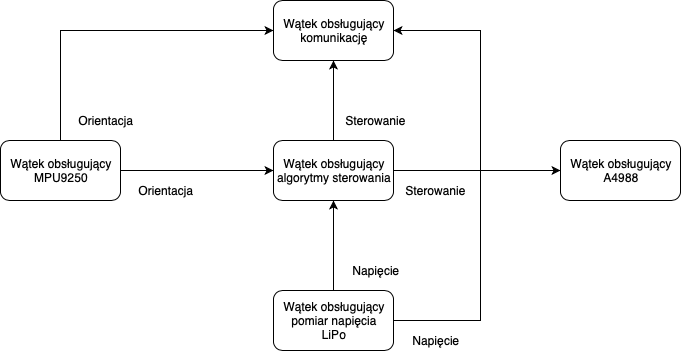
\includegraphics[width=0.75\textwidth]{Rysunki/Rozdzial05/Software.png}
    \caption{Struktura podziału programu na wątki}
    \label{Watki}
\end{figure}

%----------------------------------------------------------------------------------------------------------------
\subsection{Pomiar stanu naładowania baterii}

W projekcie do zasilania wykorzystano baterię LiPo 3S 1300mAh, o nominalnym napięciu pracy 11.1V, czyli 3.7V dla każdej z pojedynczych cel. Dla w pełni naładowanej baterii, jej napięcie wynosi 12.6V, czyli 4.2V dla pojedynczej celi. Napięcie podczas użytkowania nie powinno wynieść mniej niż 2.7V, dla pojedynczej celi, a 8.1V dla całego pakietu. Jest to napięcie graniczne i grozi uszkodzeniem baterii.

W projekcie zdecydowano się na programowe zabezpieczenie przed nadmiernym rozładowaniem. Z racji tego, że pomiar napięcia wykonywany jest dla całej baterii jednocześnie, a nie dla każdej celi osobno zdecydowano się zawyżyć graniczne napięcie zasilania z 8.1V do 10.5V, poniżej którego następuje cykliczne zapalanie i gaszenie diody LD2 umieszczonej na płytce, która pełni rolę komunikatu ostrzegawczego. Poniżej 10V, następuje odcięcie zasilania silników krokowych.

Tak, aby nie uszkodzić przetwornika ADC, dla którego napięcie wejściowe nie może przekroczyć jego napięcia zasilania, zostało ono obniżone do 2.72V dla maksymalnego naładowania baterii, za pomocą dzielnika napięcia, którego stosunek napięcia wejściowego do wyjściowego wynosi $\frac{12.6}{2.72} \approx 4.632$

Pomiar pochodzący z przetwornika ADC, przeliczany jest na napięcie wyrażone w woltach w następujący sposób
$$
    \frac{3.3 \cdot \textrm{Odczyt ADC}}{4096 - 1} \cdot 4.632
$$
gdzie liczba 4096 oznacza rozdzielczość przetwornika, a 3.3 napięcie zasilania przetwornika.

Jako pomiar uznaje się średnią ze 100 pomiarów, w celu uniknięcia odchyłek odczytów w krótkich odstępach czasu, wynikających z niedokładności pomiaru.

%----------------------------------------------------------------------------------------------------------------
\subsection{Algorytm sterowania}

Obsługa algorytmu sterowania odbywa się w wątku \texttt{Control\_Task}, wewnątrz którego zaimplementowana została kaskada dwóch regulatorów PID, którą zaprezentowano w rozdziale \ref{chap:analizaruchurobota}, w części dotyczącej sterowania. Różnica pomiędzy symulacją, a implementacją algorytmu sterowania na mikrokontrolerze polega na wprowadzeniu możliwości skręcania prawo--lewo, a nie jazdy tylko przód--tył. Dlatego każde koło posiada swoją niezależnie działającą kaskadę regulatorów PID, tak aby możliwe było zadawanie różnych prędkości dla dwóch kół, co zostało przedstawione na schemacie \ref{Algorytm}.

\begin{figure}[h!]
    \centering
    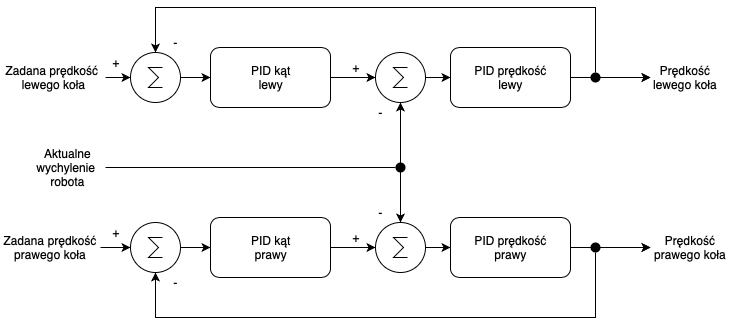
\includegraphics[width=0.75\textwidth]{Rysunki/Rozdzial05/Algorytm_sterowania.png}
    \caption{Algorytm sterowania oparty na kaskadzie regulatorów PID}
    \label{Algorytm}
\end{figure}

Układ regulacji nie uwzględnia kierunku obrotu silników, dlatego wykorzystując prędkości na wyjściu regulatora należy wziąć je z przeciwnymi znakami, tak aby silniki kręciły się w tym samym kierunku.

%----------------------------------------------------------------------------------------------------------------
\subsection{Obsługa czujnika ruchu}

Obsługa czujnika MPU9250 odbywa się w wątku \texttt{IMU\_Task}, który co 5ms odczytuje pomiary z rejestrów czujnika, a następnie wykorzystując jeden z trzech zaimplementowanych metod fuzji sygnałów przelicza je na wartości kąta Roll, Pitch i Yaw. W algorytmie sterowania wykorzystywany jest kąt Pitch, ponieważ osią równoległą do osi obrotu wahadła jest oś Y. 

Zakres pracy poszczególnych czujników jaki został ustawiony oraz współczynnik służący do przeliczenia odczytów z rejestrów dotyczących pomiarów zaprezentowane są w tabeli \ref{zakresy}.

\begin{table}[h!]
    \centering
    \caption{Zakresy pracy dla czujników}
    \begin{tabular}{|c|c|c|}
        \hline
        Czujnik & Zakres pracy & Współczynnik \\
        \hline
        Żyroskop & $+/- 2000 ^o/s$ & 16.4 \\
        \hline
        Akcelerometr & $+/- 2g$ & 16.384 \\
        \hline
        Magnetometr & $+/- 48\mu T$ & 0.6 \\
        \hline
    \end{tabular}
    \label{zakresy}
\end{table}

Dzięki temu po odczytaniu z odpowiednich rejestrów wartości pomiarów możemy przeliczyć je na interesujące nas wielkości fizyczne w następujący sposób
$$
    \textrm{Prędkość kątowa} = \frac{LSB}{16.4}
$$
$$
    \textrm{Przyspieszenie liniowe} = \frac{LSB}{16.384}
$$
$$
    \textrm{Natężenie pola magnetycznego} = \frac{LSB}{0.6}
$$
gdzie LSB - oznacza pomiar odczytany z rejestru dla danego czujnika i danej osi.

W przypadku magnetometru konieczne jest jeszcze uwzględnienie czułości pomiaru dla każdej osi odczytywane z rejestrów ASAX, ASAY,ASAZ, dlatego ostateczna postać wartości natężenia pola magnetycznego wynosi
$$
    \textrm{Natężenie pola magnetycznego} = \frac{LSB}{0.6} \cdot \left(\frac{(ASA-128)\cdot 0.5}{128}-1\right)
$$
gdzie \\
LSB -- pomiar dla danej osi \\
ASA -- współczynnik czułości dla danej osi

Podczas implementacji obsługi czujnika bardzo ważną rzeczą i należy uwzględnić to w obliczeniach jest inna orientacja osi akcelerometru i żyroskopu względem osi magnetometru, co przedstawione zostało na rysunku \ref{Orientacja}

\begin{figure}[h!]
    \centering
    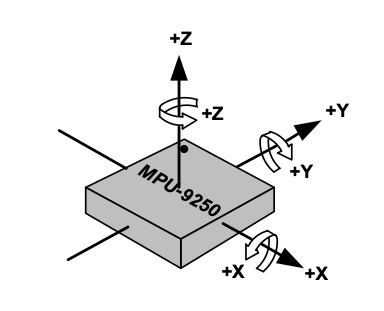
\includegraphics[width=0.35\textwidth]{Rysunki/Rozdzial05/AcceGyro_osie.png}
    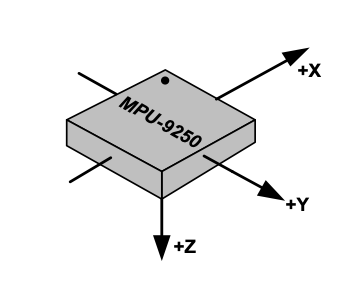
\includegraphics[width=0.35\textwidth]{Rysunki/Rozdzial05/Mag_osie.png}
    \caption{Orientacja osi akcelerometru i żyroskopu po lewej oraz magnetometru po prawej }
    \label{Orientacja}
\end{figure}

Więcej informacji o tym jak skonfigurować moduł, jakie inne funkcje posiada oraz mapę rejestrów, wraz ze szczegółowym opisem znajdziemy w jego dokumentacji technicznej \cite{MPU9250datascheet}, oraz mapie rejestrów \cite{MPU9250registermap}. 

\newpage
%----------------------------------------------------------------------------------------------------------------
\subsection{Obsługa silników krokowych}

Do sterowania silnikami krokowymi, wykorzystano sterowniki A4988, za których obsługę odpowiedzialny jest wątek \texttt{Engines\_Task}. Do głównych zadań wątku należy wysterowanie prędkości obrotowej silników krokowych na podstawie zadanych prędkości silników oraz odcięcie zasilania silników w momencie wciśnięcia przycisku awaryjnego lub zejścia napięcia baterii zasilającej poniżej założonej bezpiecznej granicy.

Za pomocą sterownika i jego pinów MS1,MS2,MS3 ustawiamy rozdzielczość silników na wartość 1/8 kroku podając na piny MS1 i MS2 wysoki stan logiczny, a na piny MS3 niski stan logiczny. Za pomocą pinu EN, możemy załączać lub wyłączań zasilanie na uzwojeniach silników. Wybranie odpowiedniego stanu logicznego na pinie DIR, decyduje o kierunku obrotu wału silnika, natomiast każdorazowa zmiana stanu logicznego na pinie STEP, powoduje wykonanie pojedynczego kroku przez silnik, dlatego zdecydowano się podłączyć do tego pinu sygnał PWM.

Sygnał PWM generowany jest przez timer, dlatego zmieniając wartość preskalera możemy decydować o częstotliwości zmiany stanu generowanego sygnału, a co za tym idzie ilością generowanych kroków w danym okresie czasu, z którego możemy obliczyć prędkość silnika wyrażoną w obrotach na minutę (RPM). Wartość wypełnienia sygnału jest stała i wynosi 50\%. 

Chcąc wyznaczyć wartość preskalera, w celu zadawania prędkości obrotowej silnika, musimy znać wartość odstępów między poszczególnymi krokami. Wyznacza się go korzystając z wartości kąta jaki zakreśla wał silnika podczas wykonywania kroku (w silnikach zastosowanych w projekcie jest to $1.8^o$ dla pełnego kroku).

Po kolei obliczamy wartość kąta na krok dla ustawionej rozdzielczości kroku
$$
    \frac{1.8^o}{8} = 0.225^o
$$
ilość kroków na pełny obrót
$$
    \frac{360^o}{0.225^o} = 1600
$$
ilość kroków na minutę dla zadanej przez nas prędkości np. 100 RPM
$$
    100 \cdot 1600 = 160000
$$
oraz wartość odstępu pomiędzy krokami w ciągu minuty (60000000 ms)
$$
    \frac{60000000ms}{160000} = 375 ms
$$
Wartość preskalera dla zadanej prędkości obrotowej 100RPM, częstotliwości taktowania timera 32MHz oraz wartości rejestru ARR równej 999 wynosi
$$
    PSC = \frac{32MHz * 375ms}{ARR + 1} - 1 = 23
$$
Wartość preskalera obliczamy analogicznie do innych wartości zadanej prędkości obrotwej.

%----------------------------------------------------------------------------------------------------------------
\subsection{Komunikacja bezprzewodowa z komputerem}

Do bezprzewodowej komunikacji robota z komputerem wykorzystano gotowy moduł bluetooth HC-05. Aby programować moduł w trybie komend AT, należy podłączyć moduł z komputerem za pomocą konwertera UART--USB, prędkość transmisji ustawić na 38400 bodów oraz wysłać komendę AT za pomocą dowolnego terminala. Jeśli moduł odpowie OK, możemy rozpocząć zmianę jego ustawień. Podczas konfiguracji, dokonano następujących zmian
\begin{itemize}
    \item nazwy wyświetlanej podczas wyszukiwania modułu -- AT+NAME = "BRobot"
    \item hasła dostępu do modułu -- AT+PSWD = "****"
    \item parametrów transmisji -- AT+UART = "115200,1,0" (baud 115200, 1 bit stopu, brak kontroli parzystości)
\end{itemize}

Za komunikację z komputerem odpowiedzialny jest wątek o nazwie \texttt{USART\_Task}, którego głównym zadaniem jest cykliczne parsowanie i wysyłanie informacji do komputera co 10ms. Wysyłane dane parsowane są do ramki w postaci

\begin{table}[h!]
    \centering
    \caption{Wysyłana do komputera ramka danych}
    \begin{tabular}{|c|c|}
        \hline
        int16\_t & Napięcie baterii \\
        \hline
        3 x int16\_t & Kąt Roll,Pitch, Yaw na wyjściu filtra \\
        \hline
        2 x int16\_t & Prędkość lewego i prawego silnika \\
        \hline
        3 x int16\_t & Odczyty z żyroskopu w osi X,Y,Z \\
        \hline
        3 x int16\_t & Odczyty z akcelerometru w osi X,Y,Z \\
        \hline
        3 x int16\_t & Odczyty z magnetometru w osi X,Y,Z \\
        \hline
        int8\_t & CRC \\
        \hline
    \end{tabular}
    \label{Ramka wysylana}
\end{table}
gdzie CRC jest cyklicznym kodem nadmiarowym służącym do kontroli poprawności odebranej ramki po stronie komputera.

Parsowanie danych z komputera odbywa się w obsłudze przerwania, wywoływanego przez interfejs UART w momencie odebrania danych. Odebrane dane są ramką w postaci

\begin{table}[h!]
    \centering
    \caption{Odbierana z komputera ramka danych}
    \begin{tabular}{|c|c|}
        \hline
        3 x int16\_t & Nastawy regulatora PID dla kąta wychylenia \\
        \hline
        3 x int16\_t & Nastawy regulatora PID dla prędkości silników \\
        \hline
        int16\_t & Parametr $\alpha$ dla filtru komplementarnego \\
        \hline
        int16\_t & Parametr $r$ dla filtru Kalmana \\
        \hline
        int8\_t & Wartość 0,1. Jeśli 1 to stop awaryjny jest wciśnięty \\
        \hline
        int8\_t & Wartość 0,1,2 decydująca o tym, który filtr jest włączony \\
        \hline
        int8\_t & CRC \\
        \hline
    \end{tabular}
    \label{Ramka wysylana}
\end{table}

%----------------------------------------------------------------------------------------------------------------
\subsection{Fotografie}

\textcolor{red}{DOŁĄCZYĆ FOTOGRAFIE ROBOTA}
%----------------------------------------------------------------------------------------------------------------
\chapter{Aplikacja do wizualizacji danych sensorycznych i komunikacji z robotem}
\label{chap:aplikacja}

W celu ułatwienia procesu strojenia filtrów oraz regulatorów PID stworzono aplikację, którą wyposażono dodatkowo w graficzną reprezentację danych pochodzących z robota w postaci wykresów i wizualizacji 3D. Pozwoliło to wyeliminować problem polegający na konieczności wgrywania za każdym razem nowego programu do mikrokontrolera sterującego robotem w celu zmiany któregokolwiek z parametrów oraz pozwoliło wykryć błędy na etapie implementacji fuzji sygnałów.

%----------------------------------------------------------------------------------------------------------------
\section{Struktura programu}

Główna część programu składa się z zaimplementowanych trzech klas
\begin{itemize}
    \item \texttt{Bluetooth} -- odpowiedzialnej za warstwę komunikacyjną opartą na \texttt{QSerialPort}
    \item \texttt{CommunicationWindow} -- odpowiedzialnej za obsługę interfejsu graficznego okna służącego do nawiązania połączenia z robotem
    \item \texttt{MainWindow} -- odpowiedzialnej za obsługę interfejsu graficznego głównego okna aplikacji
\end{itemize}

Wszystkie wymienione powyżej klasy komunikują się za pomocą mechanizmu slotów i sygnałów, np. klasa \texttt{Bluetooth} po odebraniu i sparsowaniu danych z robota, nadaje sygnał \texttt{Parsed\_frame\_OK()}, który jest powiązany z metodą \texttt{RealTime\_data\_SLOT()} klasy \texttt{MainWindow}, wewnątrz której następuje wyrysowanie danych w oknie głównym aplikacji. 
%----------------------------------------------------------------------------------------------------------------
\section{Funkcjonalności programu}

%----------------------------------------------------------------------------------------------------------------
\subsection{Transmisja dwukierunkowa z robotem}

Za obsługę transmisji odpowiedzialna jest wbudowana w środowisko \texttt{Qt} klasa \texttt{QSerialPort}. Posiada ona szereg metod ułatwiających współpracę z portami dostępnymi na komputerze. Między innymi za pomocą takich metod jak
\begin{itemize}
    \item \texttt{bool setParity(QSerialPort::Parity parity)}
    \item \texttt{bool setBaudRate(qint32 baudRate, QSerialPort::Directions directions = AllDirections)}
    \item \texttt{bool setStopBits(QSerialPort::StopBits stopBits)}
    \item \texttt{bool setDataBits(QSerialPort::DataBits dataBits)}
\end{itemize}
służących do ustawiania parametrów transmisji, oraz
\begin{itemize}
    \item \texttt{virtual void close() override}
    \item \texttt{virtual bool open(QIODevice::OpenMode mode) override}
    \item \texttt{virtual qint64 readData(char *data, qint64 maxSize) override}
    \item \texttt{virtual qint64 writeData(const char *data, qint64 maxSize) override}
\end{itemize}
za pomocą, których zaimplementowano transmisję dwukierunkową z robotem.

Odbieranie i przetwarzanie danych odbywa się na zasadzie przerwania, którego obsługa wykonywana jest po wykryciu sygnału \texttt{readyRead()} generowanego przez obiekt klasy \texttt{QSerialPort} po odebraniu całej ramki danych. Odebrane dane są odpowiednio parsowane i wyświetlane w odpowiednich miejscach.

%----------------------------------------------------------------------------------------------------------------
\subsection{Wyświetlanie danych dotyczących czujnika ruchu i fuzji sygnałów}

Do rysowania wykresów w czasie rzeczywistym, wykorzystano zewnętrzną bibliotekę \texttt{QCustomPlot}. Do funkcji wbudowanych w bibliotekę, które ułatwiają obsługę wykresów należą
\begin{itemize}
    \item zmiana rozdzielczości osi czasu
    \item zmiana zakresów osi X i Y
    \item zmiana kolorów wyświetlanych wykresów
    \item automatycznie skalowanie się zakresu osi w zależności od wyświetlanych danych
\end{itemize}

%----------------------------------------------------------------------------------------------------------------
\subsection{Sterowanie jazdą robota}

Sterowanie jazdą robota, odbywa się za pomocą strzałek wyrysowanych w głównym oknie aplikacji. Po naciśnięciu odpowiedniej strzałki za pomocą myszy, zmienia ona swój kolor na zielony, w celu zasygnalizowania aktualnie zadanego kierunku ruchu. Po naciśnięciu przycisku awaryjnego zmienia on swój stan na wciśnięty i aby go odblokować należy wcisnąć go ponownie. Zmiana prędkości zadanej odbywa się za pomocą suwaka i wyrażona jest w jednostce RPM.          

%----------------------------------------------------------------------------------------------------------------
\section{Interfejs graficzny}

Cały interfejs graficzny został podzielony na dwa główne okna. Pierwsze z nich to okno służące do konfiguracji i połączenia się z portem szeregowym, oraz główne okno, w którym dostępna jest całą reszta funkcjonalności aplikacji. 

%----------------------------------------------------------------------------------------------------------------
\subsection{Okno łączenia}

Okno podzielone jest na trzy główne obszary, których rozmieszczenie zaprezentowano na rysunku \ref{Okno laczenie koncepcja}.
W pierwszym obszarze okna oznaczonym numerem 1 na rysunku \ref{Okno laczenie koncepcja}, znajdują się rozwijane opcje dotyczące portu szeregowego, z którego odczytywane są dane pochodzące z robota w postaci bitowej ramki danych. Do stworzenia rozwijanych list wykorzystano klasę \texttt{QComboBox}.

W obszarze drugim użytkownik aplikacji ma do dyspozycji trzy przyciski:
\begin{itemize}
    \item Szukaj urządzeń -- po naciśnięciu przycisku wyszukiwane są wszystkie porty, a następnie dodawane są do rozwijanej listy
    \item Połącz -- łączy się z portem, który aktualnie został wybrany z rozwijanej listy
    \item Rozłącz -- rozłącza się z aktualnie połączonym portem
\end{itemize}

Obszar trzeci jest konsolą służącą do wyświetlania komunikatów dla użytkownika. Jest to obiekt stworzony za pomocą klasy \texttt{QTextBrowser}. Ponadto w oknie dostępne są dwa przyciski: ,,Anuluj'' oraz ,,Dalej''. Pierwszy z nich kończy działanie aplikacji, natomiast drugi, po poprawnym nawiązaniu połączenia otwiera główne okno aplikacji. Rzeczywisty wygląd okna łączenia z robotem, widoczny jest na zrzucie ekranu \ref{Okno laczenie}.

\begin{figure}[h!]
    \centering
    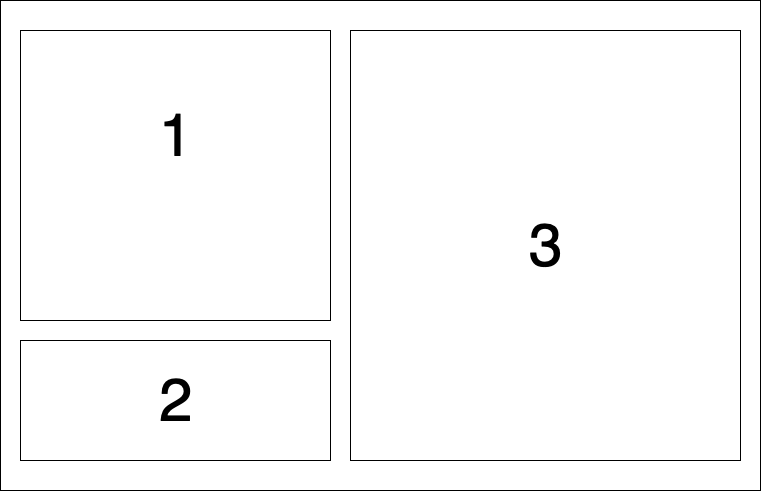
\includegraphics[width=0.75\textwidth]{Rysunki/Rozdzial06/Laczenie_okno_koncepcja.png}
    \caption{Rozmieszczenie elementów w oknie do łączenia z robotem}
    \label{Okno laczenie koncepcja}
\end{figure}

%----------------------------------------------------------------------------------------------------------------
\subsection{Główne okno}

Mając przed oczami główne okno aplikacji w jej lewym górnym rogu oznaczonym jako obszar pierwszy, wyświetla się nazwa aktualnie otwartego portu szeregowego. W prawym, górnym rogu, w obszarze numer dwa dotyczącym zasilania robota, znajduje się aktualne napięcie baterii oraz procentowe określenie stanu naładowania. W zależności od poziomu naładowania wyświetlane są trzy stany naładowania w postaci ikon o kolorze czerwonym (0-24\%), pomarańczowym (25-74\%) oraz zielonym (75-100\%). Do wyświetlania statycznych obiektów graficznych w formacie PNG, wykorzystano klasę \texttt{QPixMap} oraz \texttt{QLabel}.

W trzecim obszarze znajduje się obiekt graficzny stworzony z wykorzystaniem klasy \texttt{QTabWidget}. Za jego pomocą możemy definiować zakładki, z których każda jest oddzielnym oknem, w którym możemy umieszczać inne obiekty graficzne. Na potrzeby aplikacji stworzono pięć zakładek:
\begin{itemize}
    \item Żyroskop -- wykres z aktualnymi odczytami dla żyroskopu w osiach XYZ wyrażonymi w $^o/s$
    \item Akcelerometr -- wykres z aktualnymi odczytami dla akcelerometru w osiach XYZ wyrażonymi w $g$
    \item Magnetometr -- wykres z aktualnymi odczytami dla magnetometru w osiach XYZ wyrażonymi w $\mu T$
    \item Fuzja pomiarów -- wykres z aktualnymi wartościami obliczonymi przez aktualnie wybrany algorytm fuzji sygnałów wyrażonymi w kątach RPY
    \item Panel sterowania -- aktualne nastawy regulatorów PID oraz możliwość ich edycji, podgląd zmiennych odbieranych z robota, możliwość zmiany parametrów związanych z algorytmami fuzji sygnałów, wybranie filtru aktualnie biorącego udział w algorytmie sterowania
\end{itemize}

W obszarze numer cztery, użytkownik ma podgląd na aktualną orientację robota wyświetlaną w środowisku \texttt{OpenGL}, na podstawie odebranych kątów RPY obliczonych przez mikrokontroler robota. Zaraz poniżej w obszarze numer pięć użytkownik ma dostęp do panelu sterowania za pomocą, którego możliwe jest wymuszenie poruszania się robota w przód-tył oraz prawo-lewo, za pomocą czterech strzałek. Dodatkowo stworzono przycisk awaryjny, który po naciśnięciu przesyła do robota informację o tym, aby wyłączył napęd. Tak, aby możliwe było zmienianie aktualnej prędkości zadanej robota, wykorzystano do tego suwak stworzony za pomocą klasy \texttt{QSlider}, oraz podgląd za pomocą klasy \texttt{QLCDNumber}. Rzeczywisty wygląd okna zobaczyć, można na zrzutach ekranu, \ref{Okno panel}, \ref{Okno fuzja}, \ref{Okno zyro}.

Na samym dole okna zdefiniowano przyciski z następującymi funkcjami:
\begin{itemize}
    \item Stop -- zatrzymuje rysowanie wykresu
    \item Resetuj -- czyści wykres
    \item Wyśrodkuj -- maksymalizuje okno aplikacji po ręcznej zmianie jego wymiarów za pomocą myszki
    \item Rozłącz -- rozłącza aktualny port i przechodzi do okna łączenia
    \item Wyślij -- wysyła ramkę danych do robota, np. po zmianie nastaw PID przez użytkownika
    \item Zakończ -- kończy działanie aplikacji
\end{itemize}

\begin{figure}[h!]
    \centering
    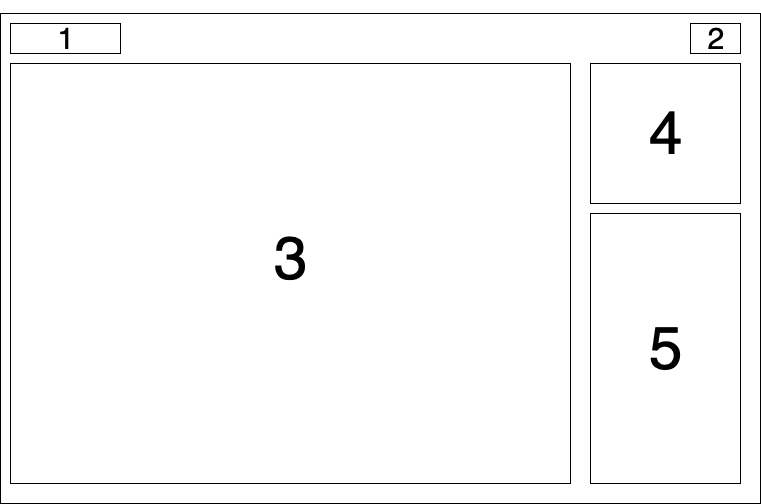
\includegraphics[width=0.75\textwidth]{Rysunki/Rozdzial06/Glowne_okno_koncepcja.png}
    \caption{Okno główne aplikacji}
    \label{Okno glowne}
\end{figure}

\newpage
%----------------------------------------------------------------------------------------------------------------
\section{Zrzuty ekranu}

\begin{figure}[h!]
    \centering
    \includegraphics[width=1\textwidth]{Rysunki/Rozdzial06/Okno_laczenia.png}
    \caption{Okno do łączenia się z robotem}
    \label{Okno laczenie}
\end{figure}

\begin{figure}[h!]
    \centering
    \includegraphics[width=1\textwidth]{Rysunki/Rozdzial06/Panel_sterowania.png}
    \caption{Okno z panelem operatorskim}
    \label{Okno panel}
\end{figure}

\begin{figure}[h!]
    \centering
    \includegraphics[width=1\textwidth]{Rysunki/Rozdzial06/Fuzja.png}
    \caption{Okno z wykresami dotyczącymi fuzji sygnałów}
    \label{Okno fuzja}
\end{figure}

\begin{figure}[h!]
    \centering
    \includegraphics[width=1\textwidth]{Rysunki/Rozdzial06/Zyro.png}
    \caption{Okno z wykresami dotyczącymi żyroskopu}
    \label{Okno zyro}
\end{figure}

%----------------------------------------------------------------------------------------------------------------
\chapter{Testy eksperymentalne}

%\bibliographystyle{plalpha}
\bibliographystyle{plabbrv}

%UWAGA: bibliotekę referencji należy przygotować samemu. Dobrym do tego narzędziem jest JabRef.
%       Nazwę przygotowanej biblioteki wpisuje się poniżej bez rozszerzenia 
%       (w tym przypadku jest to "dokumentacja.bib")
\bibliography{dokumentacja}
\appendix
%\chapter{Tytuł dodatku}
Zasady przyznawania stopnia naukowego doktora i doktora habilitowanego w Polsce określa ustawa z dnia 14 marca 2003 r. o stopniach naukowych i~tytule naukowym oraz o stopniach i~tytule w zakresie sztuki (Dz.U. nr 65 z 2003 r., poz. 595 (Dz. U. z 2003 r. Nr 65, poz. 595). Poprzednie polskie uregulowania nie wymagały bezwzględnie posiadania przez kandydata tytułu zawodowego magistra lub równorzędnego (choć zasada ta zazwyczaj była przestrzegana) i zdarzały się nadzwyczajne przypadki nadawania stopnia naukowego doktora osobom bez studiów wyższych, np. słynnemu matematykowi lwowskiemu – późniejszemu profesorowi Stefanowi Banachowi. 

W innych krajach również zazwyczaj do przyznania stopnia naukowego doktora potrzebny jest dyplom ukończenia uczelni wyższej, ale nie wszędzie.


%\chapter{Opis załączonej płyty CD/DVD}
Tutaj jest miejsce na zamieszczenie opisu zawartości załączonej płyty.
Należy wymienić, co zawiera. 

\chapterstyle{noNumbered}
\phantomsection % sets an anchor
%\addcontentsline{toc}{chapter}{Indeks rzeczowy}
\printindex

\end{document}
